\documentclass{beamer}
\usetheme{default}


\usepackage{adjustbox}
\usepackage{listings}

\usepackage{tabularray}
\usepackage{float}
\usepackage{graphicx}
\usepackage{codehigh}
\usepackage[normalem]{ulem}
\usepackage{anyfontsize}
\UseTblrLibrary{booktabs}
\UseTblrLibrary{siunitx}
\newcommand{\tinytableTabularrayUnderline}[1]{\underline{#1}}
\newcommand{\tinytableTabularrayStrikeout}[1]{\sout{#1}}
\NewTableCommand{\tinytableDefineColor}[3]{\definecolor{#1}{#2}{#3}}

\title{Análise exploratória}
\author{Victor Batista}
\begin{document}

\begin{frame}[plain]
    \maketitle
\end{frame}

\begin{frame}{Socioeconômicas}
	\begin{table}
		\tiny
		\centering
		\begin{tblr}[         %% tabularray outer open
			]                     %% tabularray outer close
			{                     %% tabularray inner open
				colspec={Q[]Q[]Q[]Q[]Q[]Q[]Q[]Q[]Q[]},
				column{1}={halign=l,},
				column{2}={halign=l,},
				column{3}={halign=l,},
				column{4}={halign=l,},
				column{5}={halign=l,},
				column{6}={halign=l,},
				column{7}={halign=l,},
				column{8}={halign=l,},
				column{9}={halign=l,},
			}                     %% tabularray inner close
			\toprule
			& Unique & Missing Pct. & Mean & SD & Min & Median & Max & Histogram \\ \midrule %% TinyTableHeader
			Taxa\_de\_analfabetismo          & 220  & 0 & 9.9     & 5.7     & 0.9    & 9.1     & 40.2     &  \\
			Taxa\_de\_desemprego\_16a\_e+      & 643  & 0 & 4.1     & 2.7     & 0.1    & 3.8     & 27.8     &  \\
			Gini                           & 898  & 0 & 0.5     & 0.1     & 0.3    & 0.5     & 0.8      &  \\
			PIB\_per\_capita                 & 1130 & 0 & 16374.5 & 12533.7 & 3129.3 & 13963.5 & 220358.3 &  \\
			população\_com\_renda\_<\_1/4\_SM & 934  & 0 & 13.9    & 13.0    & 0.1    & 9.9     & 77.9     &  \\
			Taxa\_de\_trabalho\_infantil      & 932  & 0 & 17.2    & 10.8    & 0.3    & 14.5    & 72.1     &  \\
			Porcentagem\_Homens\_Jovens      & 498  & 0 & 12.5    & 1.5     & 7.9    & 12.4    & 26.7     &  \\
			\bottomrule
		\end{tblr}
	\end{table}	
\end{frame}

\begin{frame}{Homicídios}
	\begin{table}
		\tiny
		\centering
		\begin{tblr}[         %% tabularray outer open
			]                     %% tabularray outer close
			{                     %% tabularray inner open
				colspec={Q[]Q[]Q[]Q[]Q[]Q[]Q[]Q[]Q[]},
				column{1}={halign=l,},
				column{2}={halign=l,},
				column{3}={halign=l,},
				column{4}={halign=l,},
				column{5}={halign=l,},
				column{6}={halign=l,},
				column{7}={halign=l,},
				column{8}={halign=l,},
				column{9}={halign=l,},
			}                     %% tabularray inner close
			\toprule
			& Unique & Missing Pct. & Mean & SD & Min & Median & Max & Histogram \\ \midrule %% TinyTableHeader
			valor-2010 & 658 & 0 & 15.5 & 18.7 & 0.0 & 10.2 & 147.4 &  \\
			valor-2011 & 620 & 0 & 14.1 & 17.3 & 0.0 & 9.1  & 111.1 &  \\
			valor-2012 & 648 & 0 & 16.1 & 19.3 & 0.0 & 10.9 & 132.0 &  \\
			valor-2013 & 662 & 0 & 15.9 & 19.8 & 0.0 & 11.7 & 183.7 &  \\
			valor-2014 & 680 & 0 & 16.4 & 19.0 & 0.0 & 11.8 & 153.9 &  \\
			valor-2015 & 671 & 0 & 16.5 & 19.1 & 0.0 & 11.8 & 137.1 &  \\
			valor-2016 & 690 & 0 & 18.2 & 20.7 & 0.0 & 13.2 & 155.1 &  \\
			valor-2017 & 706 & 0 & 19.6 & 22.2 & 0.0 & 14.6 & 222.0 &  \\
			valor-2018 & 678 & 0 & 16.9 & 20.3 & 0.0 & 12.4 & 211.0 &  \\
			valor-2019 & 657 & 0 & 15.5 & 19.2 & 0.0 & 10.9 & 176.7 &  \\
			\bottomrule
		\end{tblr}
	\end{table}
	
\end{frame}

\begin{frame}{Outros crimes}
	\begin{table}
		\tiny
		\centering
		\begin{tblr}[         %% tabularray outer open
			]                     %% tabularray outer close
			{                     %% tabularray inner open
				colspec={Q[]Q[]Q[]Q[]Q[]Q[]Q[]Q[]Q[]},
				column{1}={halign=l,},
				column{2}={halign=l,},
				column{3}={halign=l,},
				column{4}={halign=l,},
				column{5}={halign=l,},
				column{6}={halign=l,},
				column{7}={halign=l,},
				column{8}={halign=l,},
				column{9}={halign=l,},
			}                     %% tabularray inner close
			\toprule
			& Unique & Missing Pct. & Mean & SD & Min & Median & Max & Histogram \\ \midrule %% TinyTableHeader
			feminicidio\_pc   & 156 & 0 & 1.4  & 6.5    & 0.0 & 0.0  & 101.7   &  \\
			hom\_doloso\_pc    & 621 & 0 & 31.7 & 263.5  & 0.0 & 6.0  & 8203.4  &  \\
			lesao\_pc         & 74  & 0 & 0.9  & 6.9    & 0.0 & 0.0  & 169.5   &  \\
			mandado\_pc       & 625 & 0 & 98.5 & 173.8  & 0.0 & 21.1 & 1285.4  &  \\
			transito\_pc      & 588 & 0 & 20.1 & 86.6   & 0.0 & 3.2  & 2474.6  &  \\
			esclarecer\_pc    & 531 & 0 & 58.4 & 1096.0 & 0.0 & 0.0  & 36508.5 &  \\
			latrocinio\_pc    & 138 & 0 & 1.7  & 11.4   & 0.0 & 0.0  & 305.1   &  \\
			tentativa\_hom\_pc & 570 & 0 & 26.8 & 164.6  & 0.0 & 2.3  & 4678.0  &  \\
			\bottomrule
		\end{tblr}
	\end{table}
	
\end{frame}

\begin{frame}{Categóricas}
	\begin{table}
		\centering
		\begin{tblr}[         %% tabularray outer open
			]                     %% tabularray outer close
			{                     %% tabularray inner open
				colspec={Q[]Q[]Q[]Q[]},
				column{1}={halign=l,},
				column{2}={halign=l,},
				column{3}={halign=r,},
				column{4}={halign=r,},
			}                     %% tabularray inner close
			\toprule
			&    & N & \%  \\ \midrule %% TinyTableHeader
			name\_state  & Acre               & 22  & 1.9  \\
			& Amapá              & 15  & 1.3  \\
			& Amazônas           & 32  & 2.8  \\
			& Mato Grosso        & 57  & 5.0  \\
			& Mato Grosso do Sul & 66  & 5.8  \\
			& Pará               & 7   & 0.6  \\
			& Paraná             & 297 & 26.2 \\
			& Rio Grande do Sul  & 413 & 36.5 \\
			& Rondônia           & 52  & 4.6  \\
			& Roraima            & 15  & 1.3  \\
			& Santa Catarina     & 144 & 12.7 \\
			& São Paulo          & 12  & 1.1  \\
			\bottomrule
		\end{tblr}
	\end{table}
\end{frame}

\begin{frame}{Categóricas}
	\begin{table}
		\centering
		\begin{tblr}[         %% tabularray outer open
			]                     %% tabularray outer close
			{                     %% tabularray inner open
				colspec={Q[]Q[]Q[]Q[]},
				column{1}={halign=l,},
				column{2}={halign=l,},
				column{3}={halign=r,},
				column{4}={halign=r,},
			}                     %% tabularray inner close
			\toprule
			&    & N &  \% \\ \midrule %% TinyTableHeader
			name\_region & Centro Oeste       & 123 & 10.9 \\
			& Norte              & 143 & 12.6 \\
			& Sudeste            & 12  & 1.1  \\
			& Sul                & 854 & 75.4 \\
			groups      & control            & 544 & 48.1 \\
			& treatment          & 588 & 51.9 \\
			arcos       & Arco Central       & 175 & 15.5 \\
			& Arco Norte         & 91  & 8.0  \\
			& Arco Sudeste       & 12  & 1.1  \\
			& Arco Sul           & 854 & 75.4 \\
			\bottomrule
		\end{tblr}
	\end{table}
\end{frame}

\begin{frame}
\begin{figure}
	\centering
	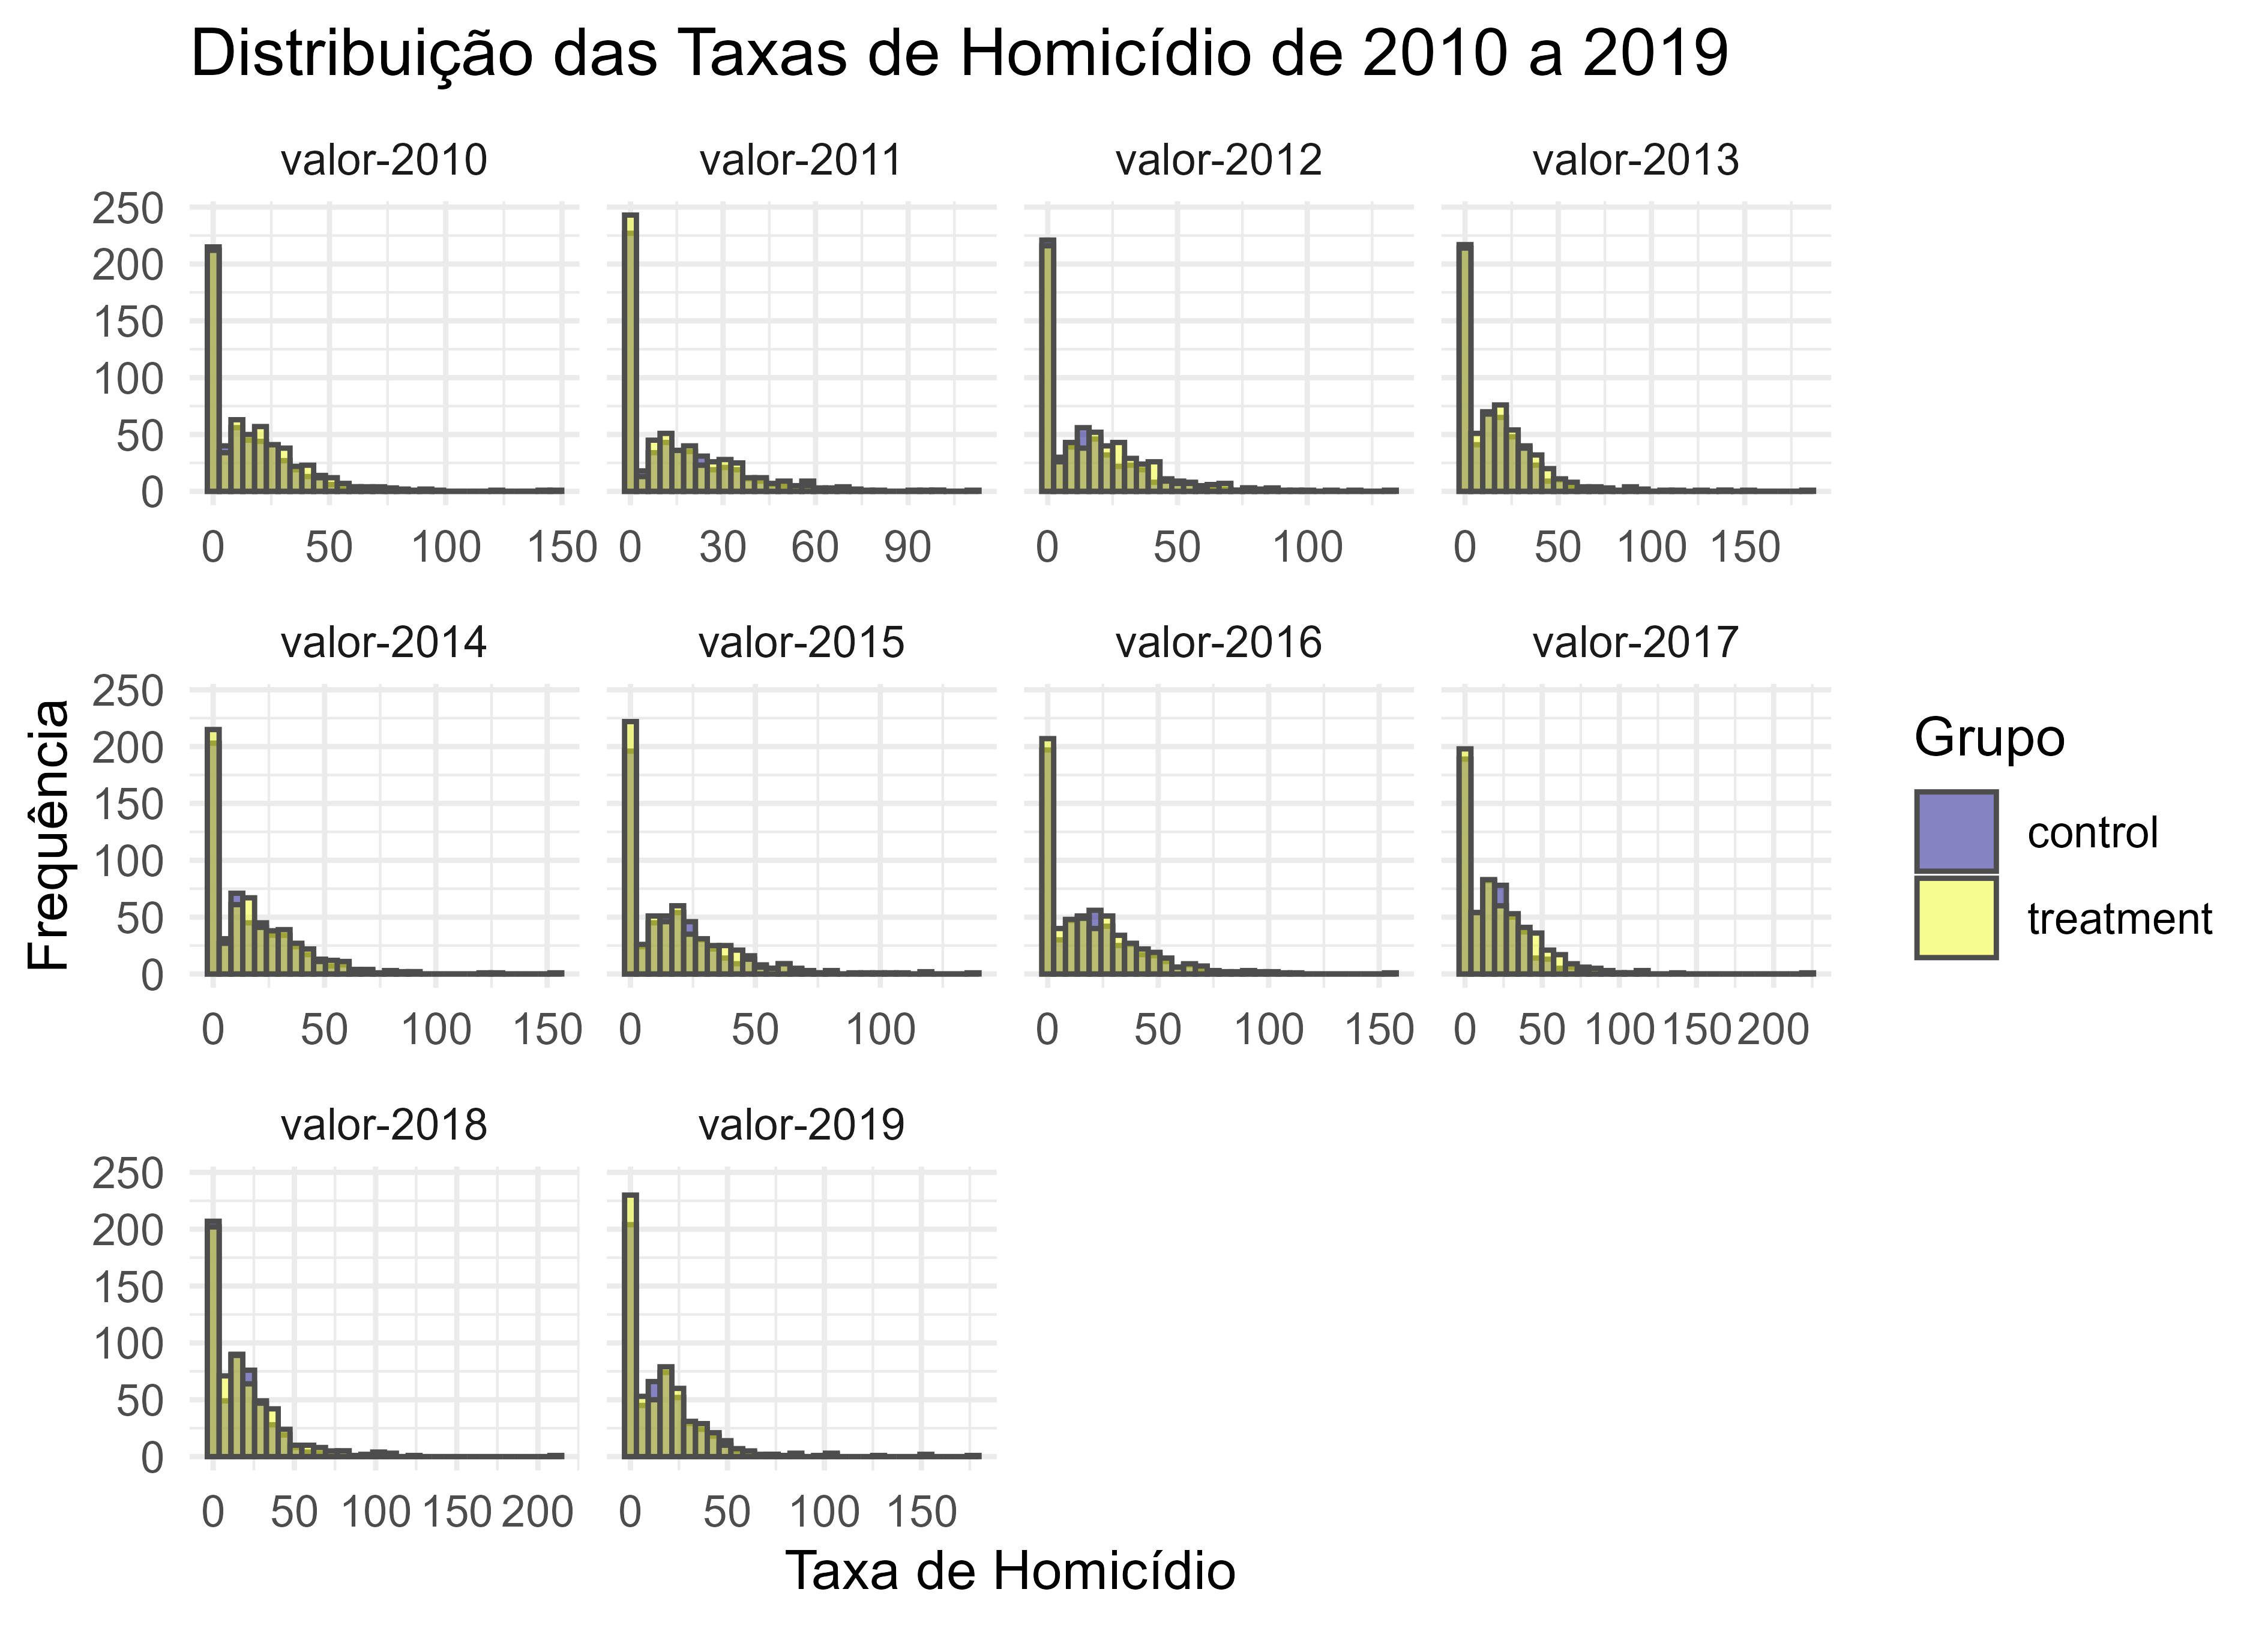
\includegraphics[width=1\linewidth]{figures/histog_hom}
	\label{fig:histoghom}
\end{figure}

\end{frame}

\begin{frame}
	\begin{figure}
		\centering
		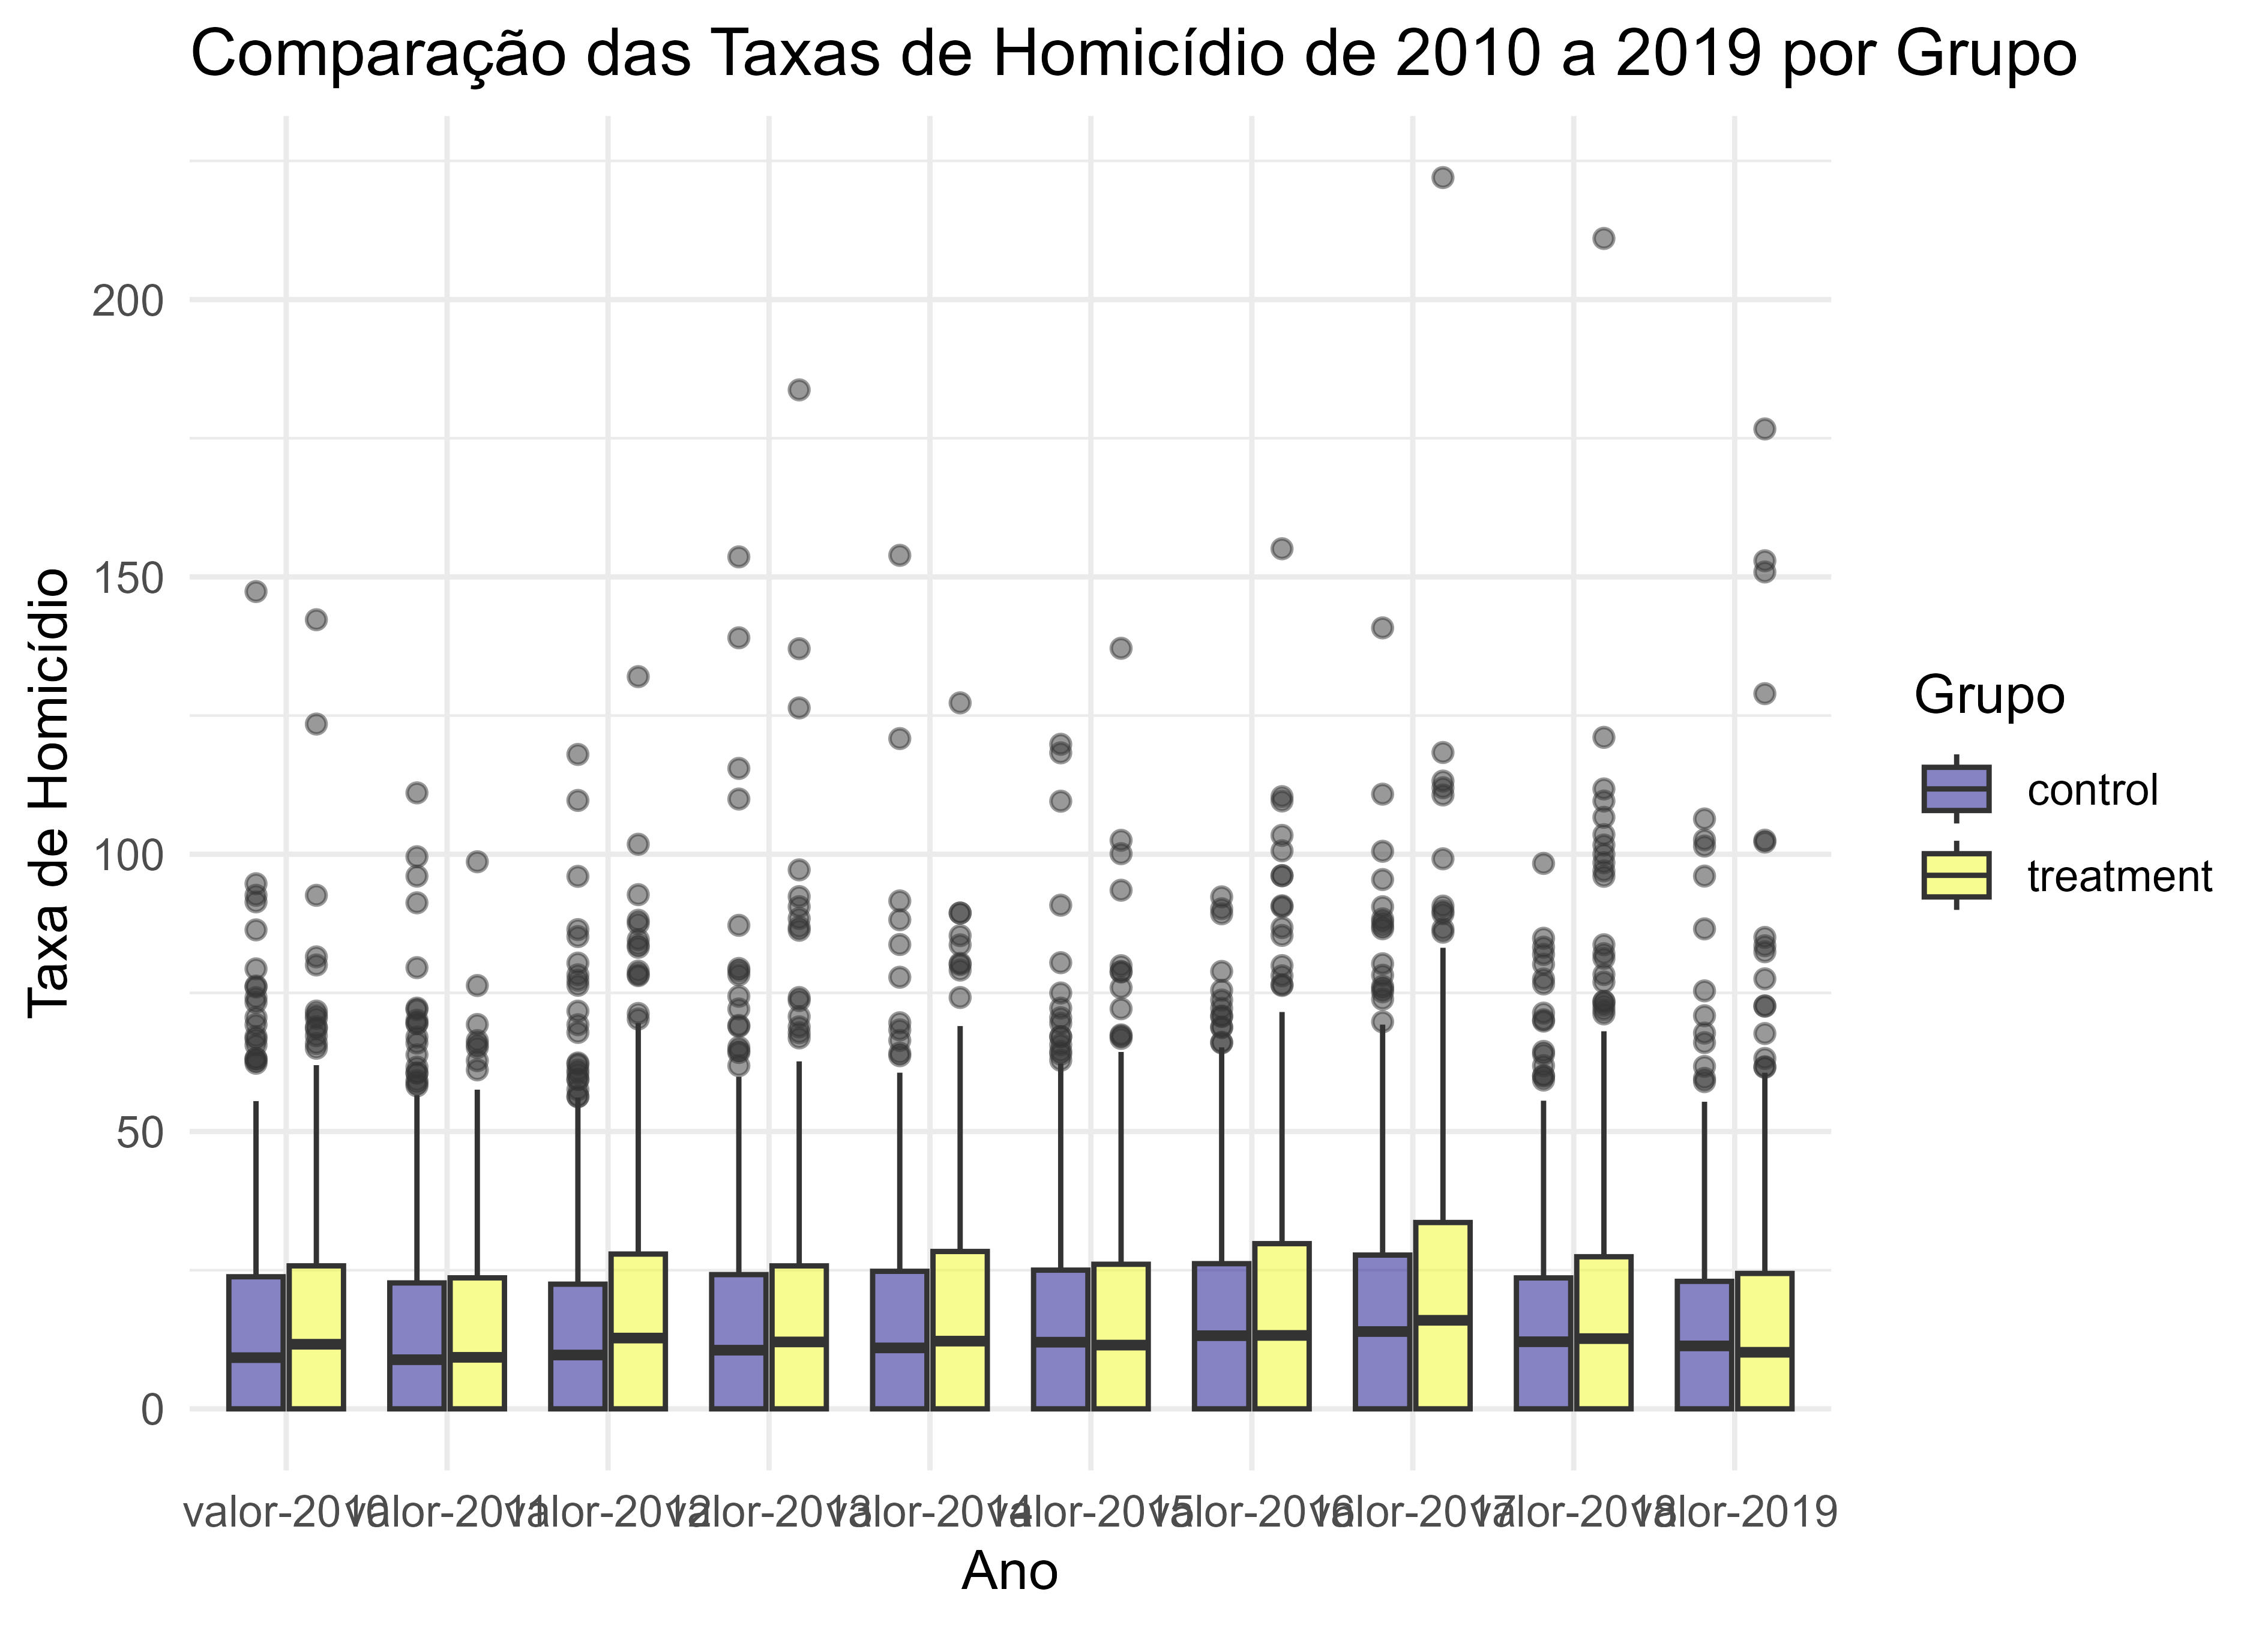
\includegraphics[width=1\linewidth]{figures/boxplot_hom}
		\label{fig:histoghom}
	\end{figure}
	
\end{frame}

\begin{frame}
	\begin{figure}
		\centering
		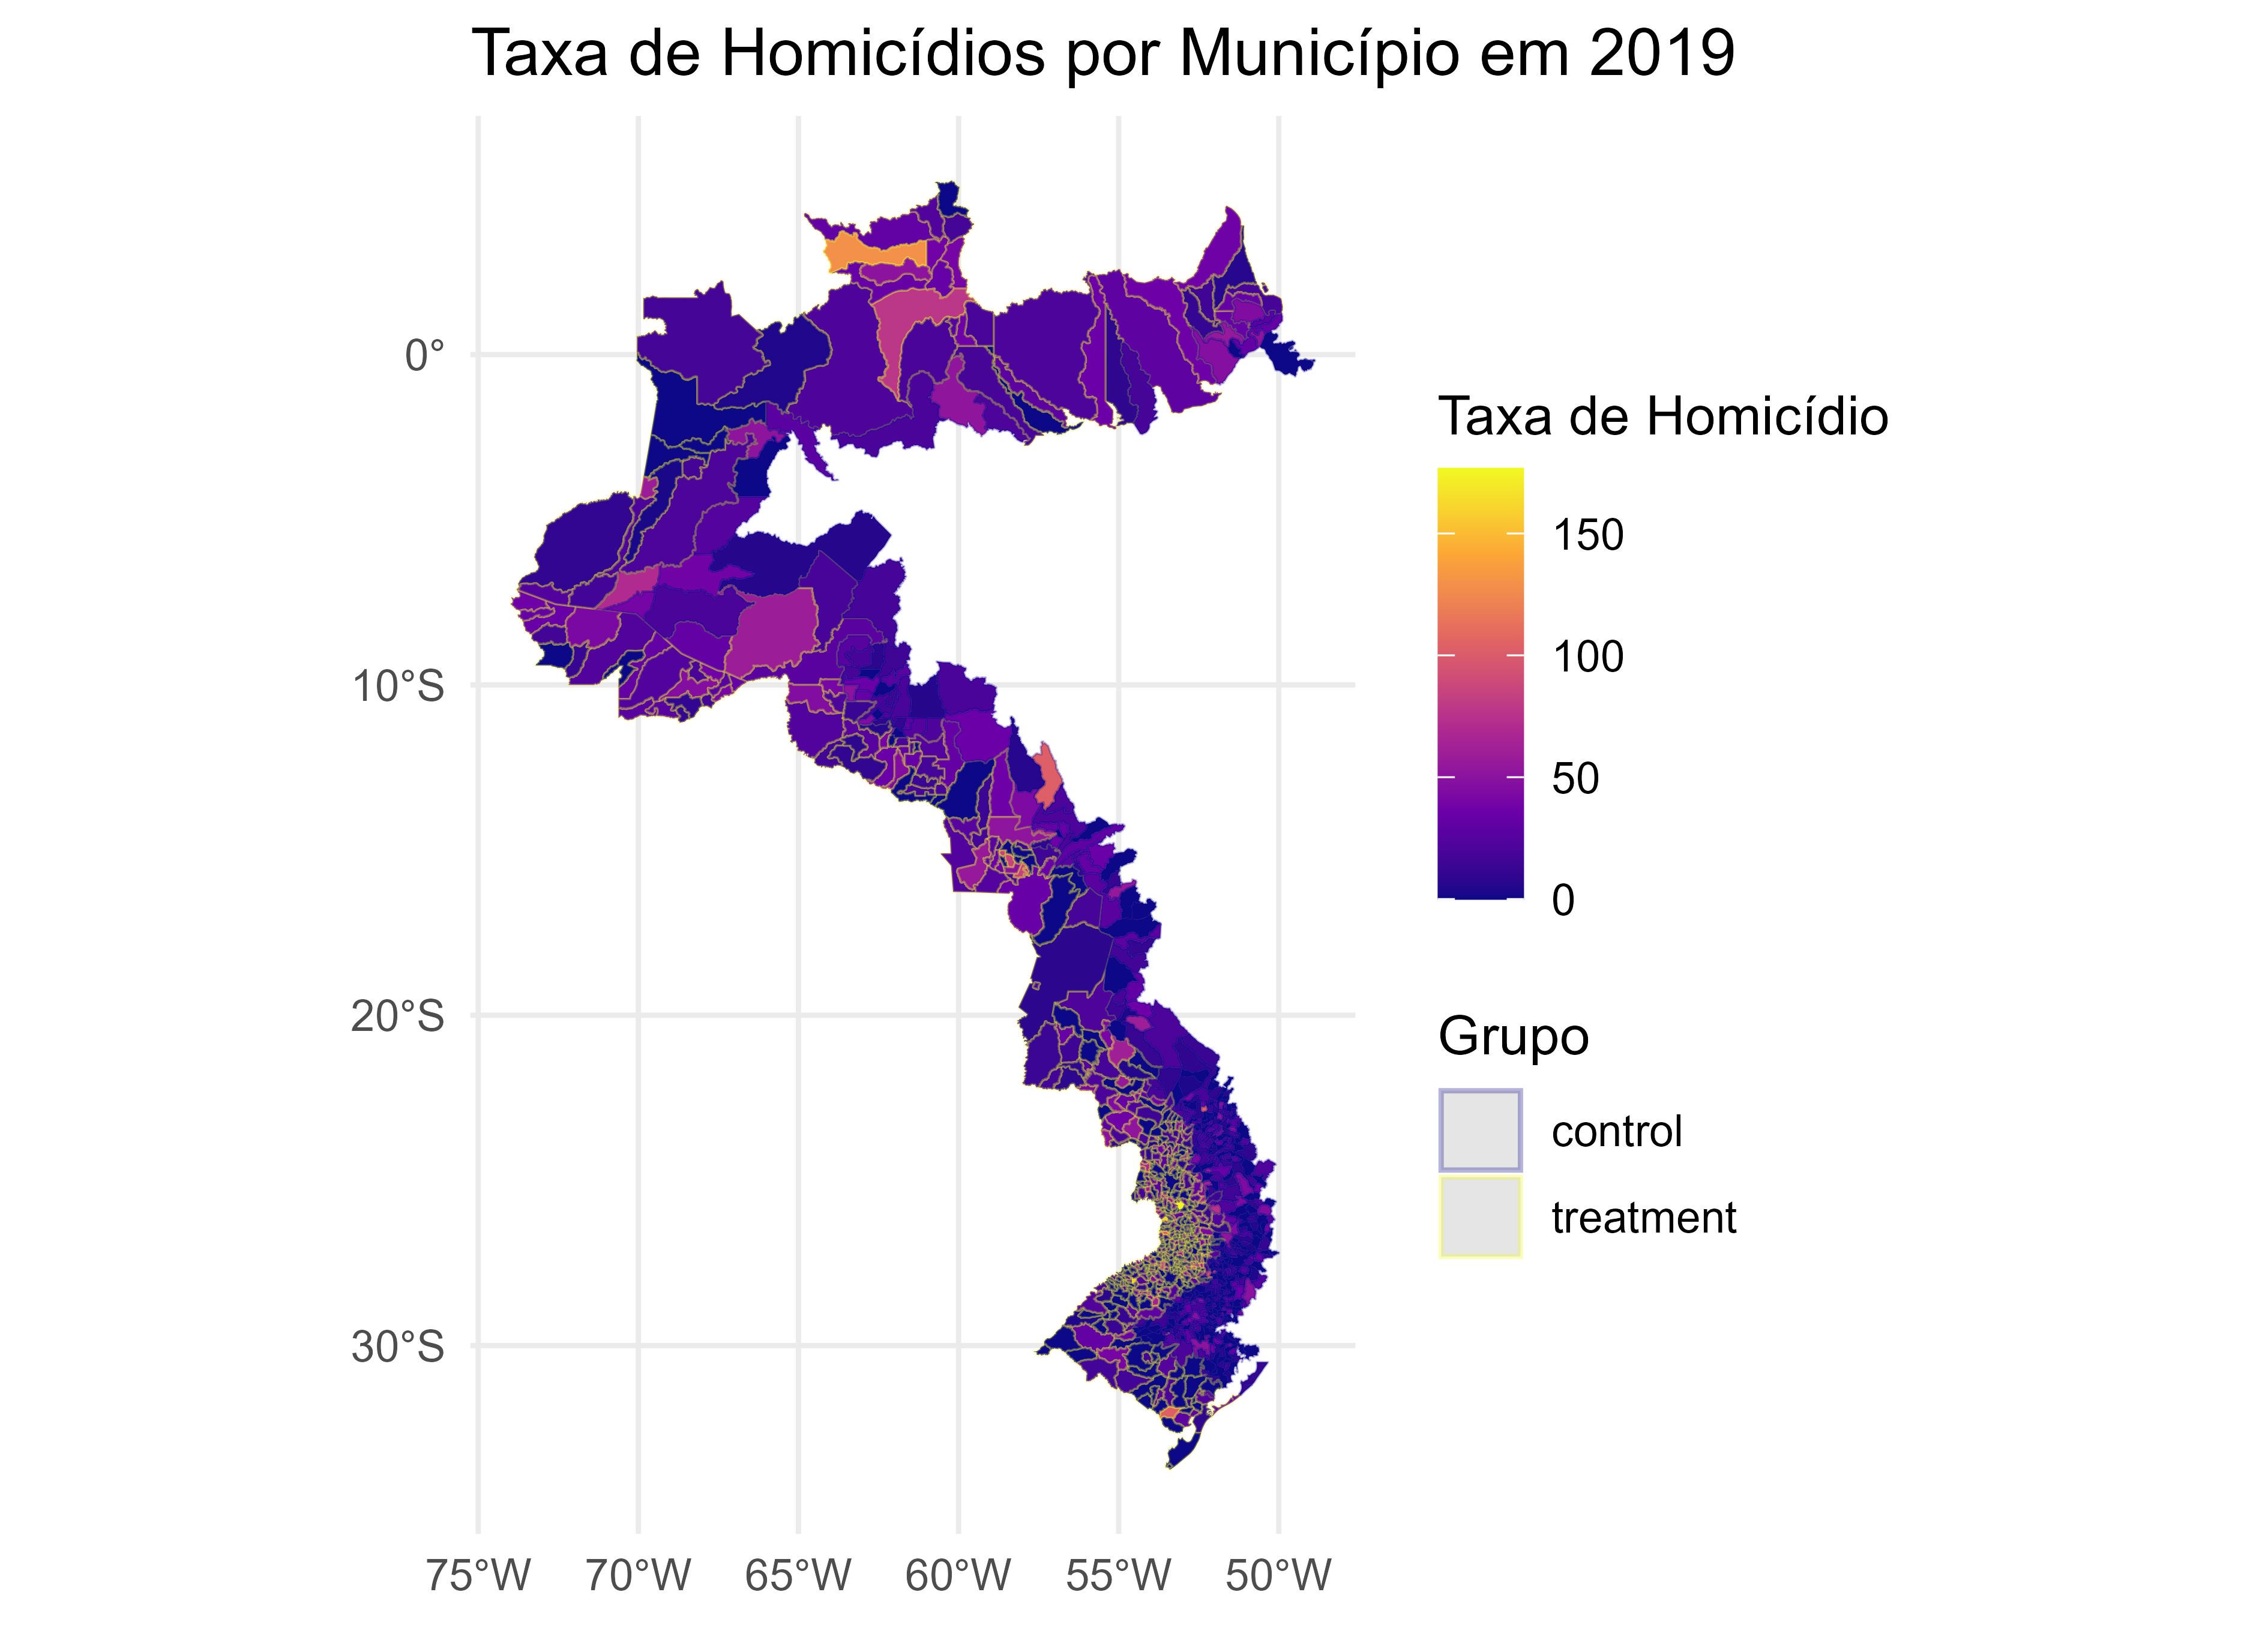
\includegraphics[width=1\linewidth]{figures/mapa_hom_2019}
		\label{fig:histoghom}
	\end{figure}
	
\end{frame}

\begin{frame}
	\begin{figure}
		\centering
		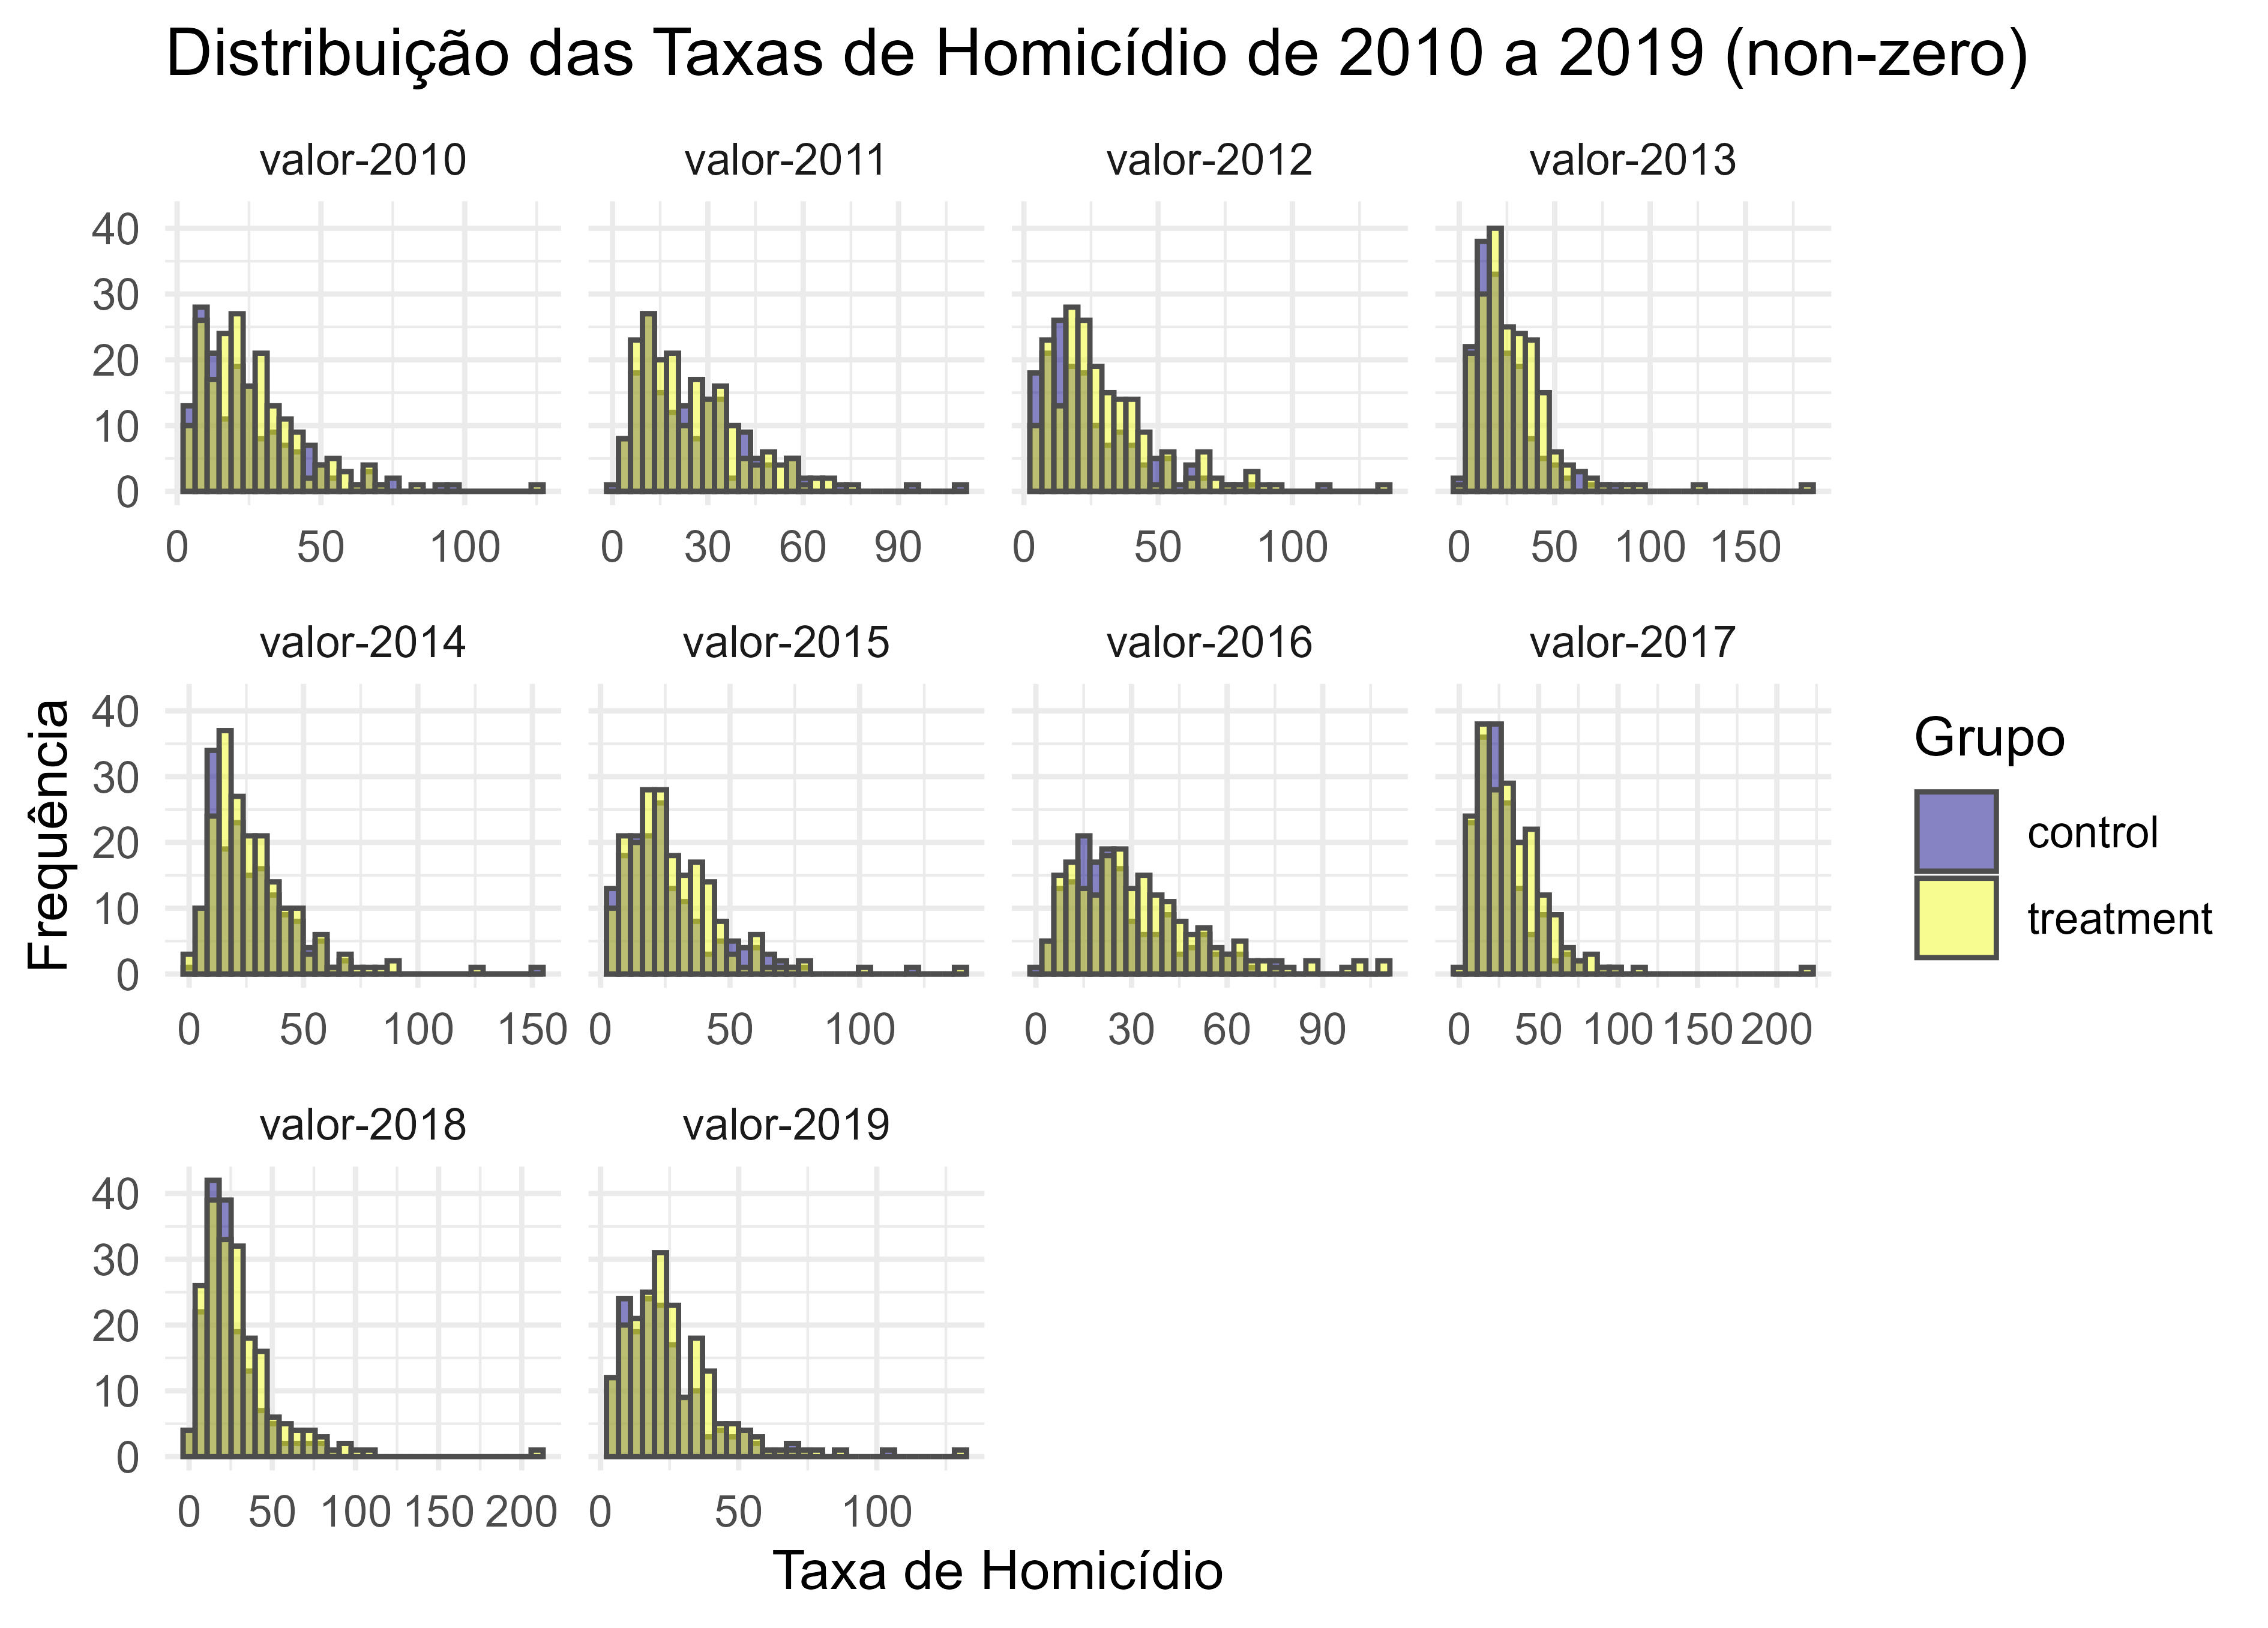
\includegraphics[width=1\linewidth]{figures/histog_hom_nonzero}
		\label{fig:histoghom}
	\end{figure}
	
\end{frame}

\begin{frame}
	\begin{figure}
		\centering
		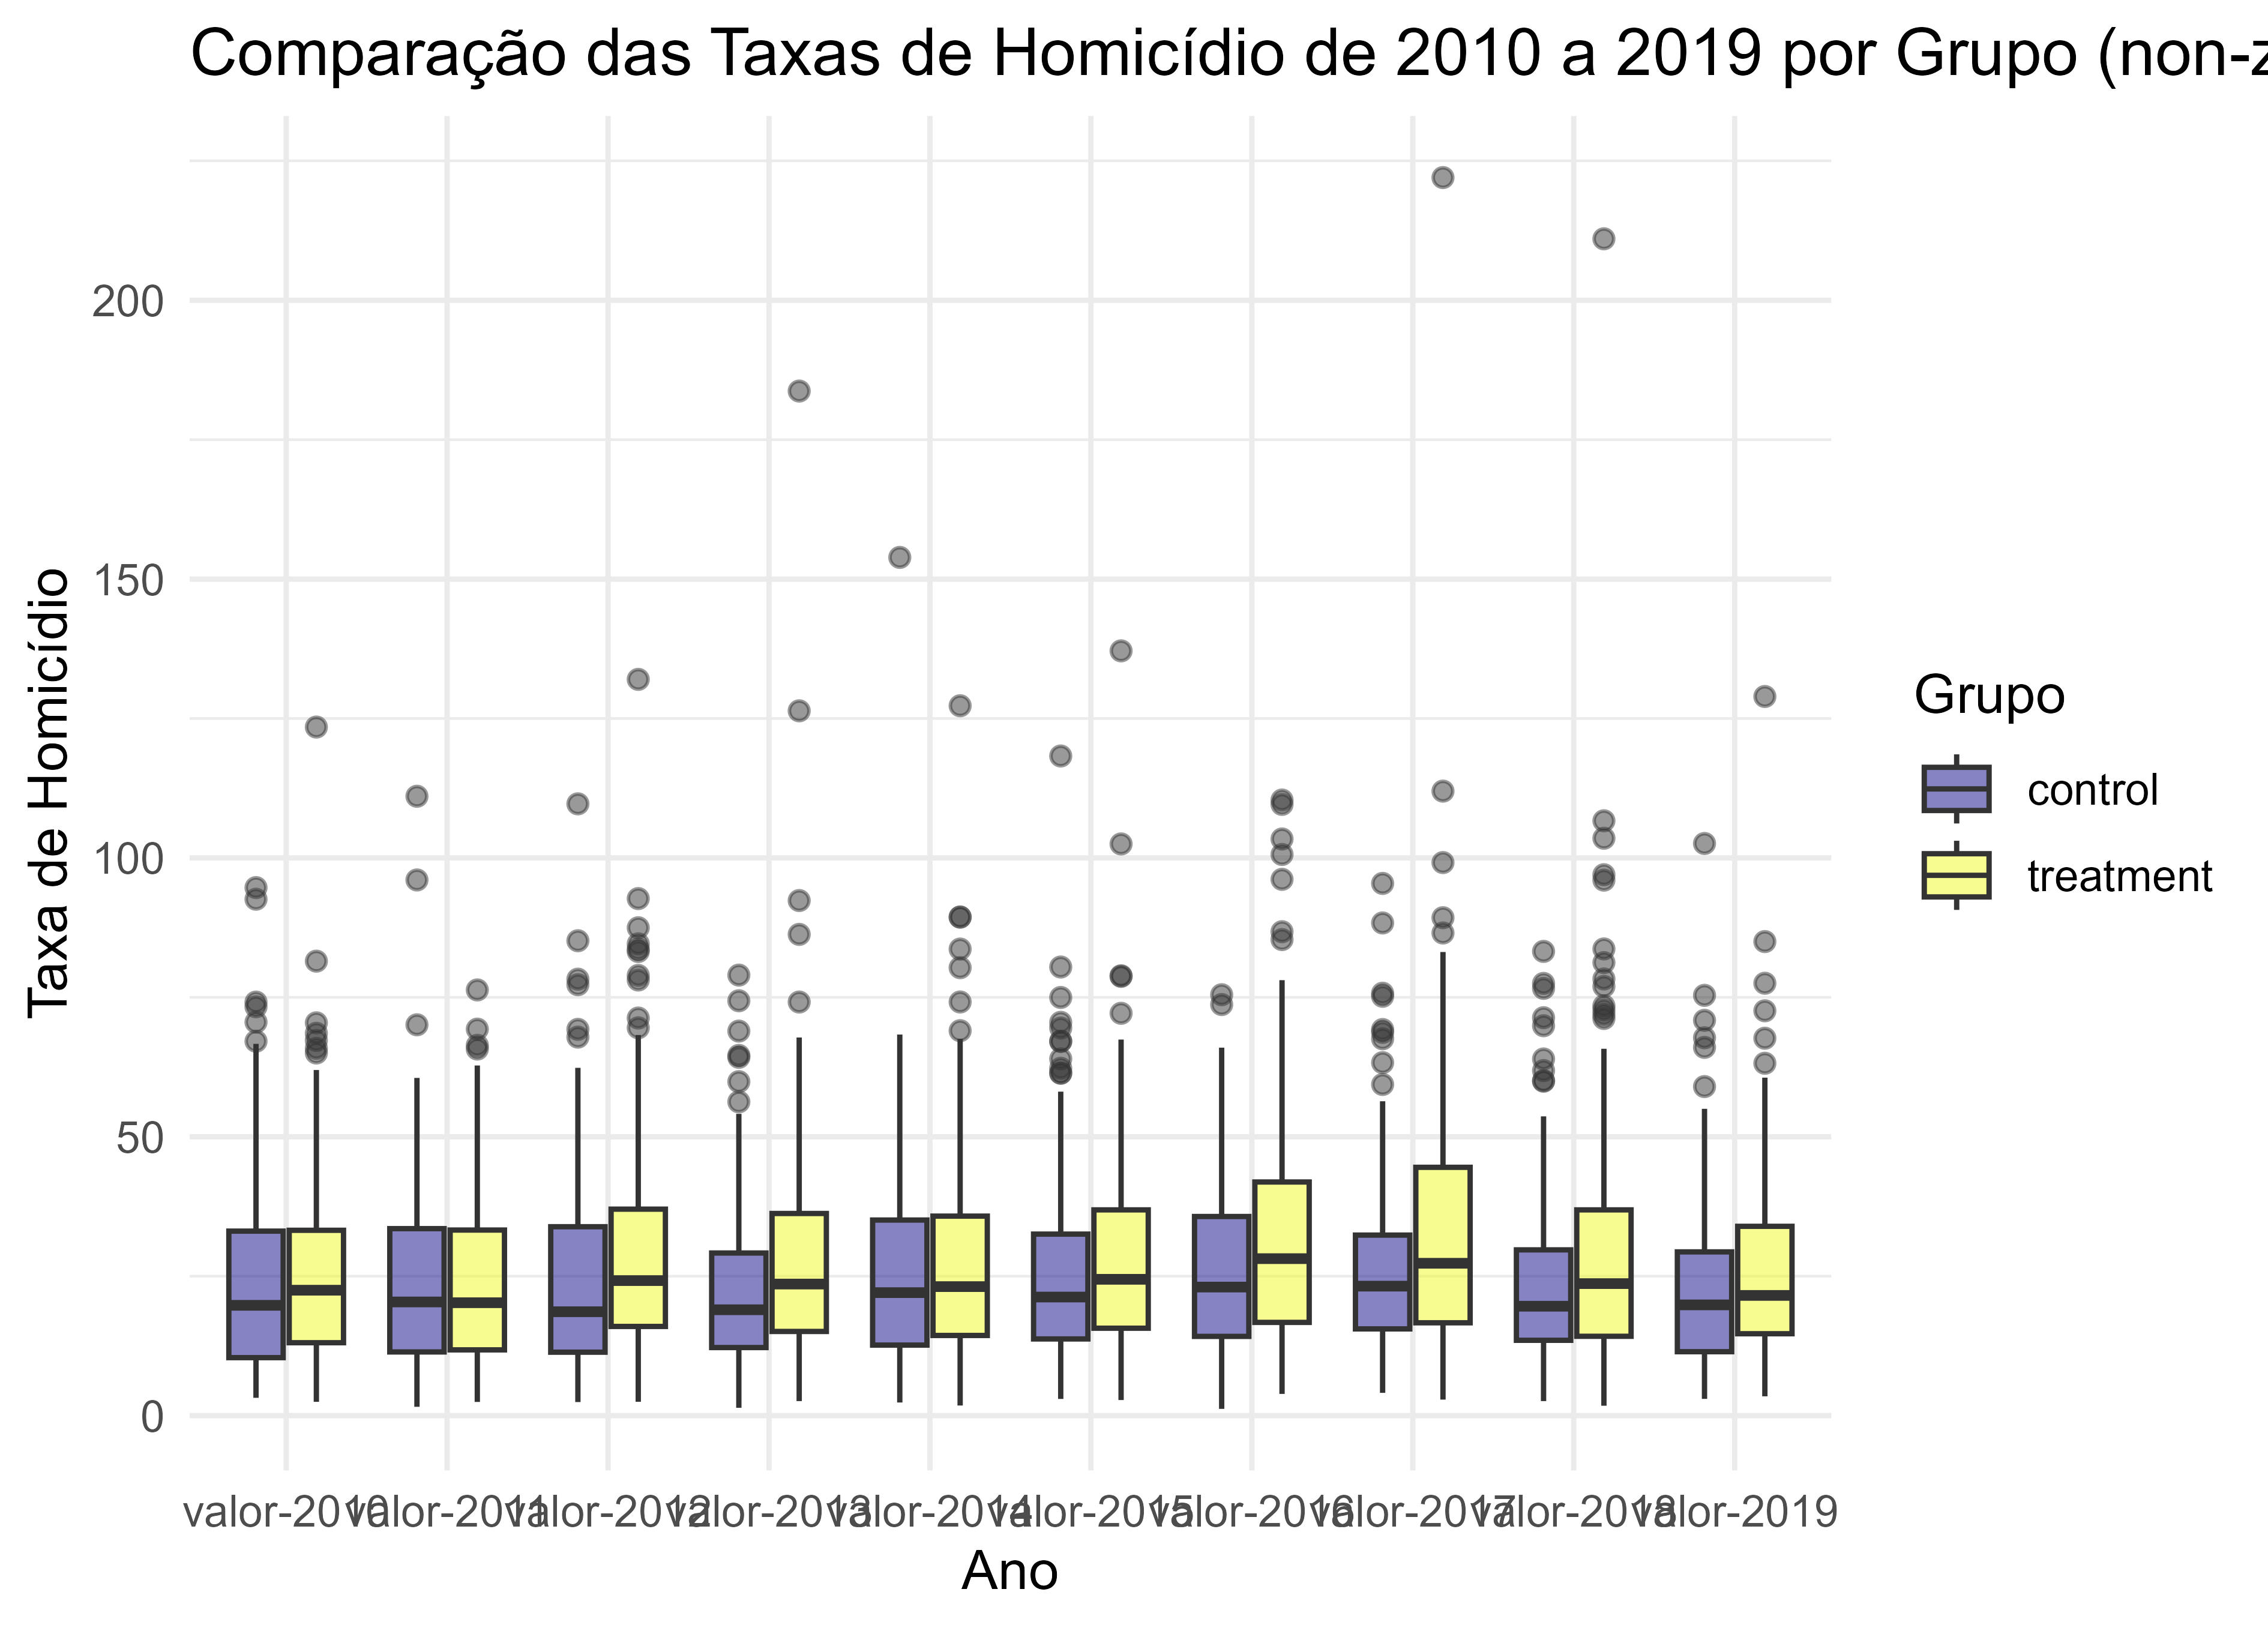
\includegraphics[width=1\linewidth]{figures/boxplot_hom_nonzero}
		\label{fig:histoghom}
	\end{figure}
	
\end{frame}

\begin{frame}
	\begin{figure}
		\centering
		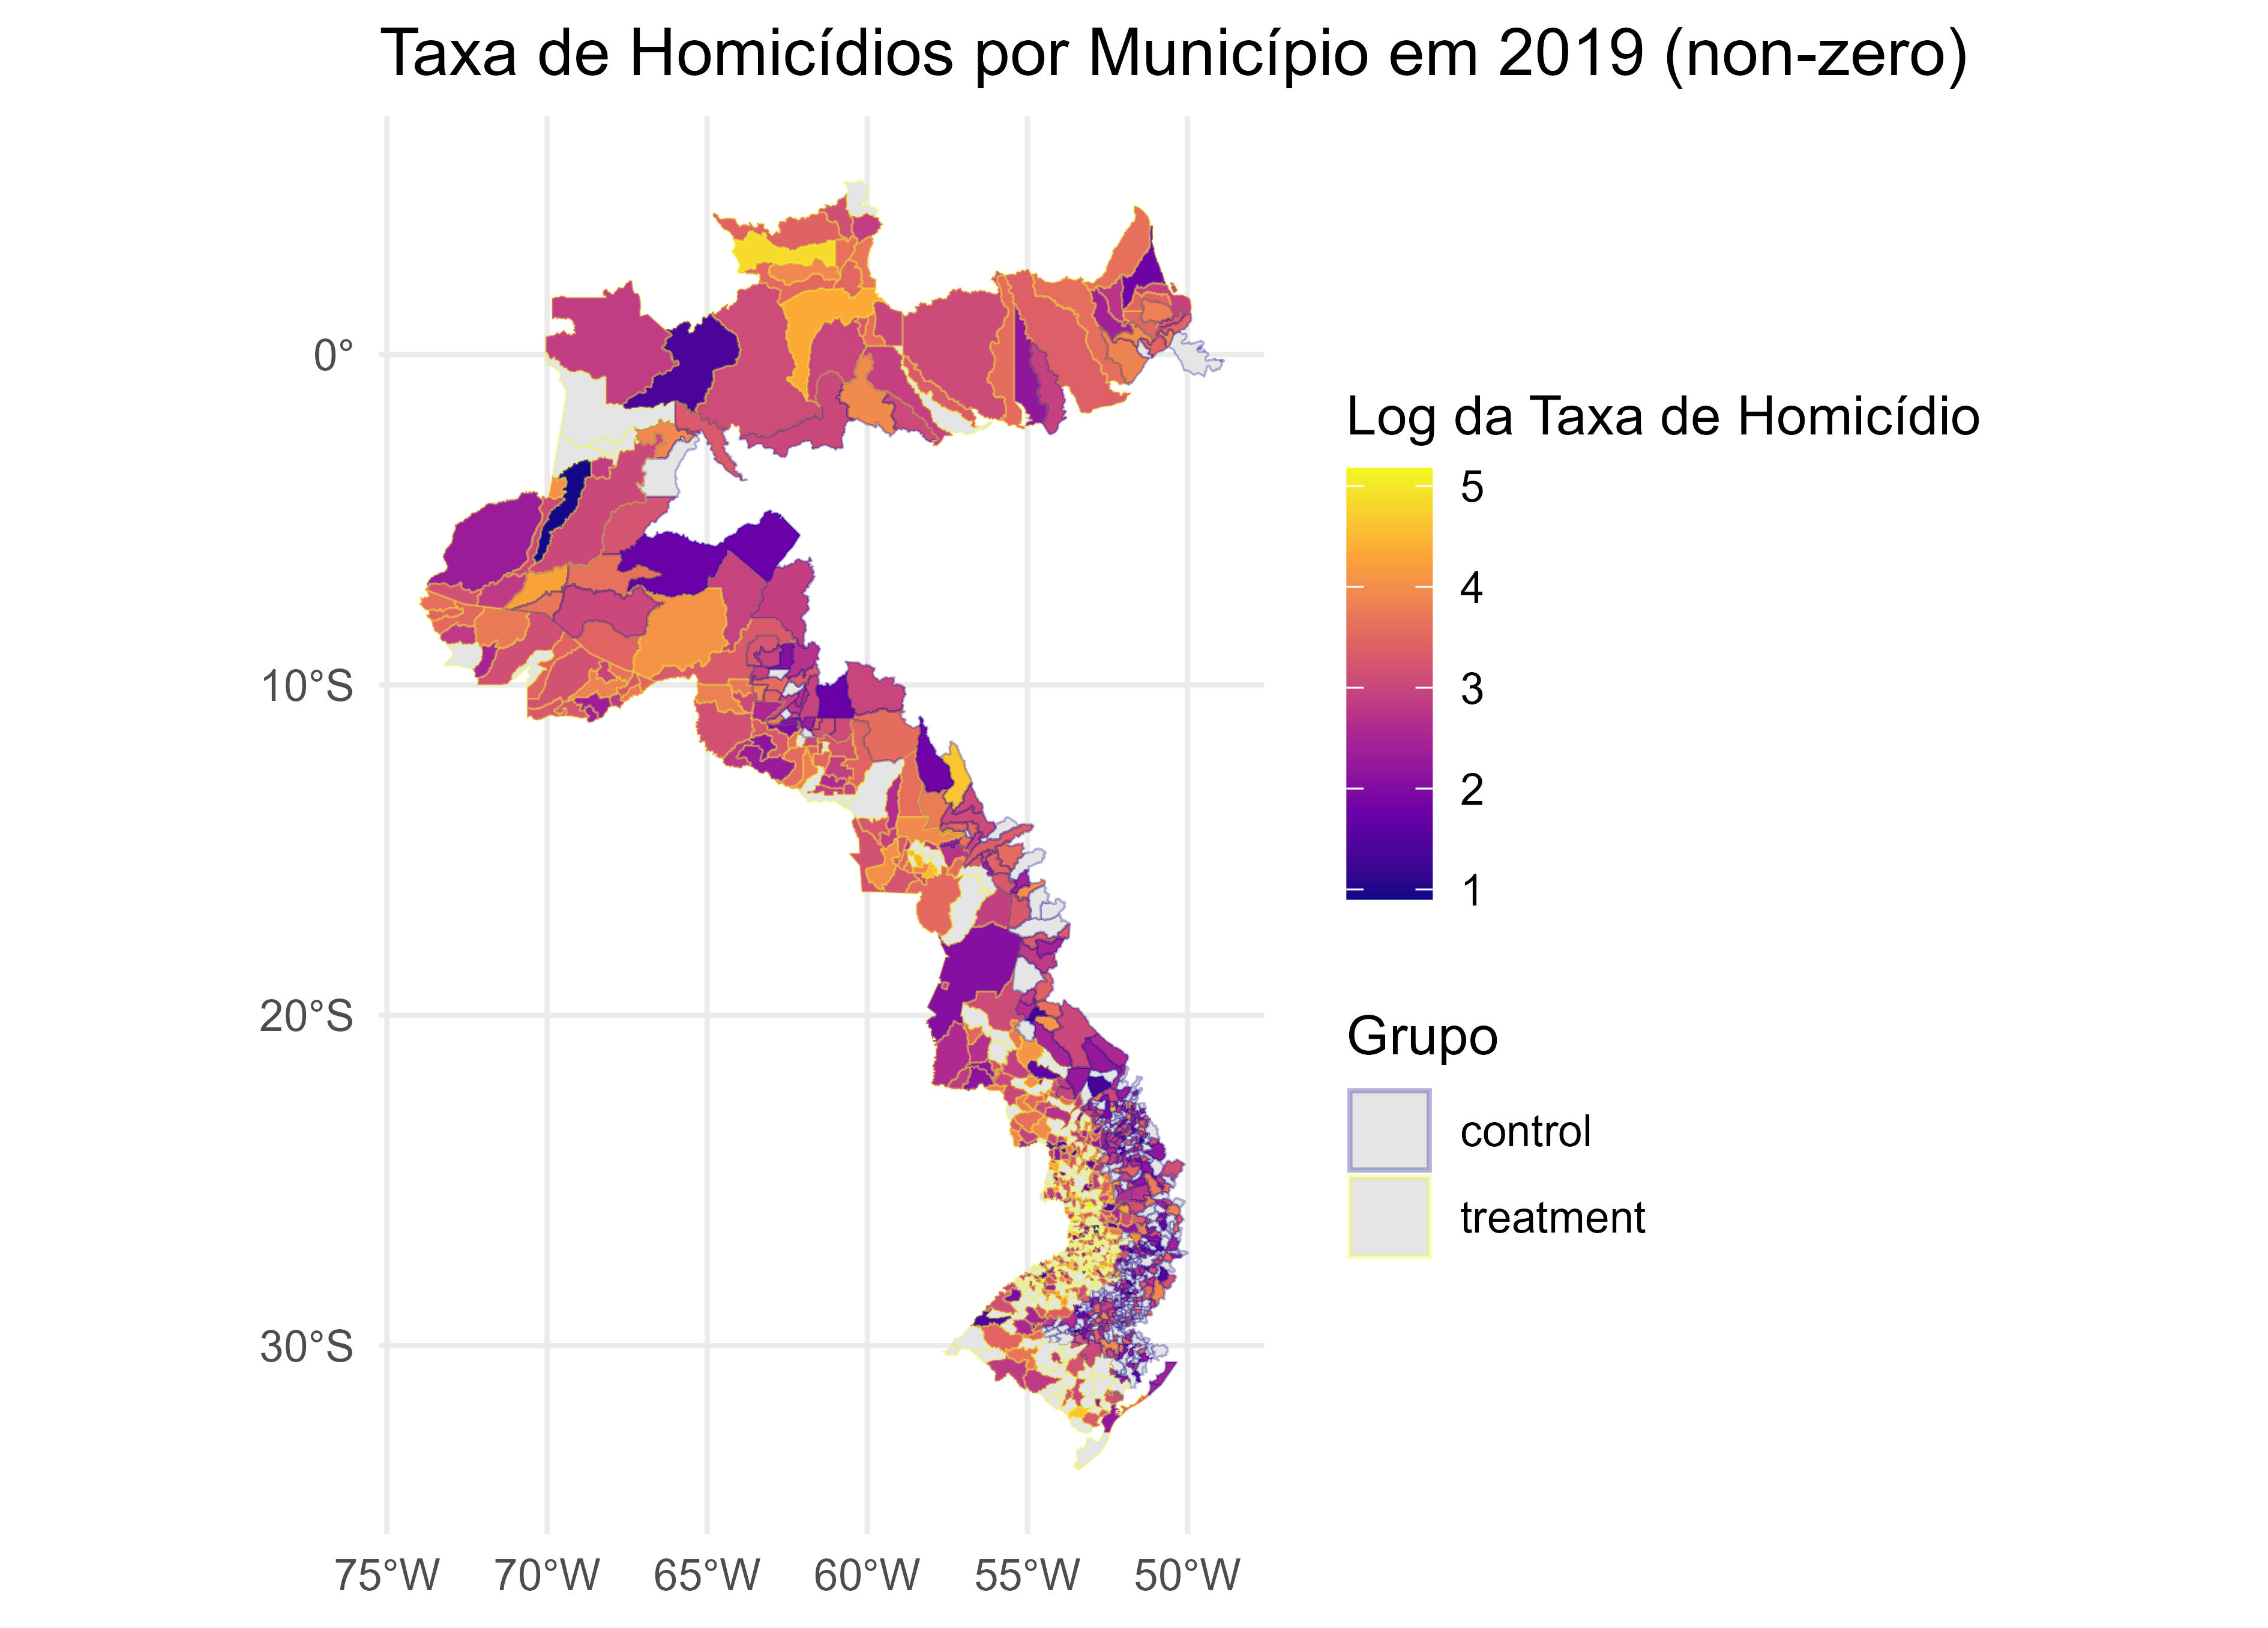
\includegraphics[width=1\linewidth]{figures/mapa_hom_2019_nonzero}
		\label{fig:histoghom}
	\end{figure}
\end{frame}

\begin{frame}
	\begin{figure}
		\centering
		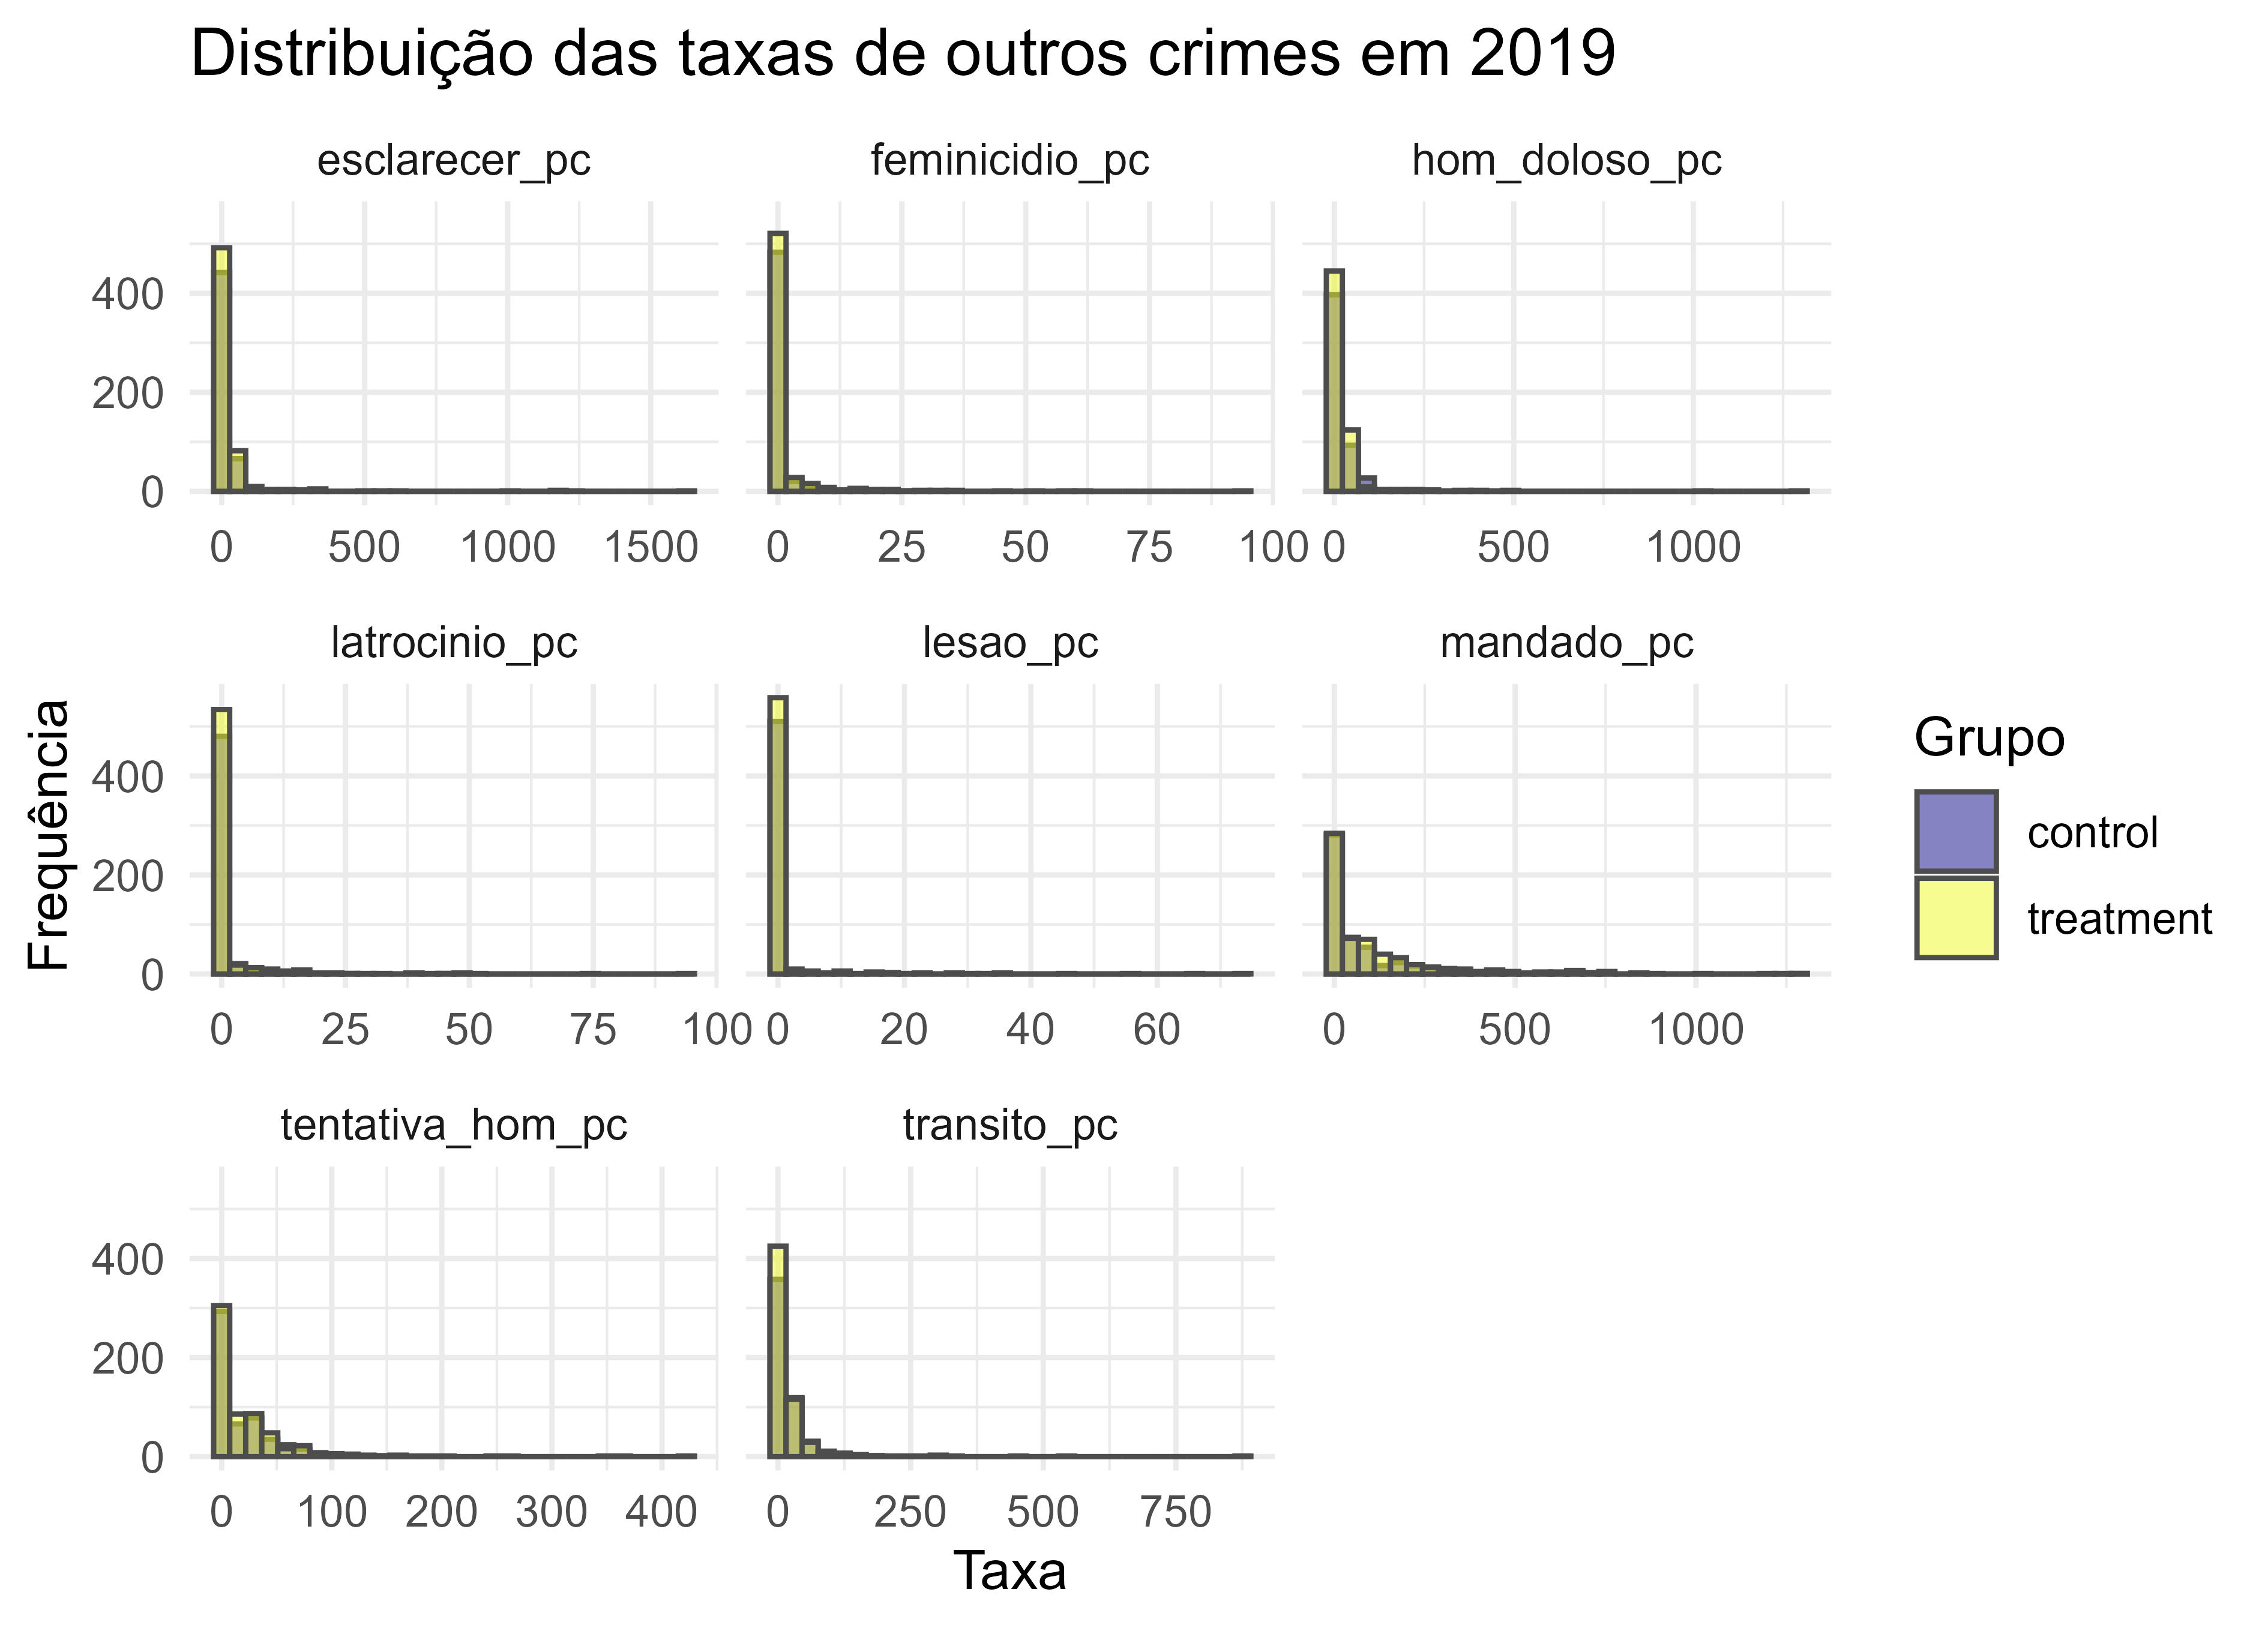
\includegraphics[width=1\linewidth]{figures/histog_outros}
		\label{fig:histoghom}
	\end{figure}
	
\end{frame}

\begin{frame}
	\begin{figure}
		\centering
		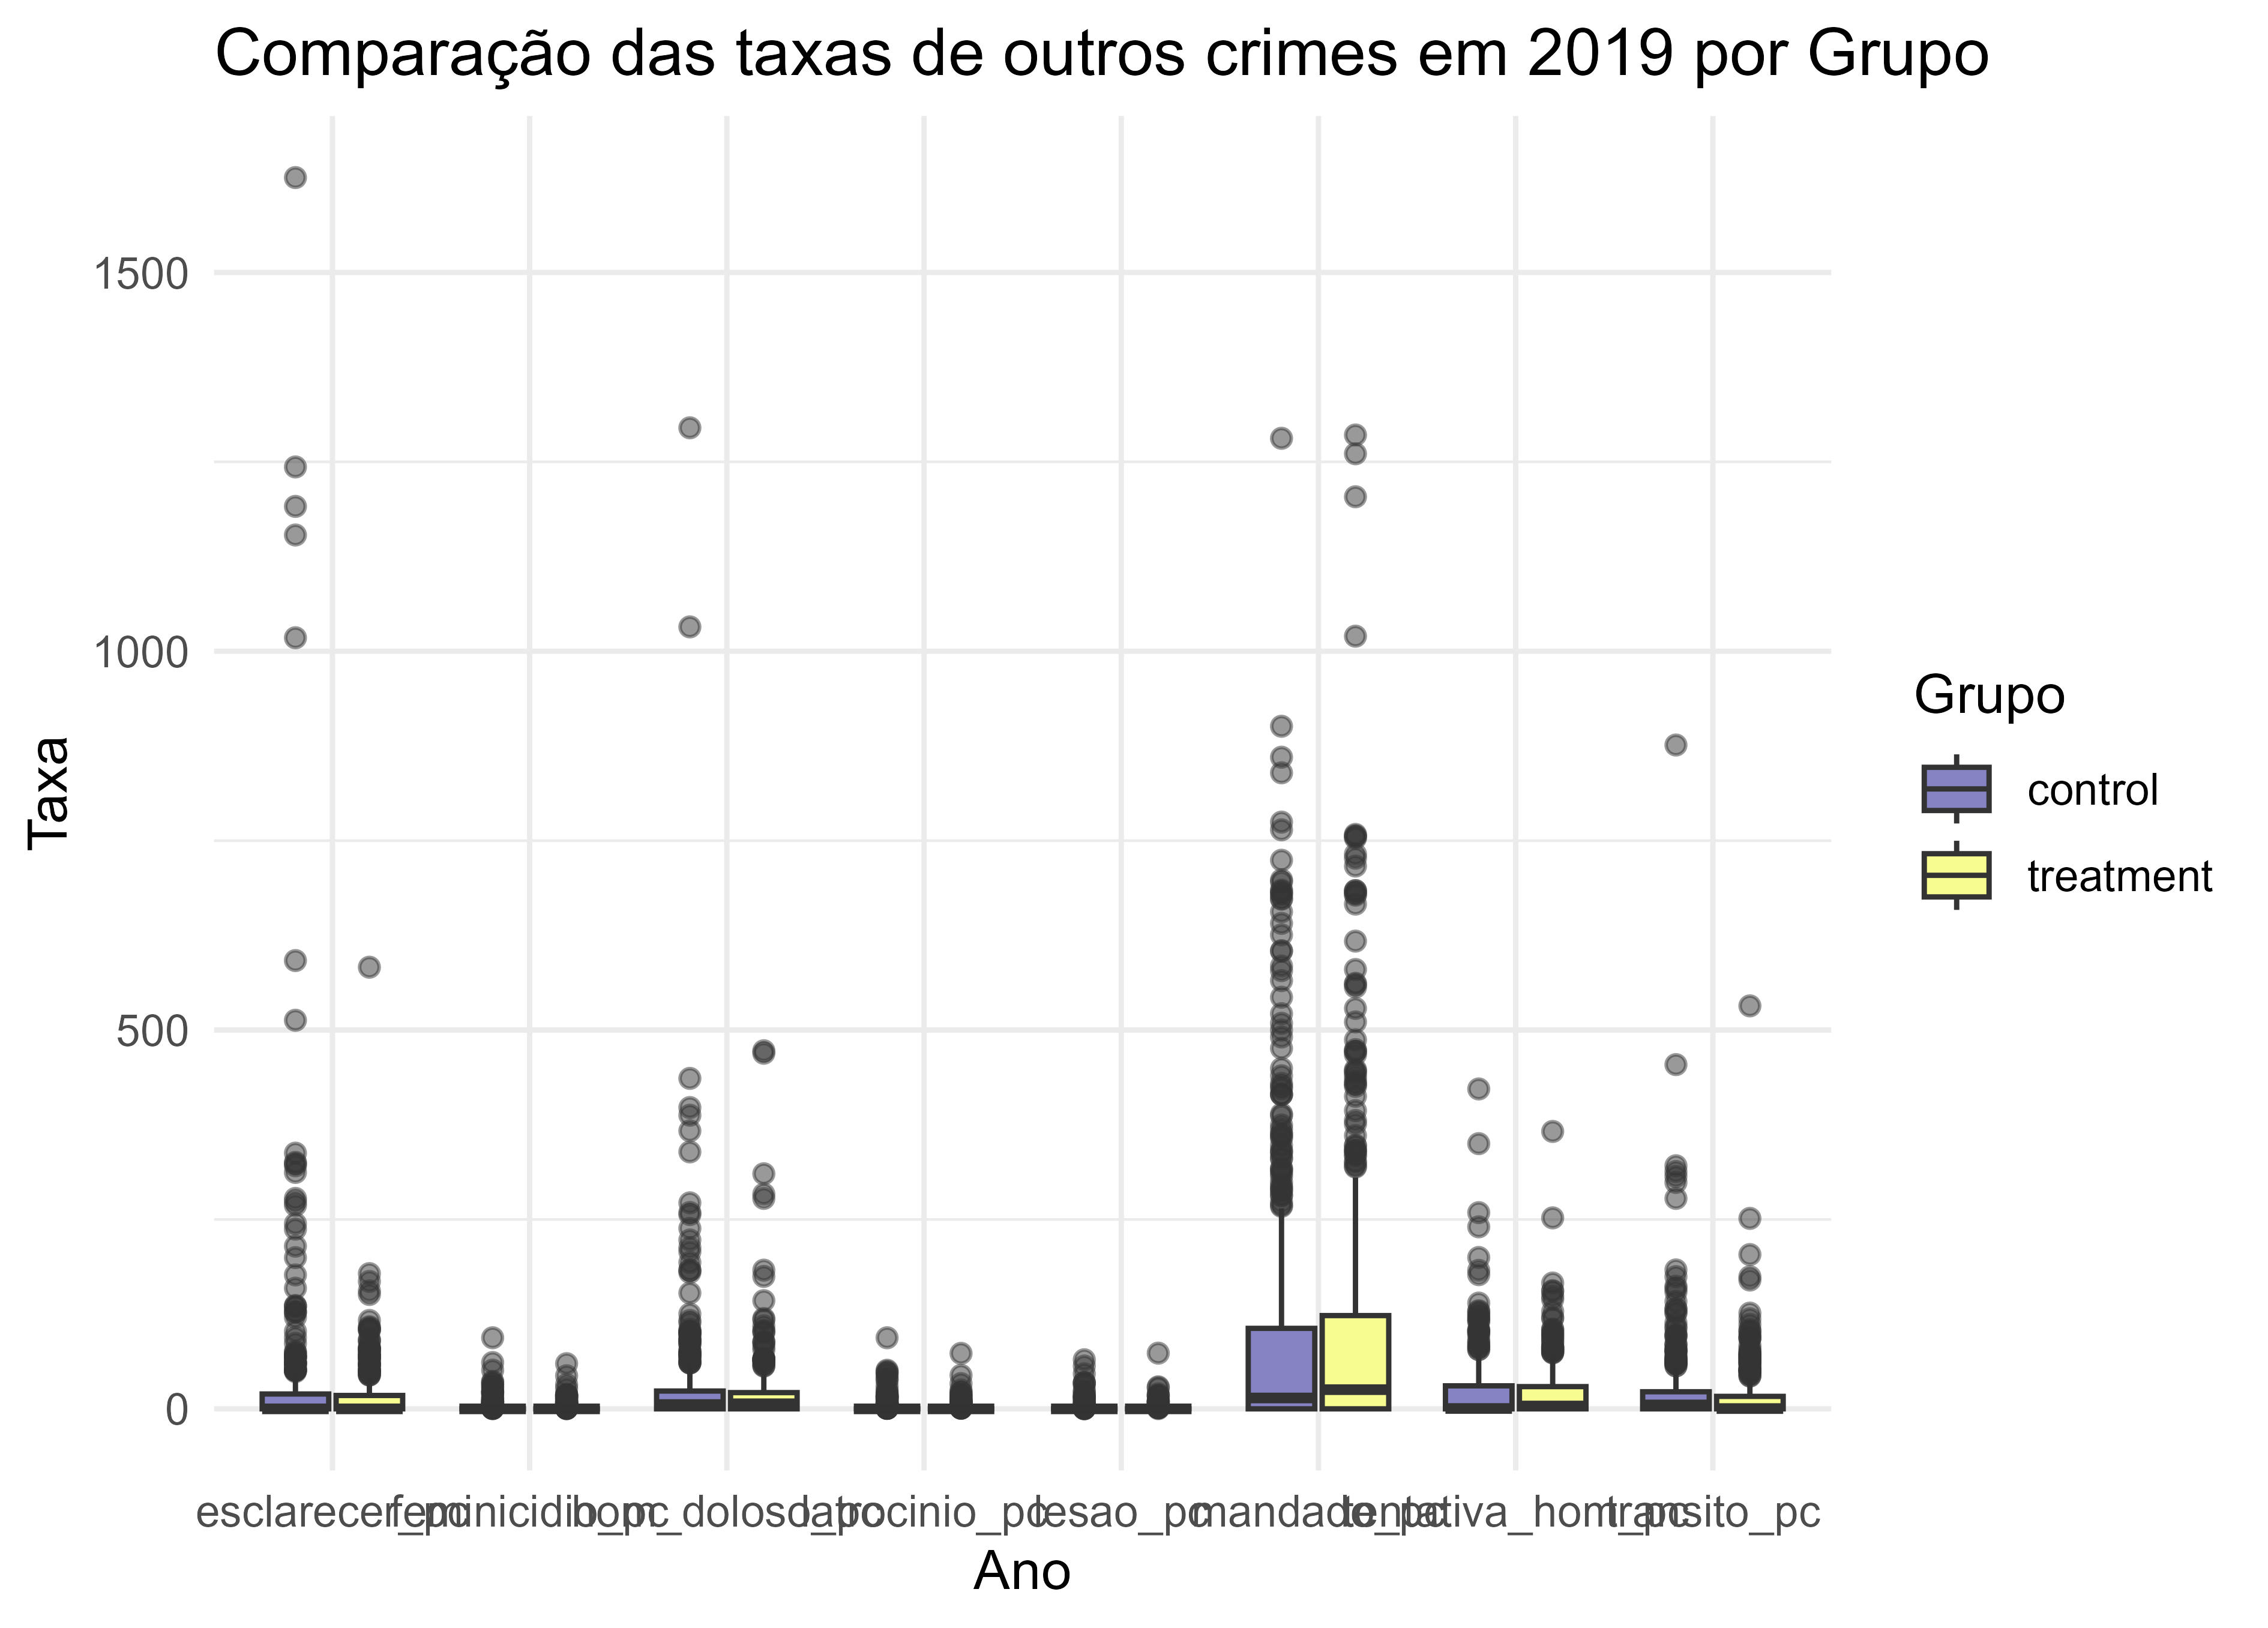
\includegraphics[width=1\linewidth]{figures/boxplot_outros}
		\label{fig:histoghom}
	\end{figure}
	
\end{frame}

\begin{frame}
	\begin{figure}
		\centering
		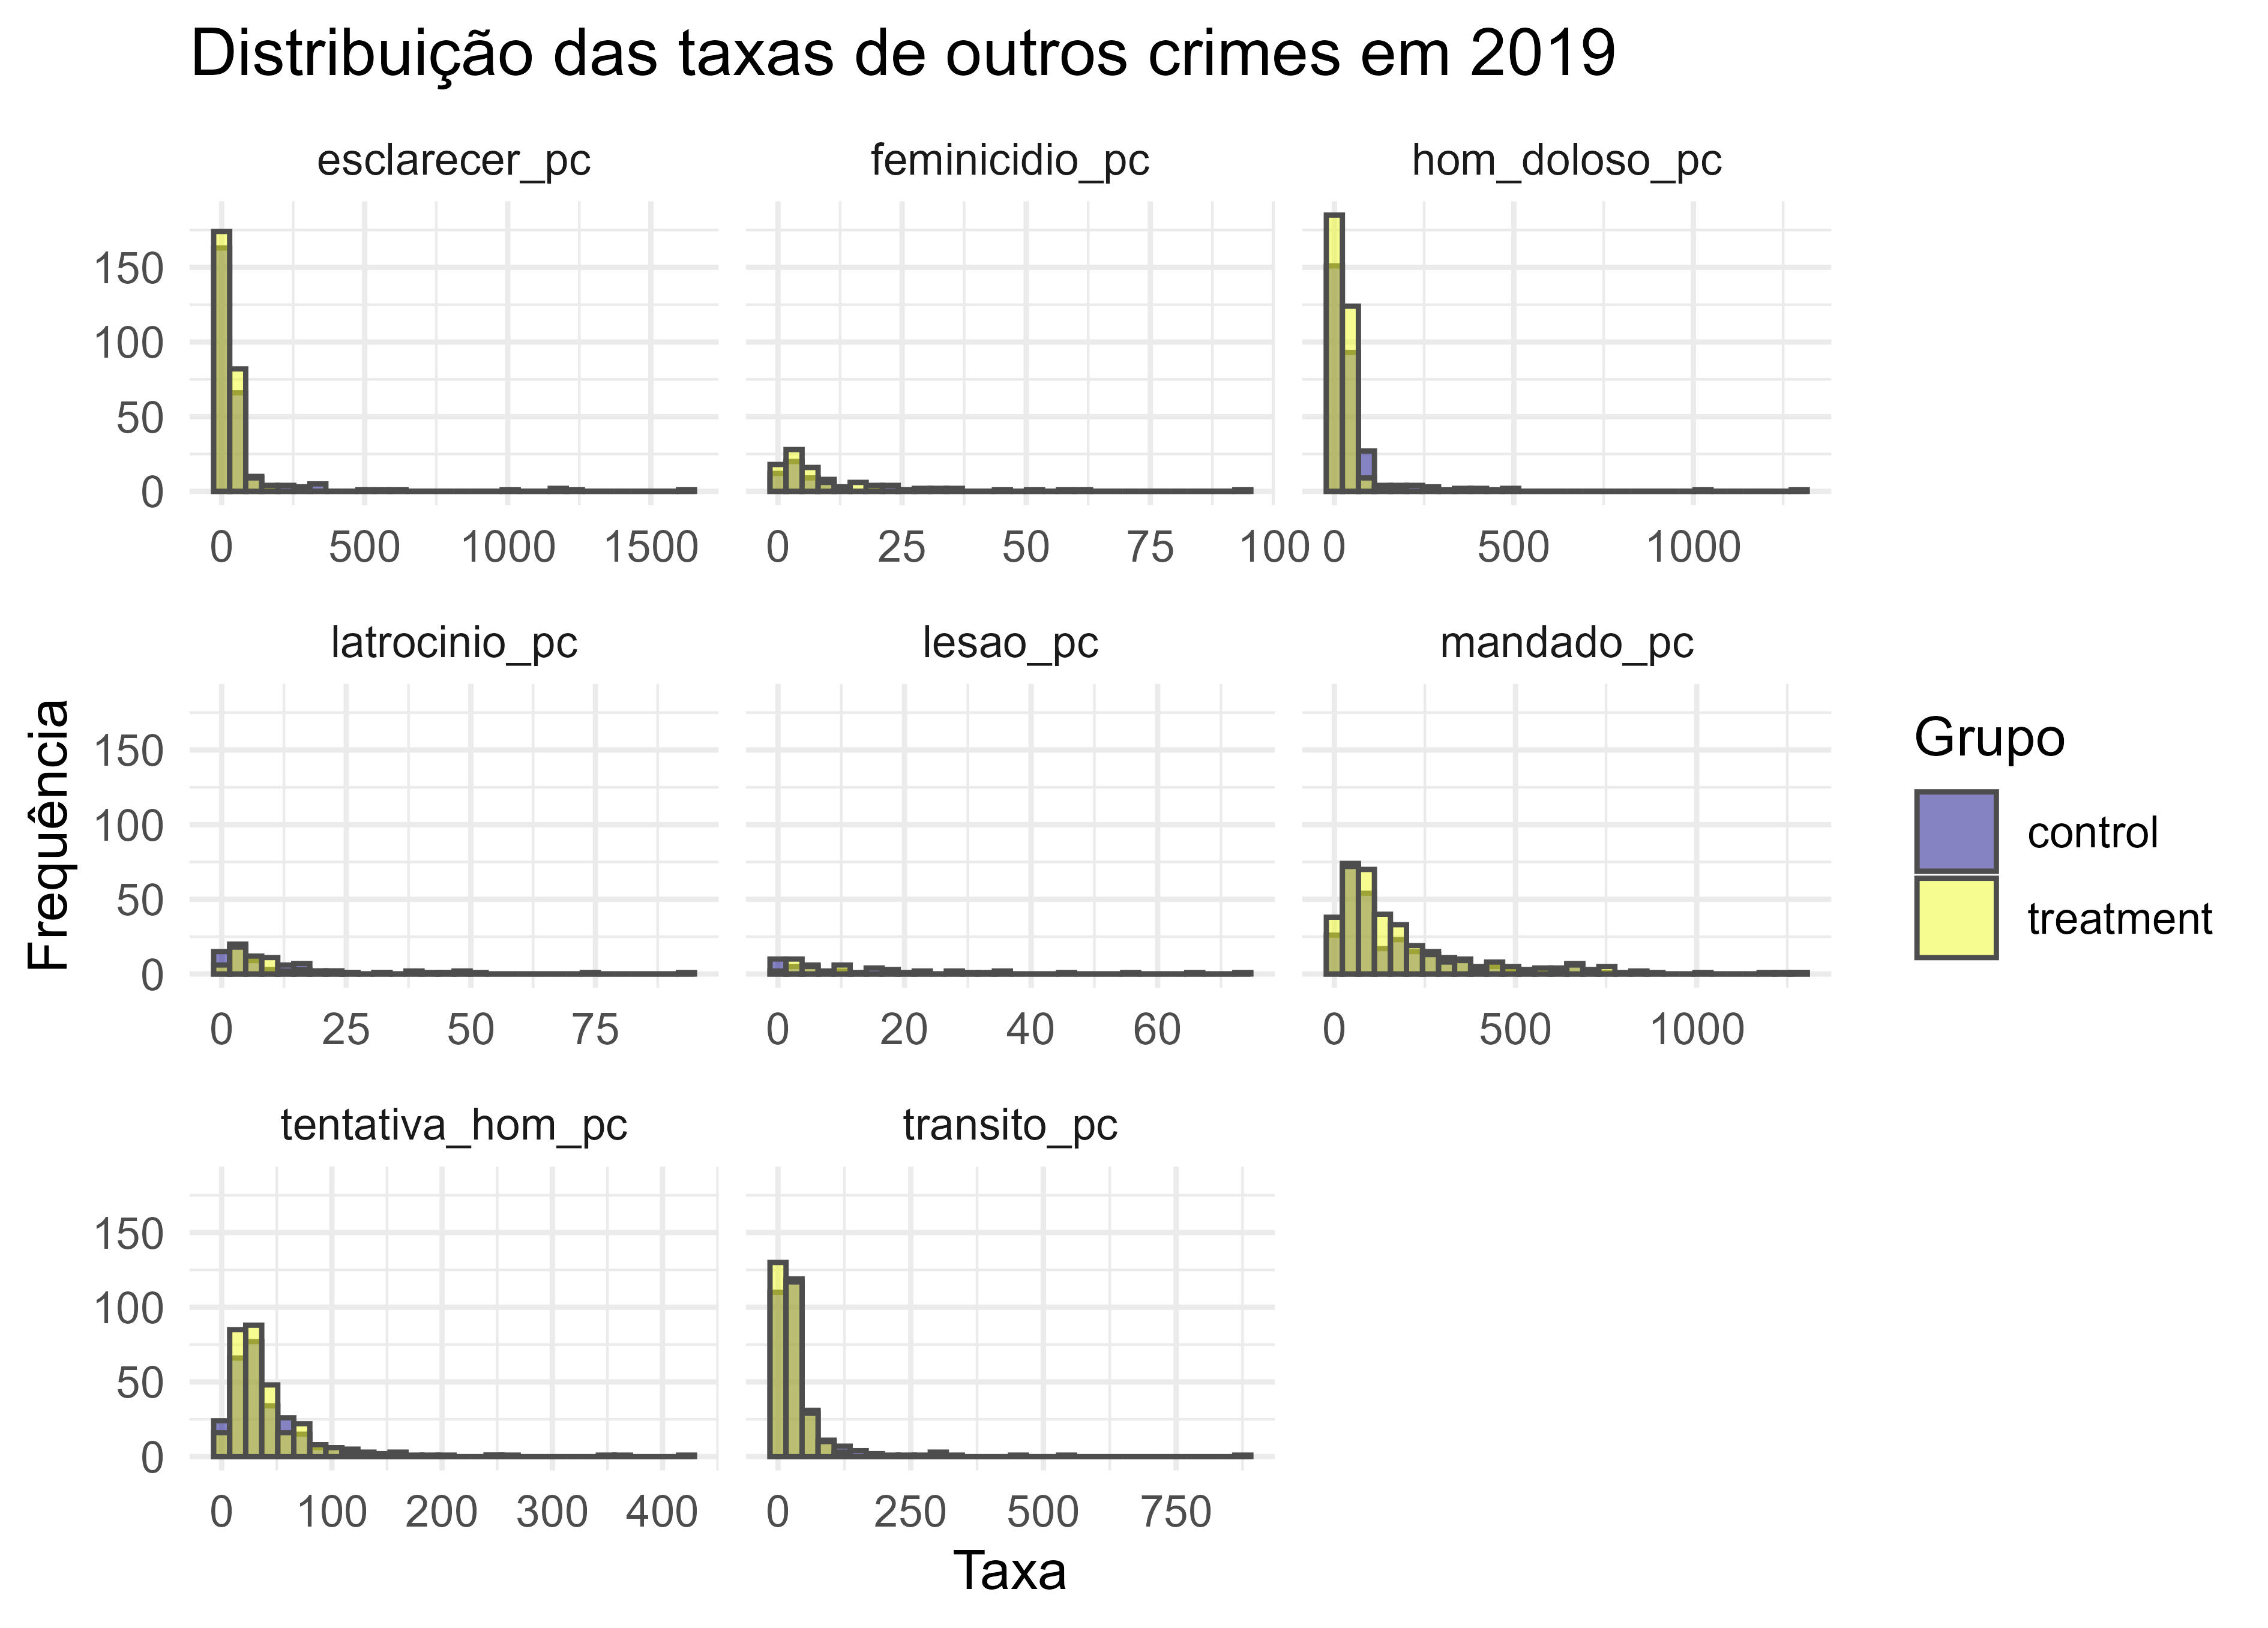
\includegraphics[width=1\linewidth]{figures/histog_outros_nonzero}
		\label{fig:histoghom}
	\end{figure}
	
\end{frame}

\begin{frame}
	\begin{figure}
		\centering
		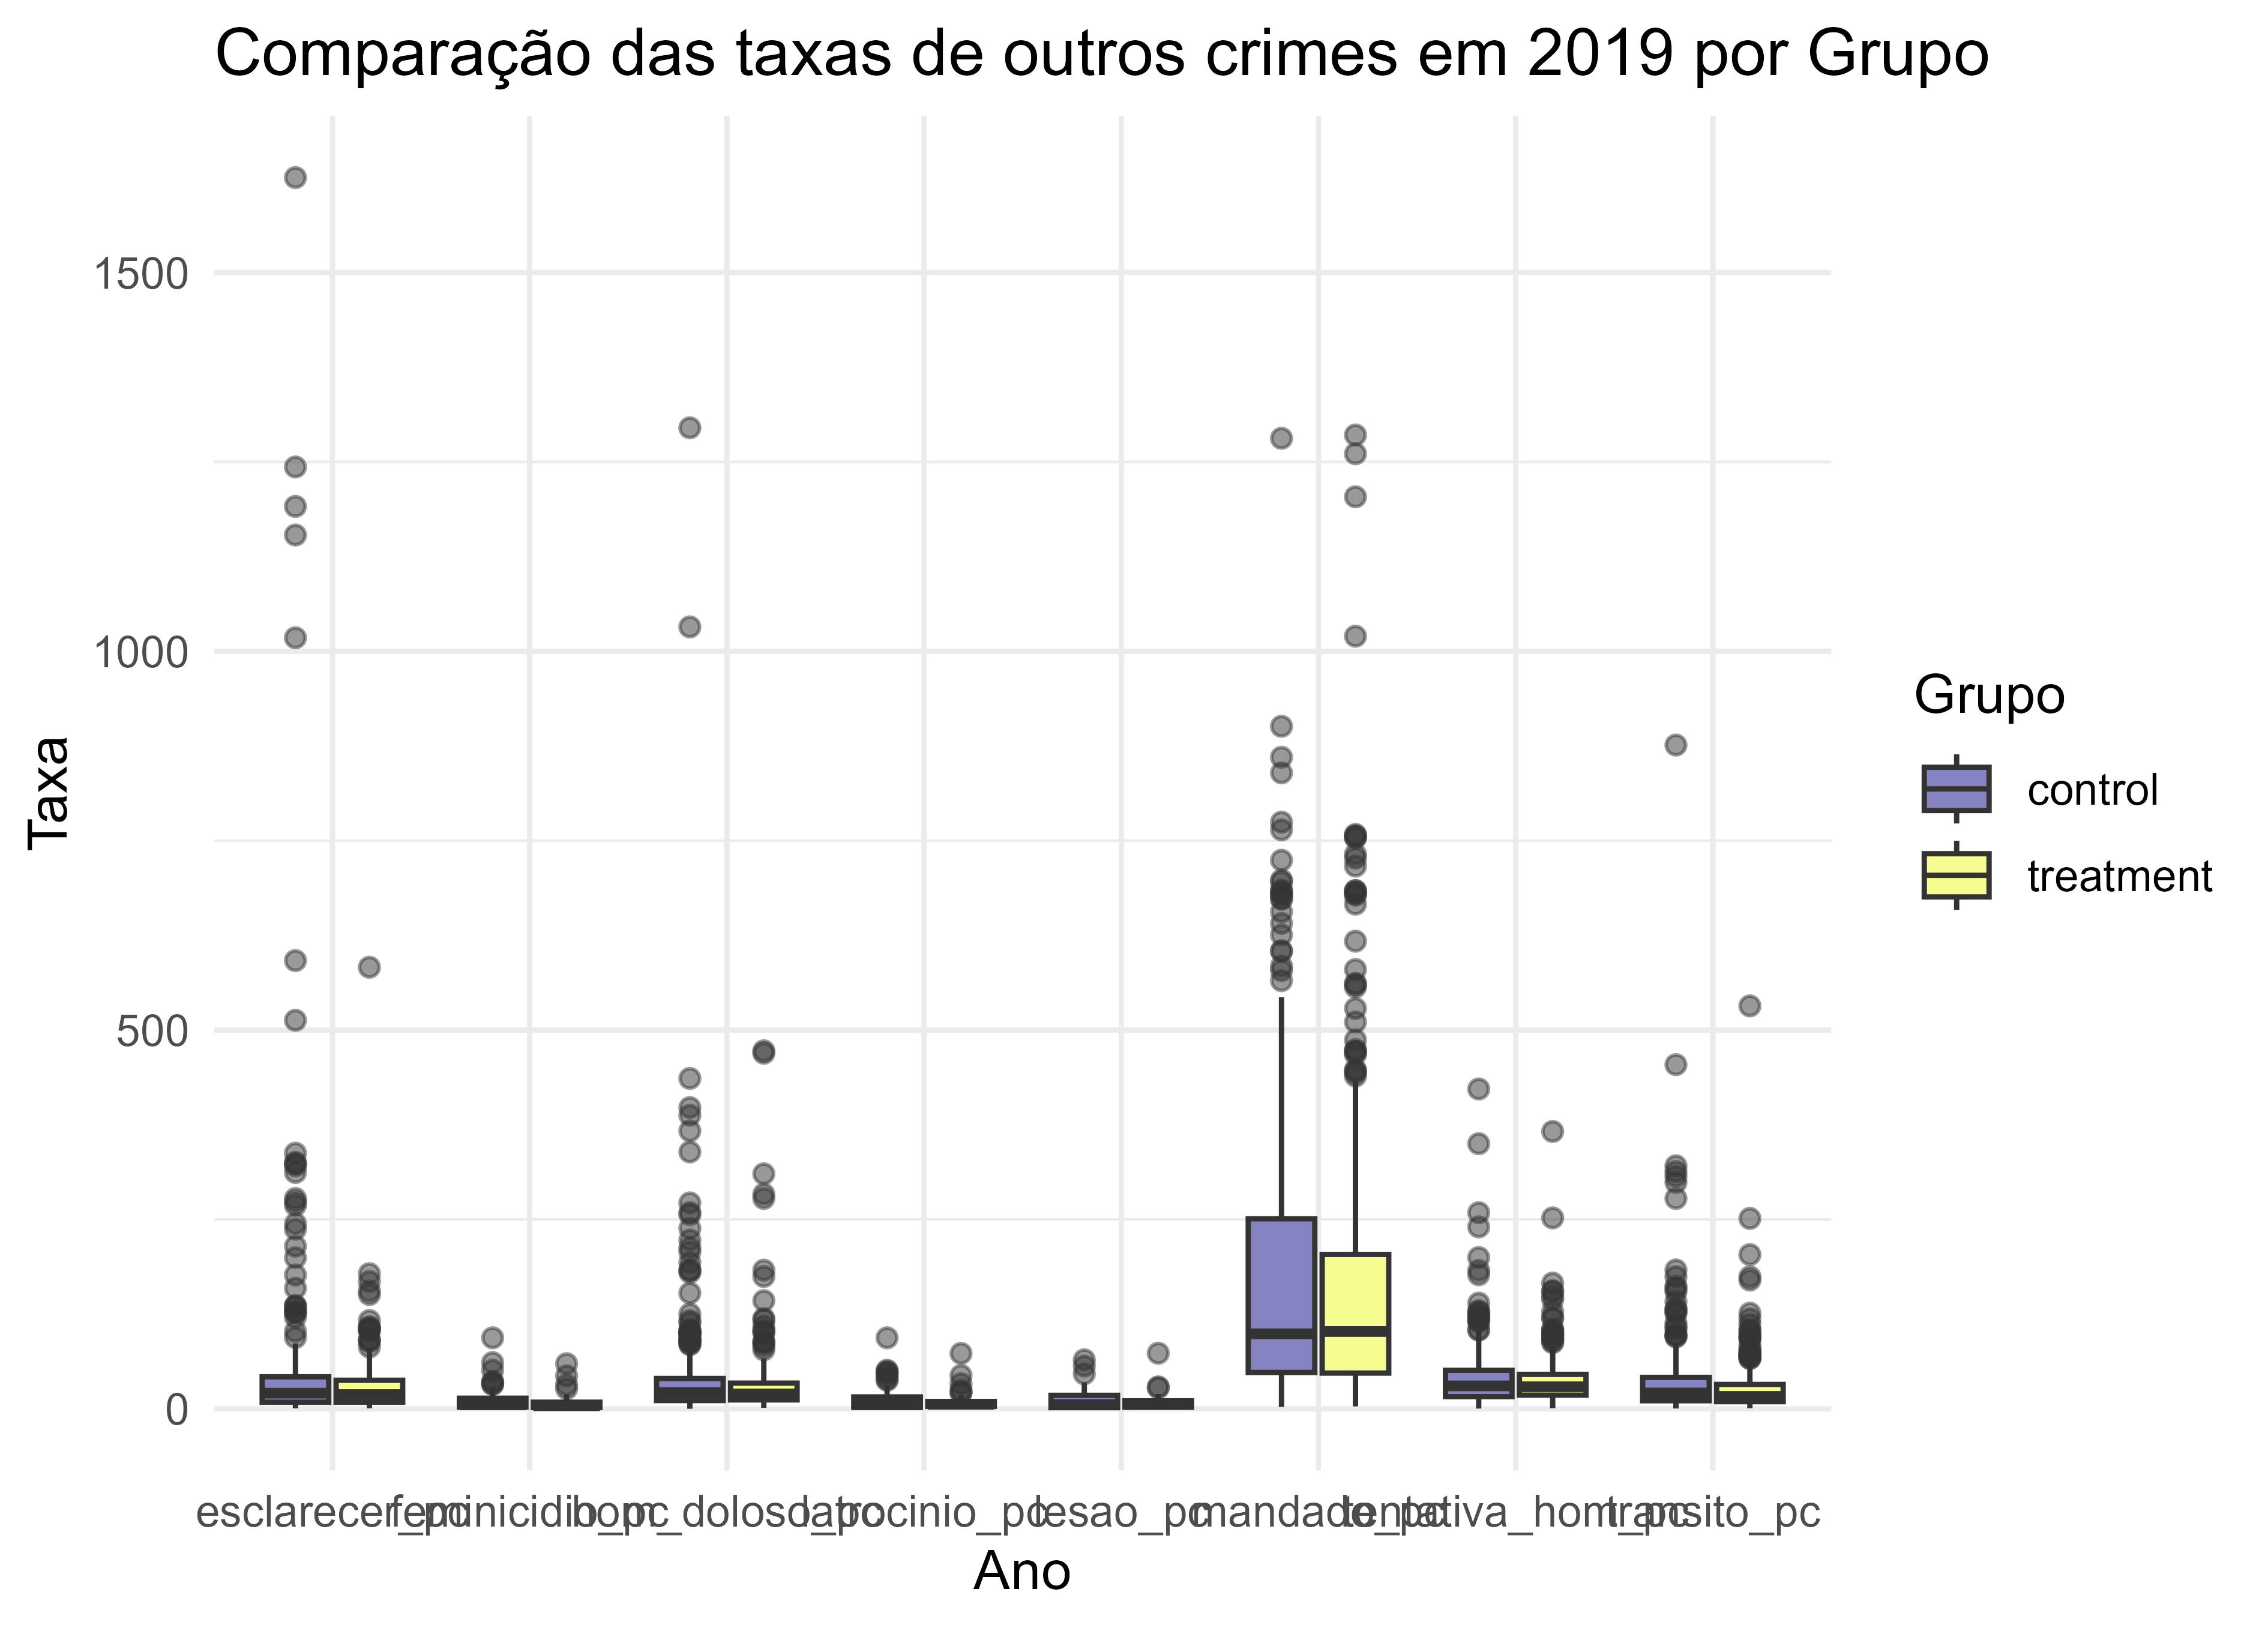
\includegraphics[width=1\linewidth]{figures/boxplot_outros_nonzero}
		\label{fig:histoghom}
	\end{figure}
\end{frame}

\begin{frame}
	\begin{figure}
		\centering
		\includegraphics[width=1\linewidth]{figures/mapa_feminicídios}
		\label{fig:histoghom}
	\end{figure}
\end{frame}

\begin{frame}
	\begin{figure}
		\centering
		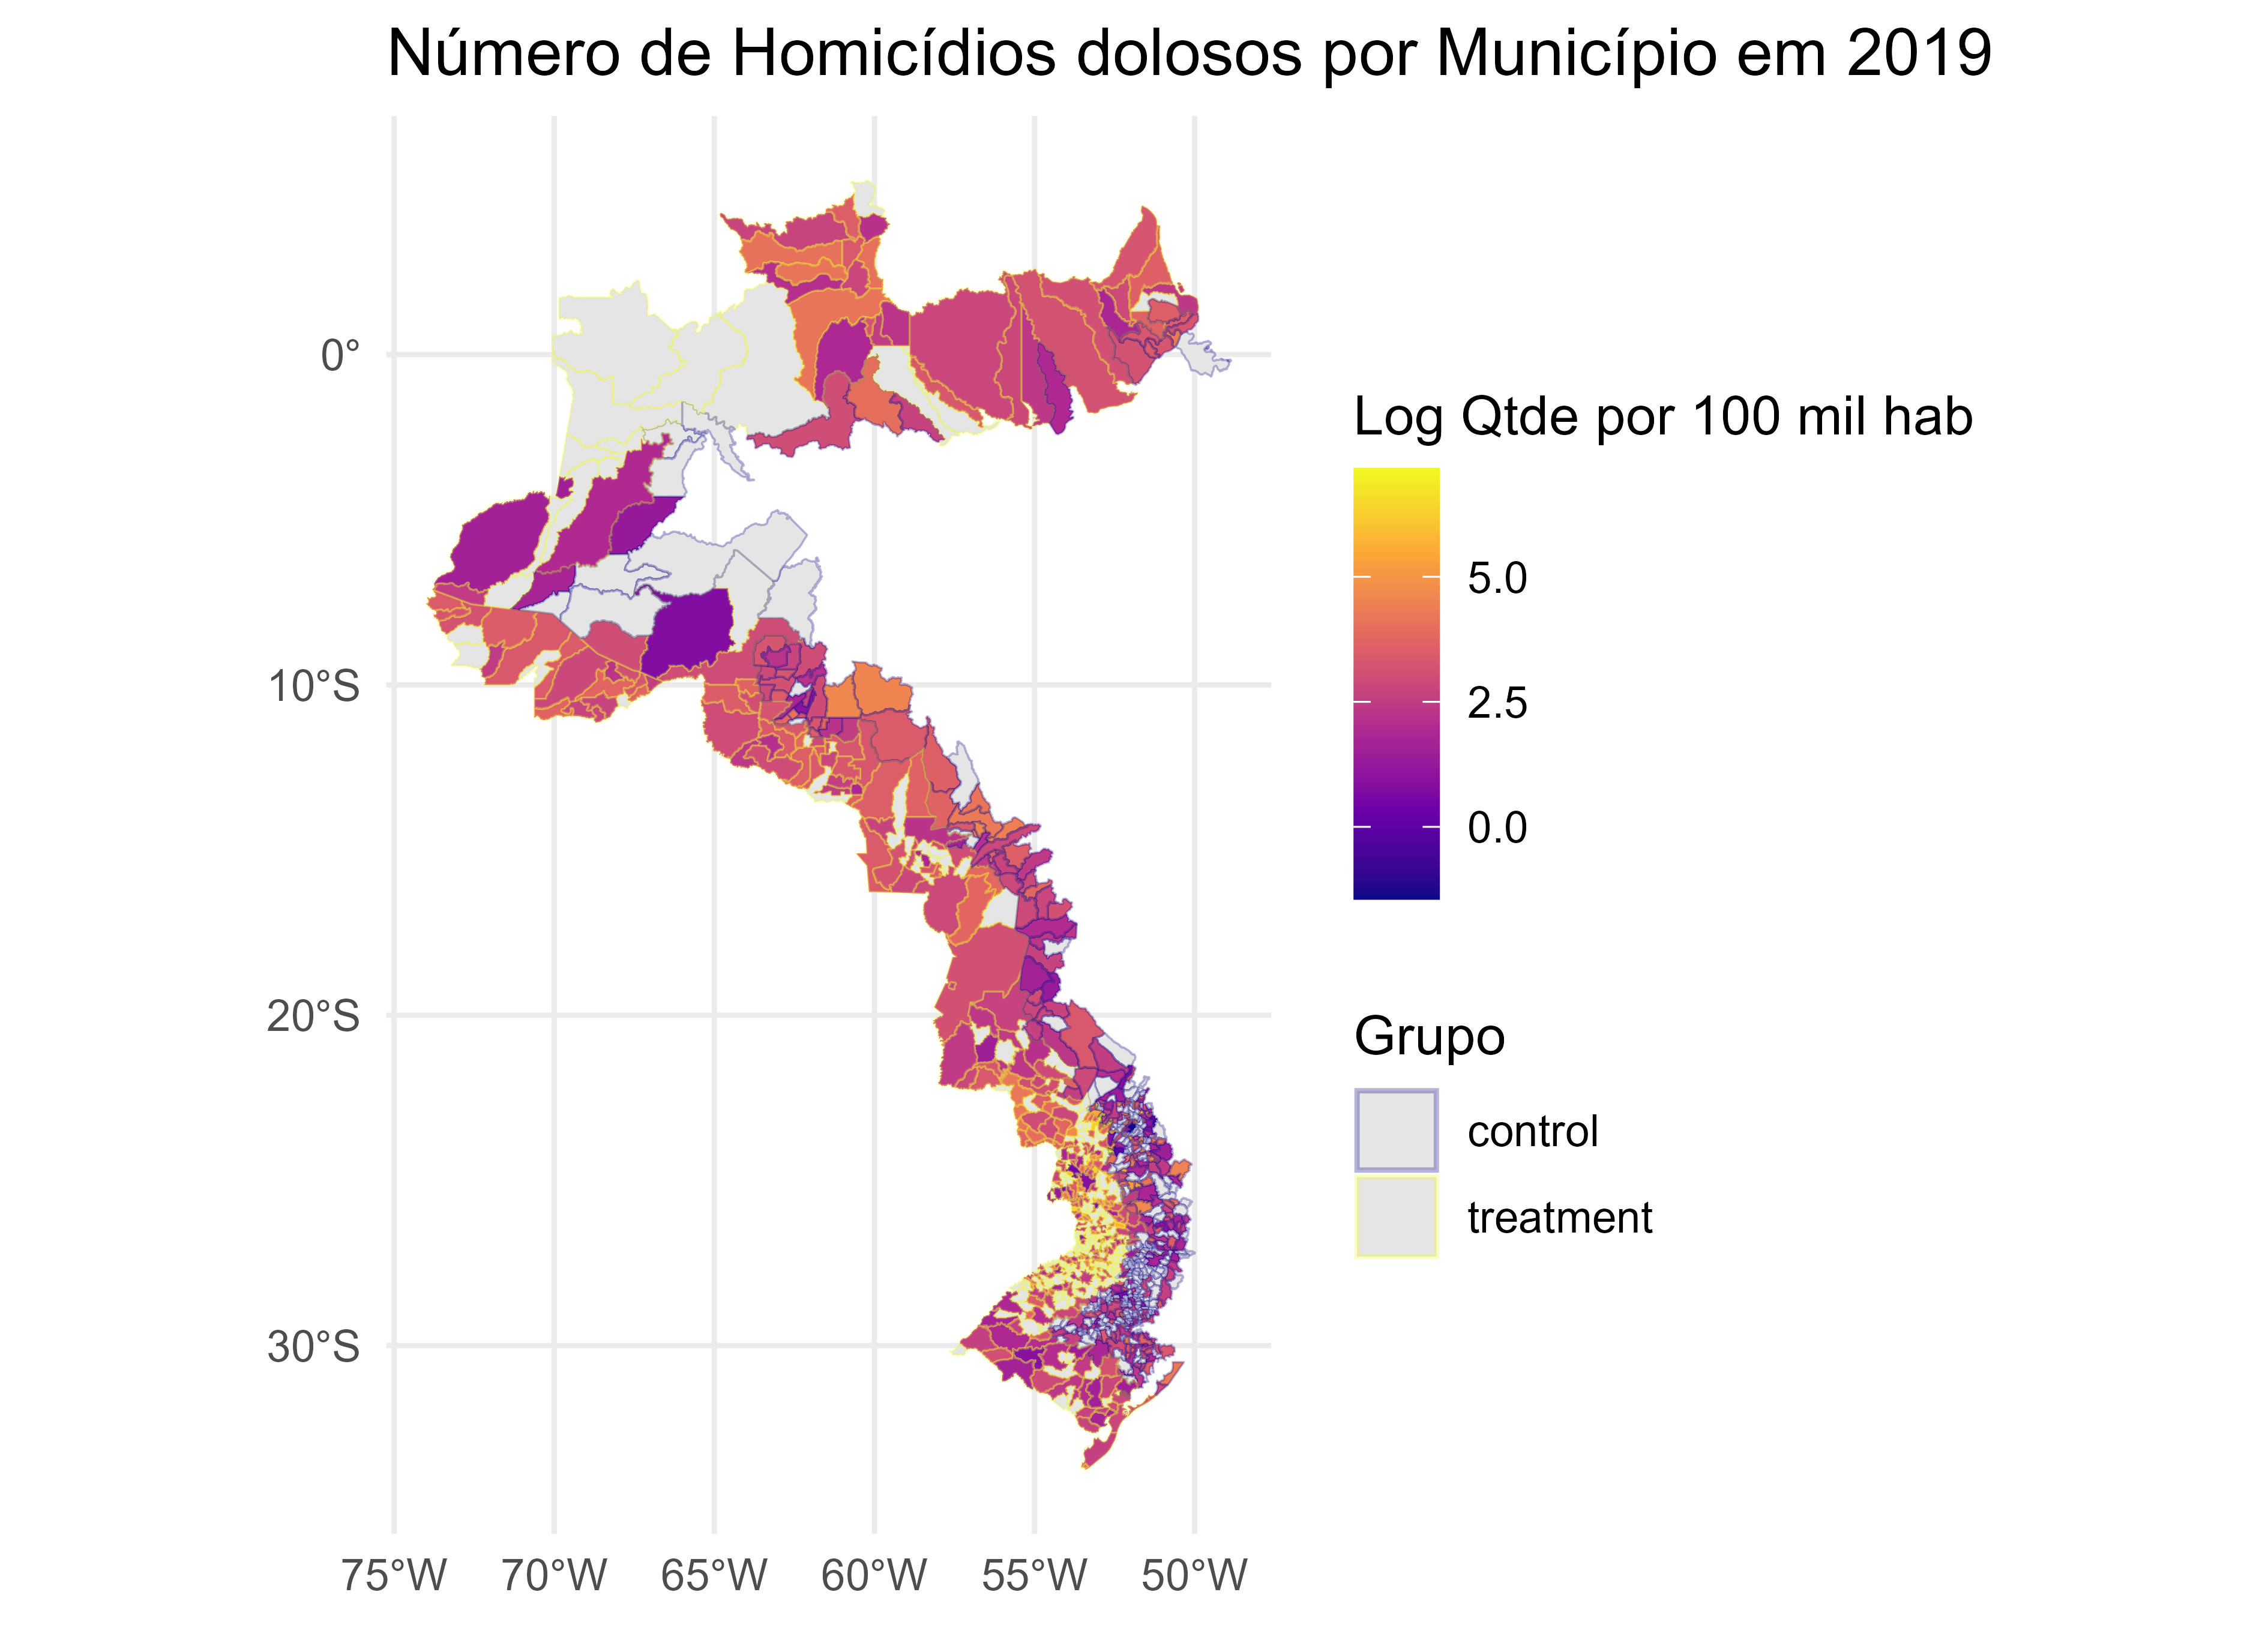
\includegraphics[width=1\linewidth]{figures/mapa_hom_dolosos}
		\label{fig:histoghom}
	\end{figure}
\end{frame}

\begin{frame}
	\begin{figure}
		\centering
		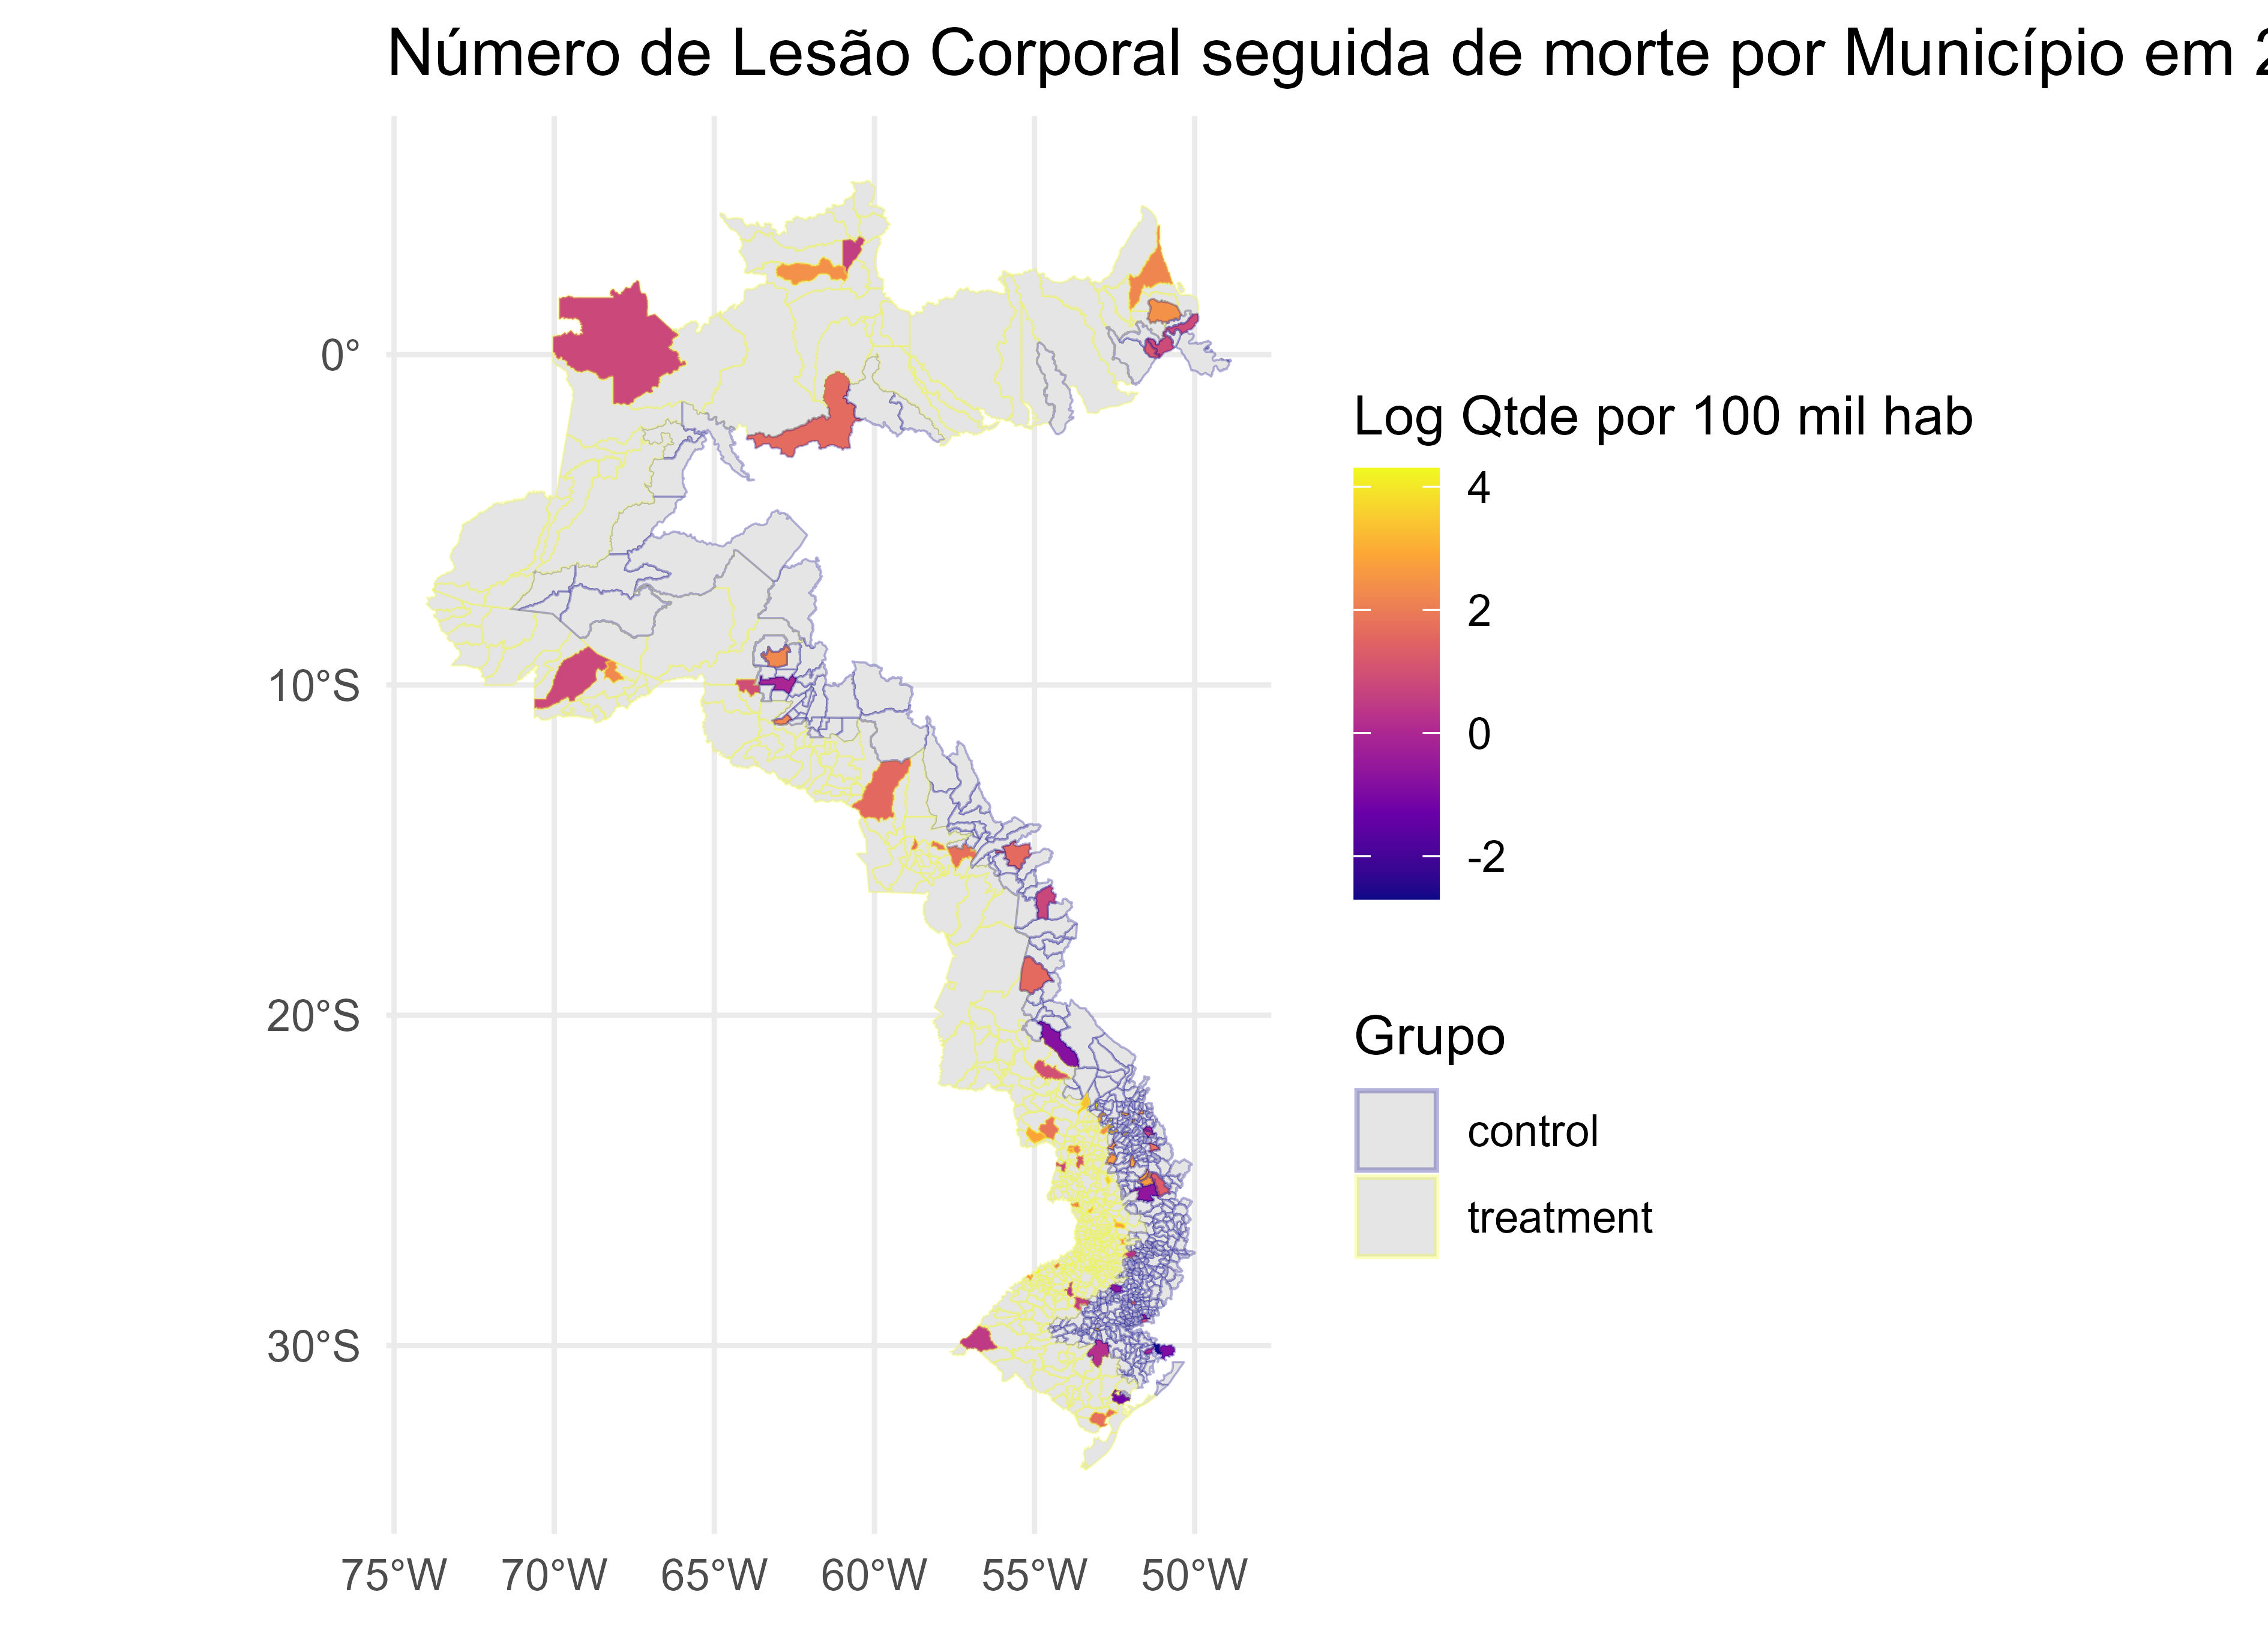
\includegraphics[width=1\linewidth]{figures/mapa_lesao}
		\label{fig:histoghom}
	\end{figure}
\end{frame}

\begin{frame}
	\begin{figure}
		\centering
		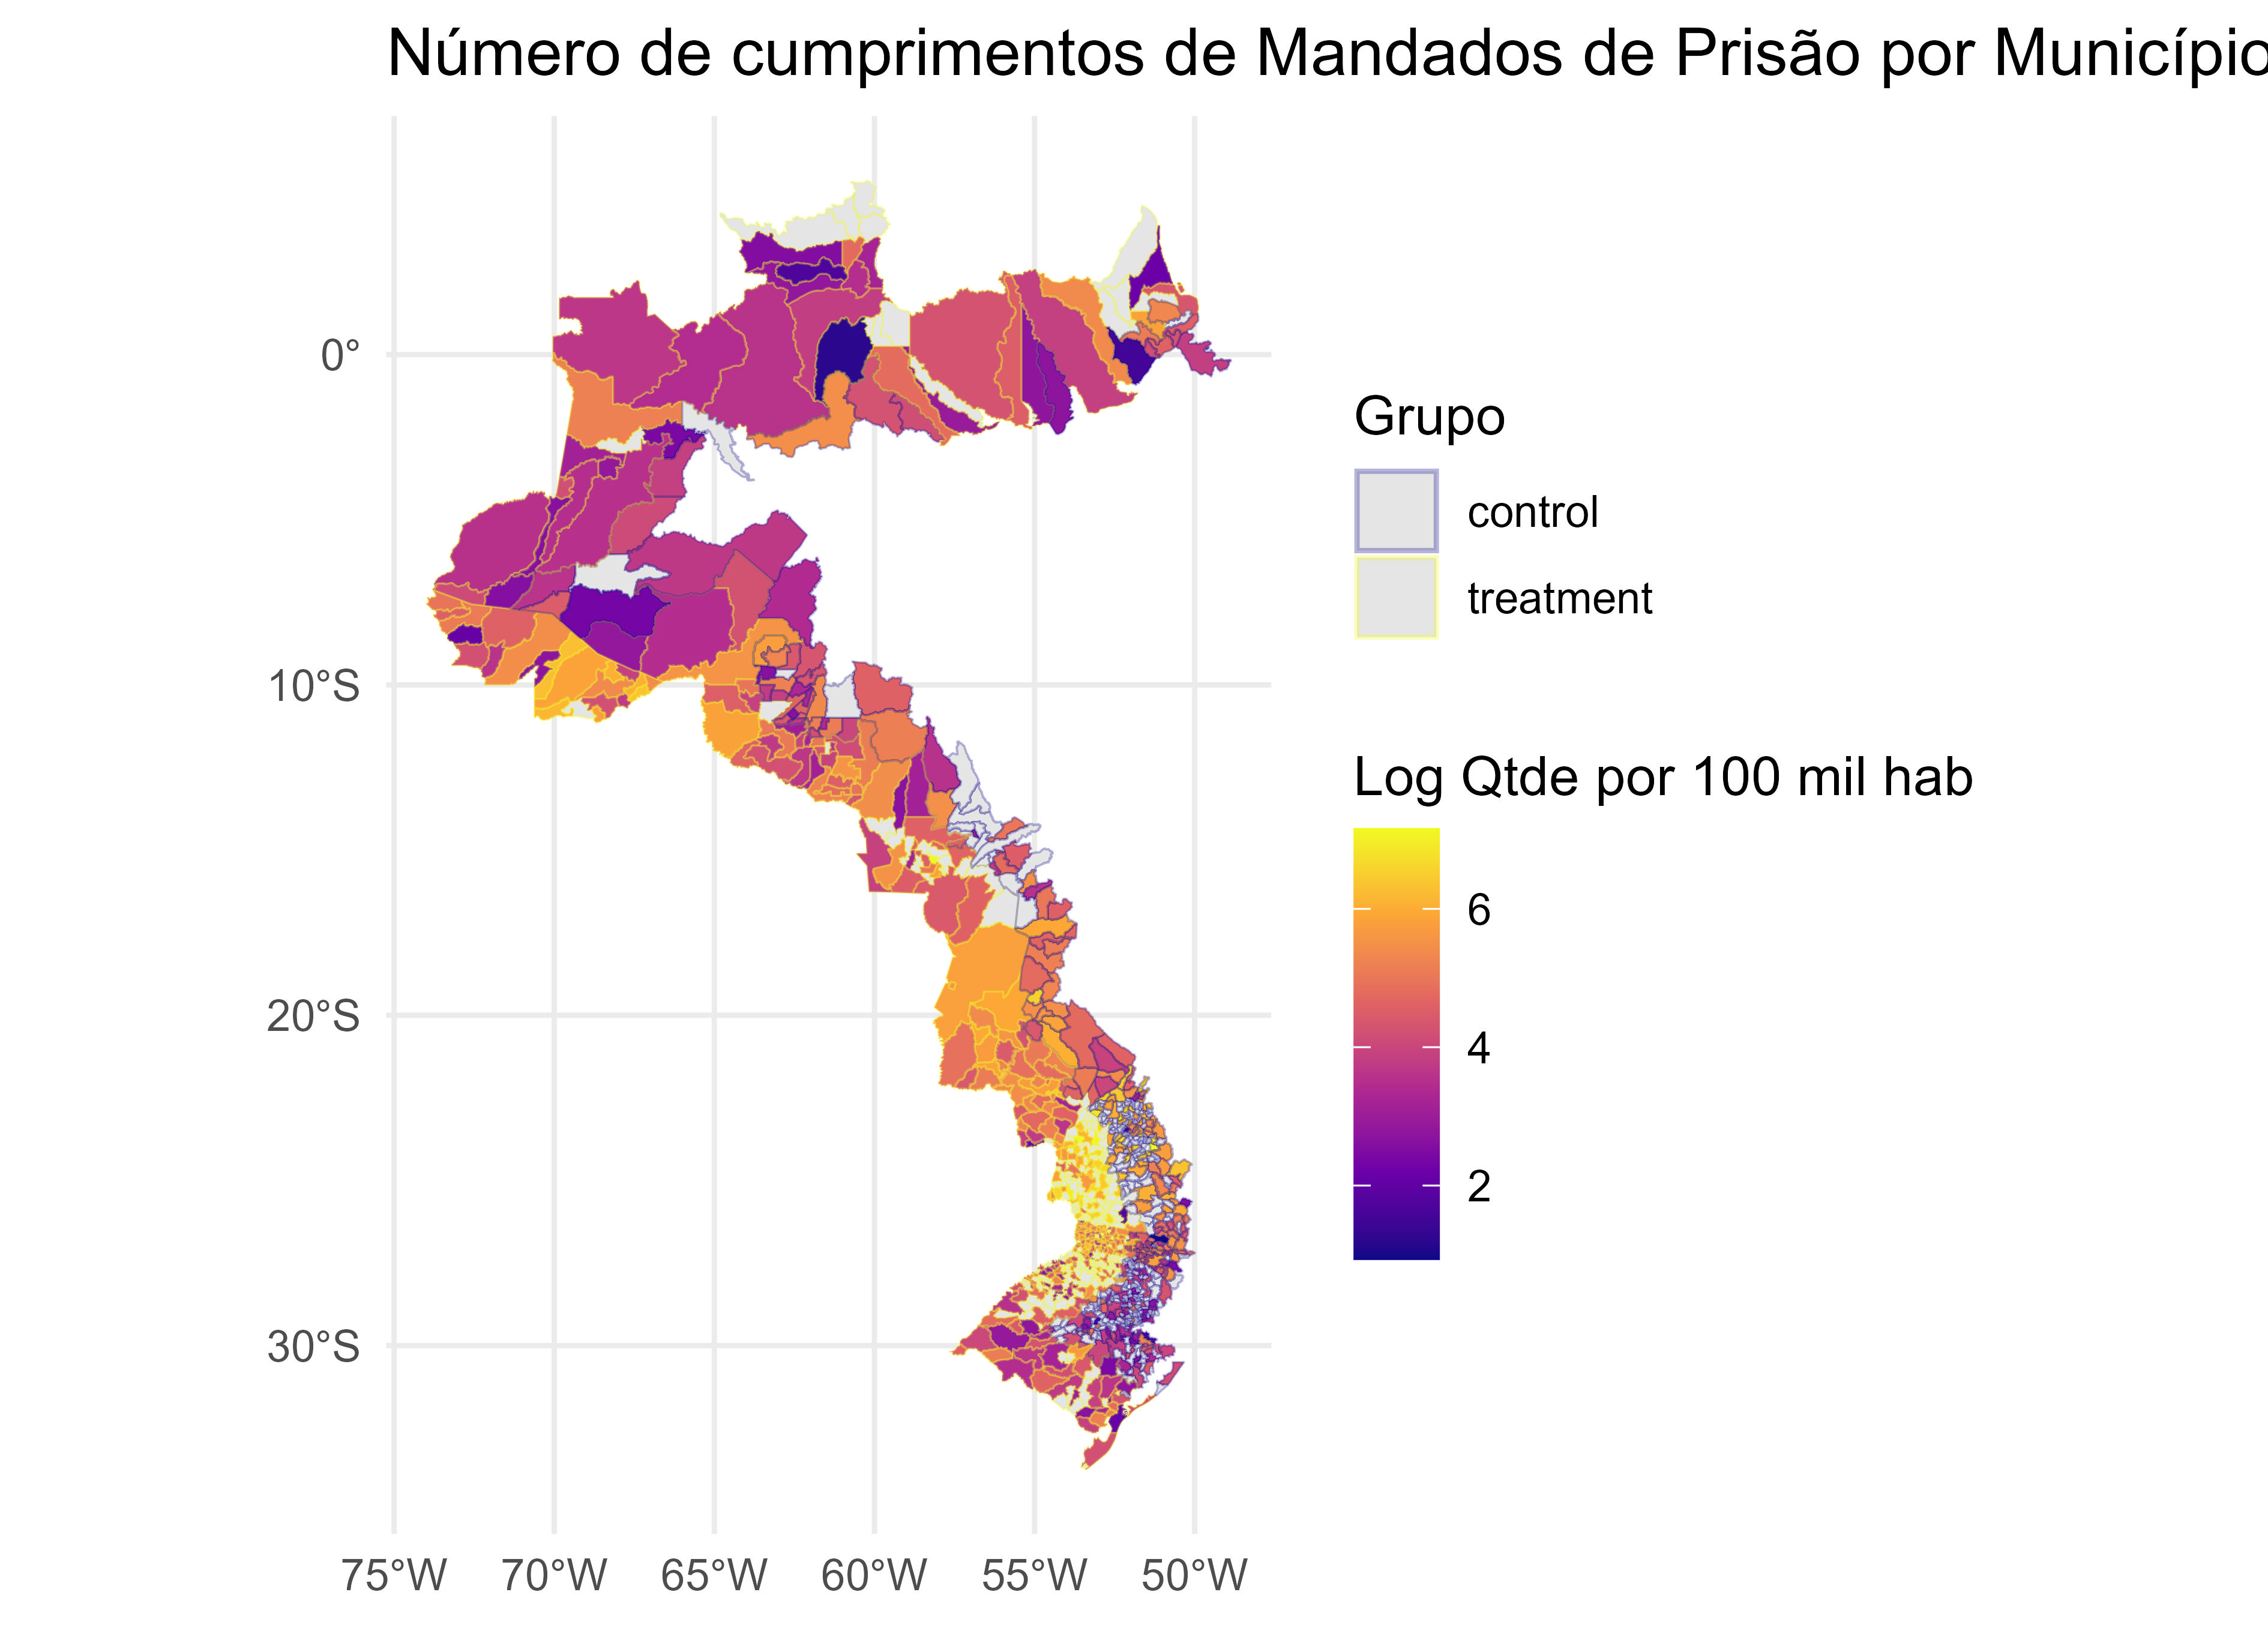
\includegraphics[width=1\linewidth]{figures/mapa_mandados}
		\label{fig:histoghom}
	\end{figure}
\end{frame}

\begin{frame}
	\begin{figure}
		\centering
		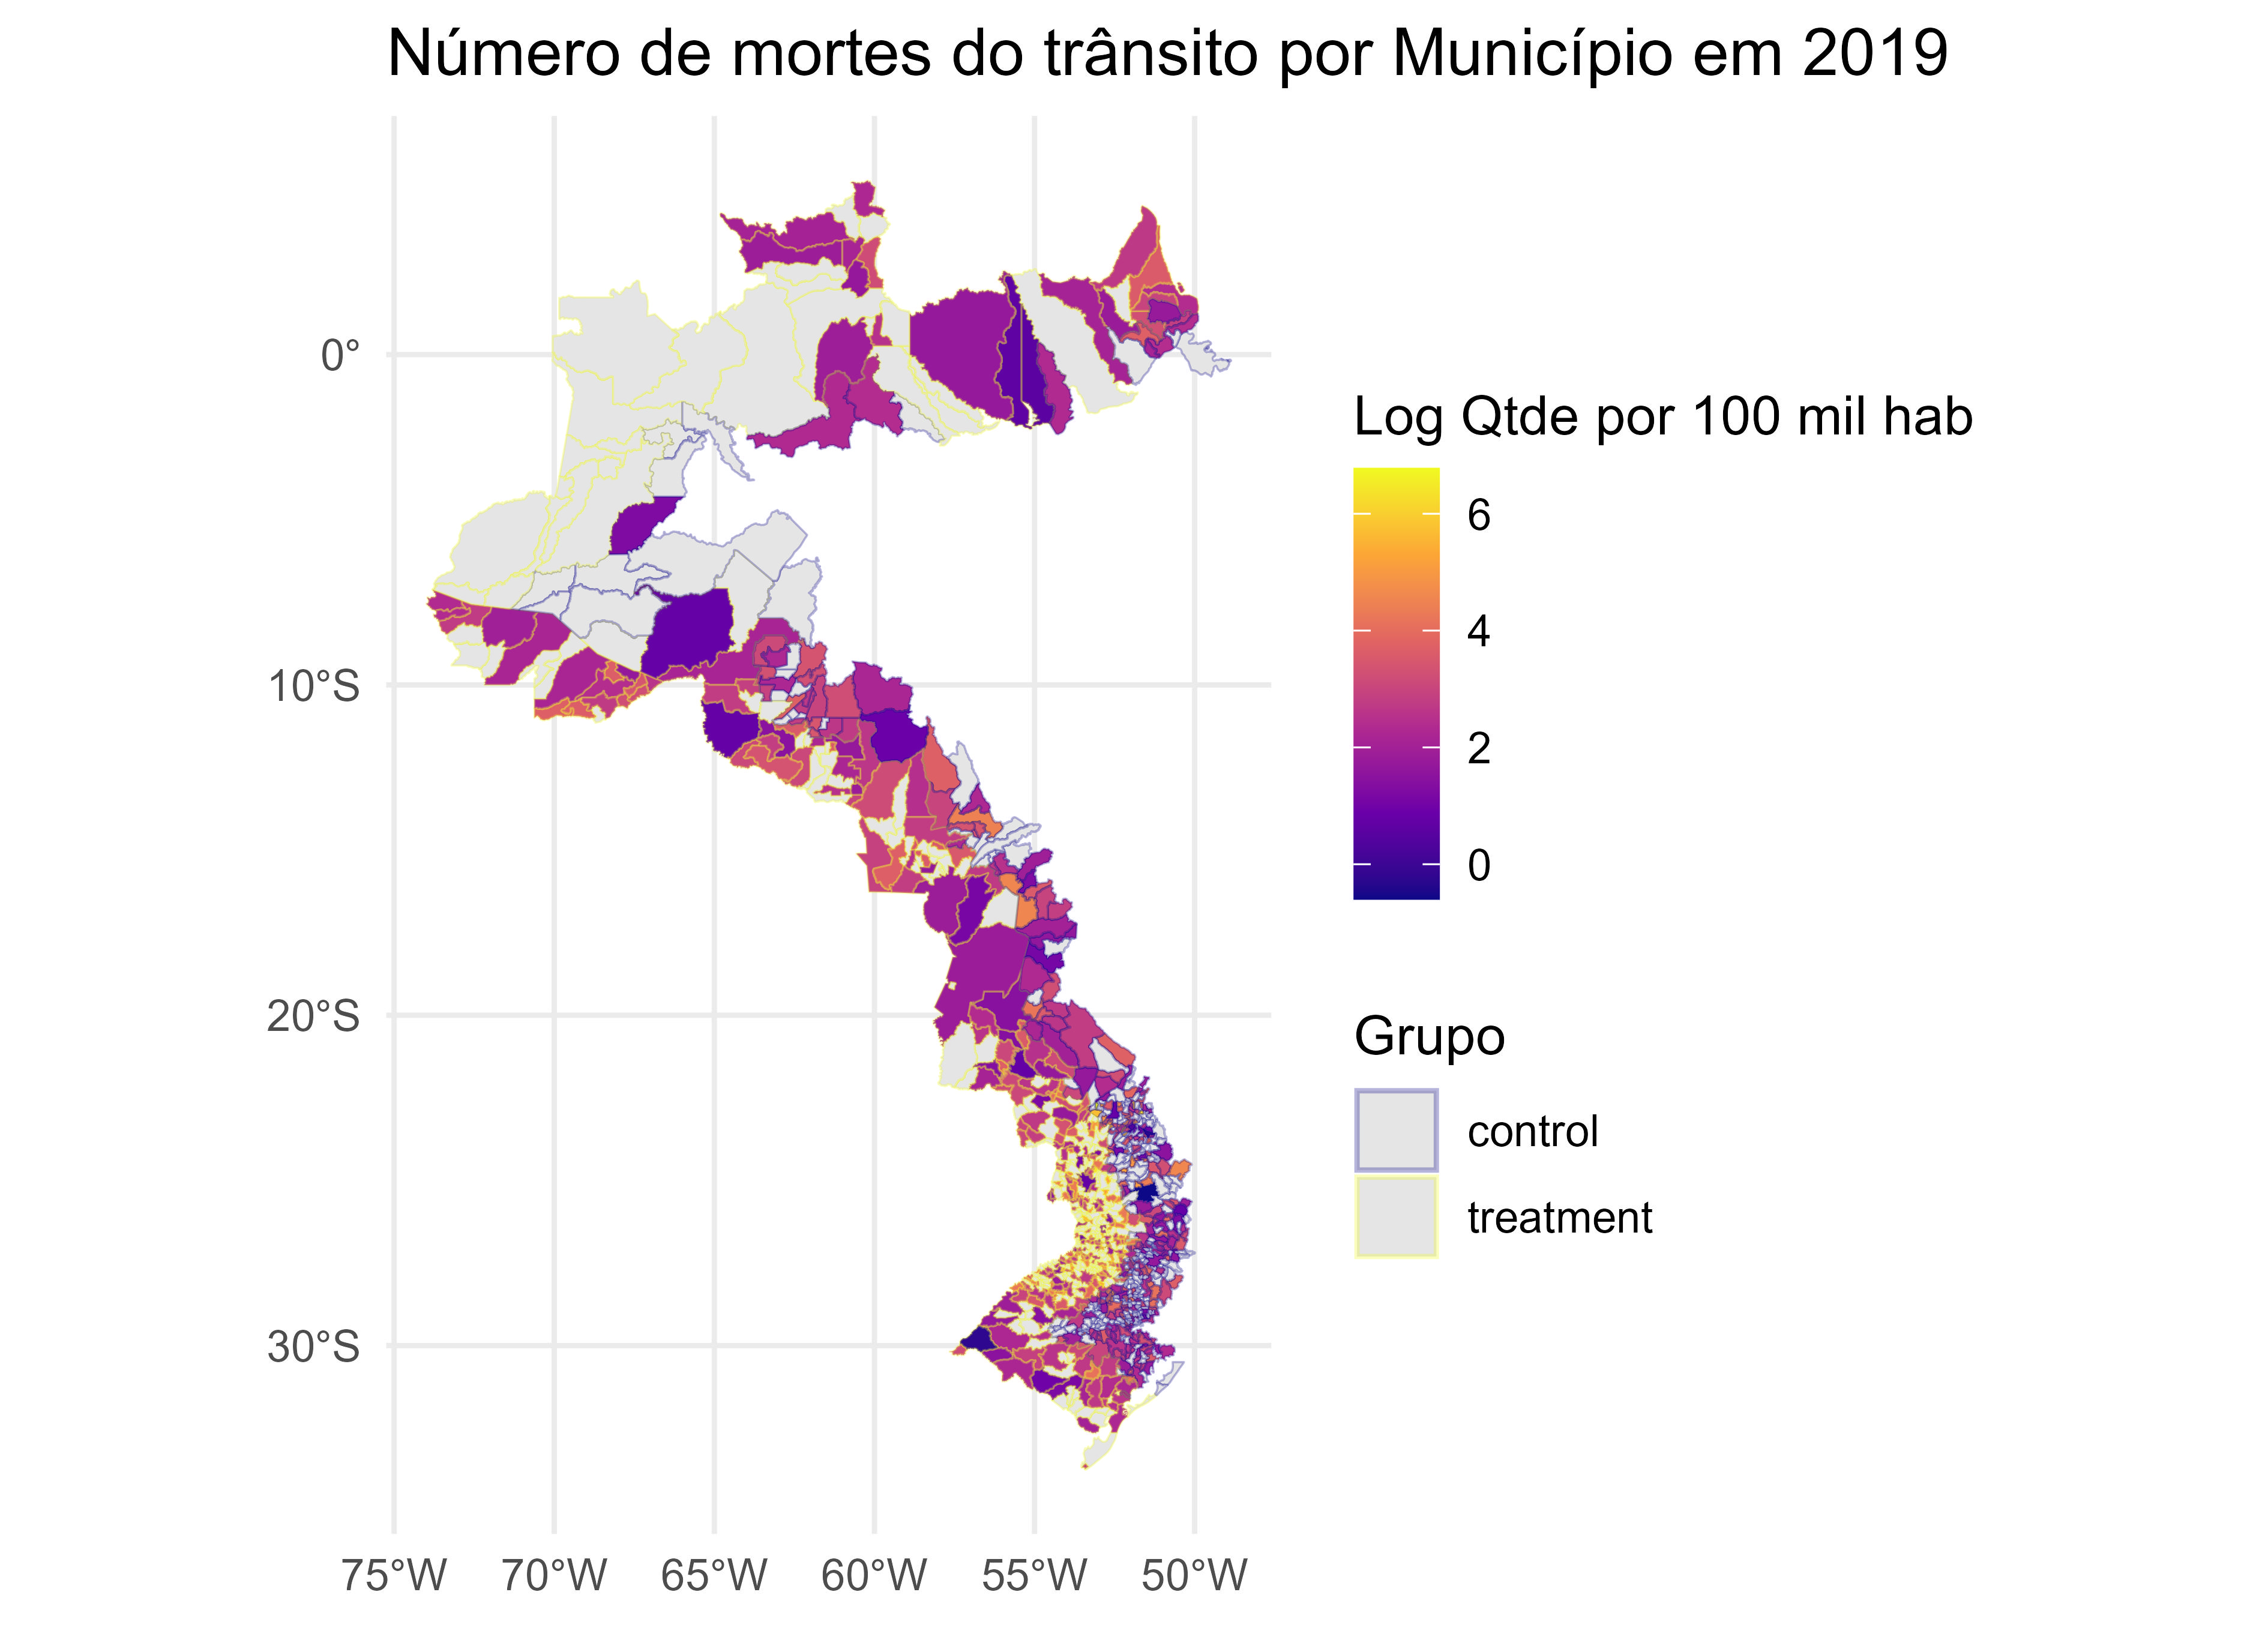
\includegraphics[width=1\linewidth]{figures/mapa_transito}
		\label{fig:histoghom}
	\end{figure}
\end{frame}

\begin{frame}
	\begin{figure}
		\centering
		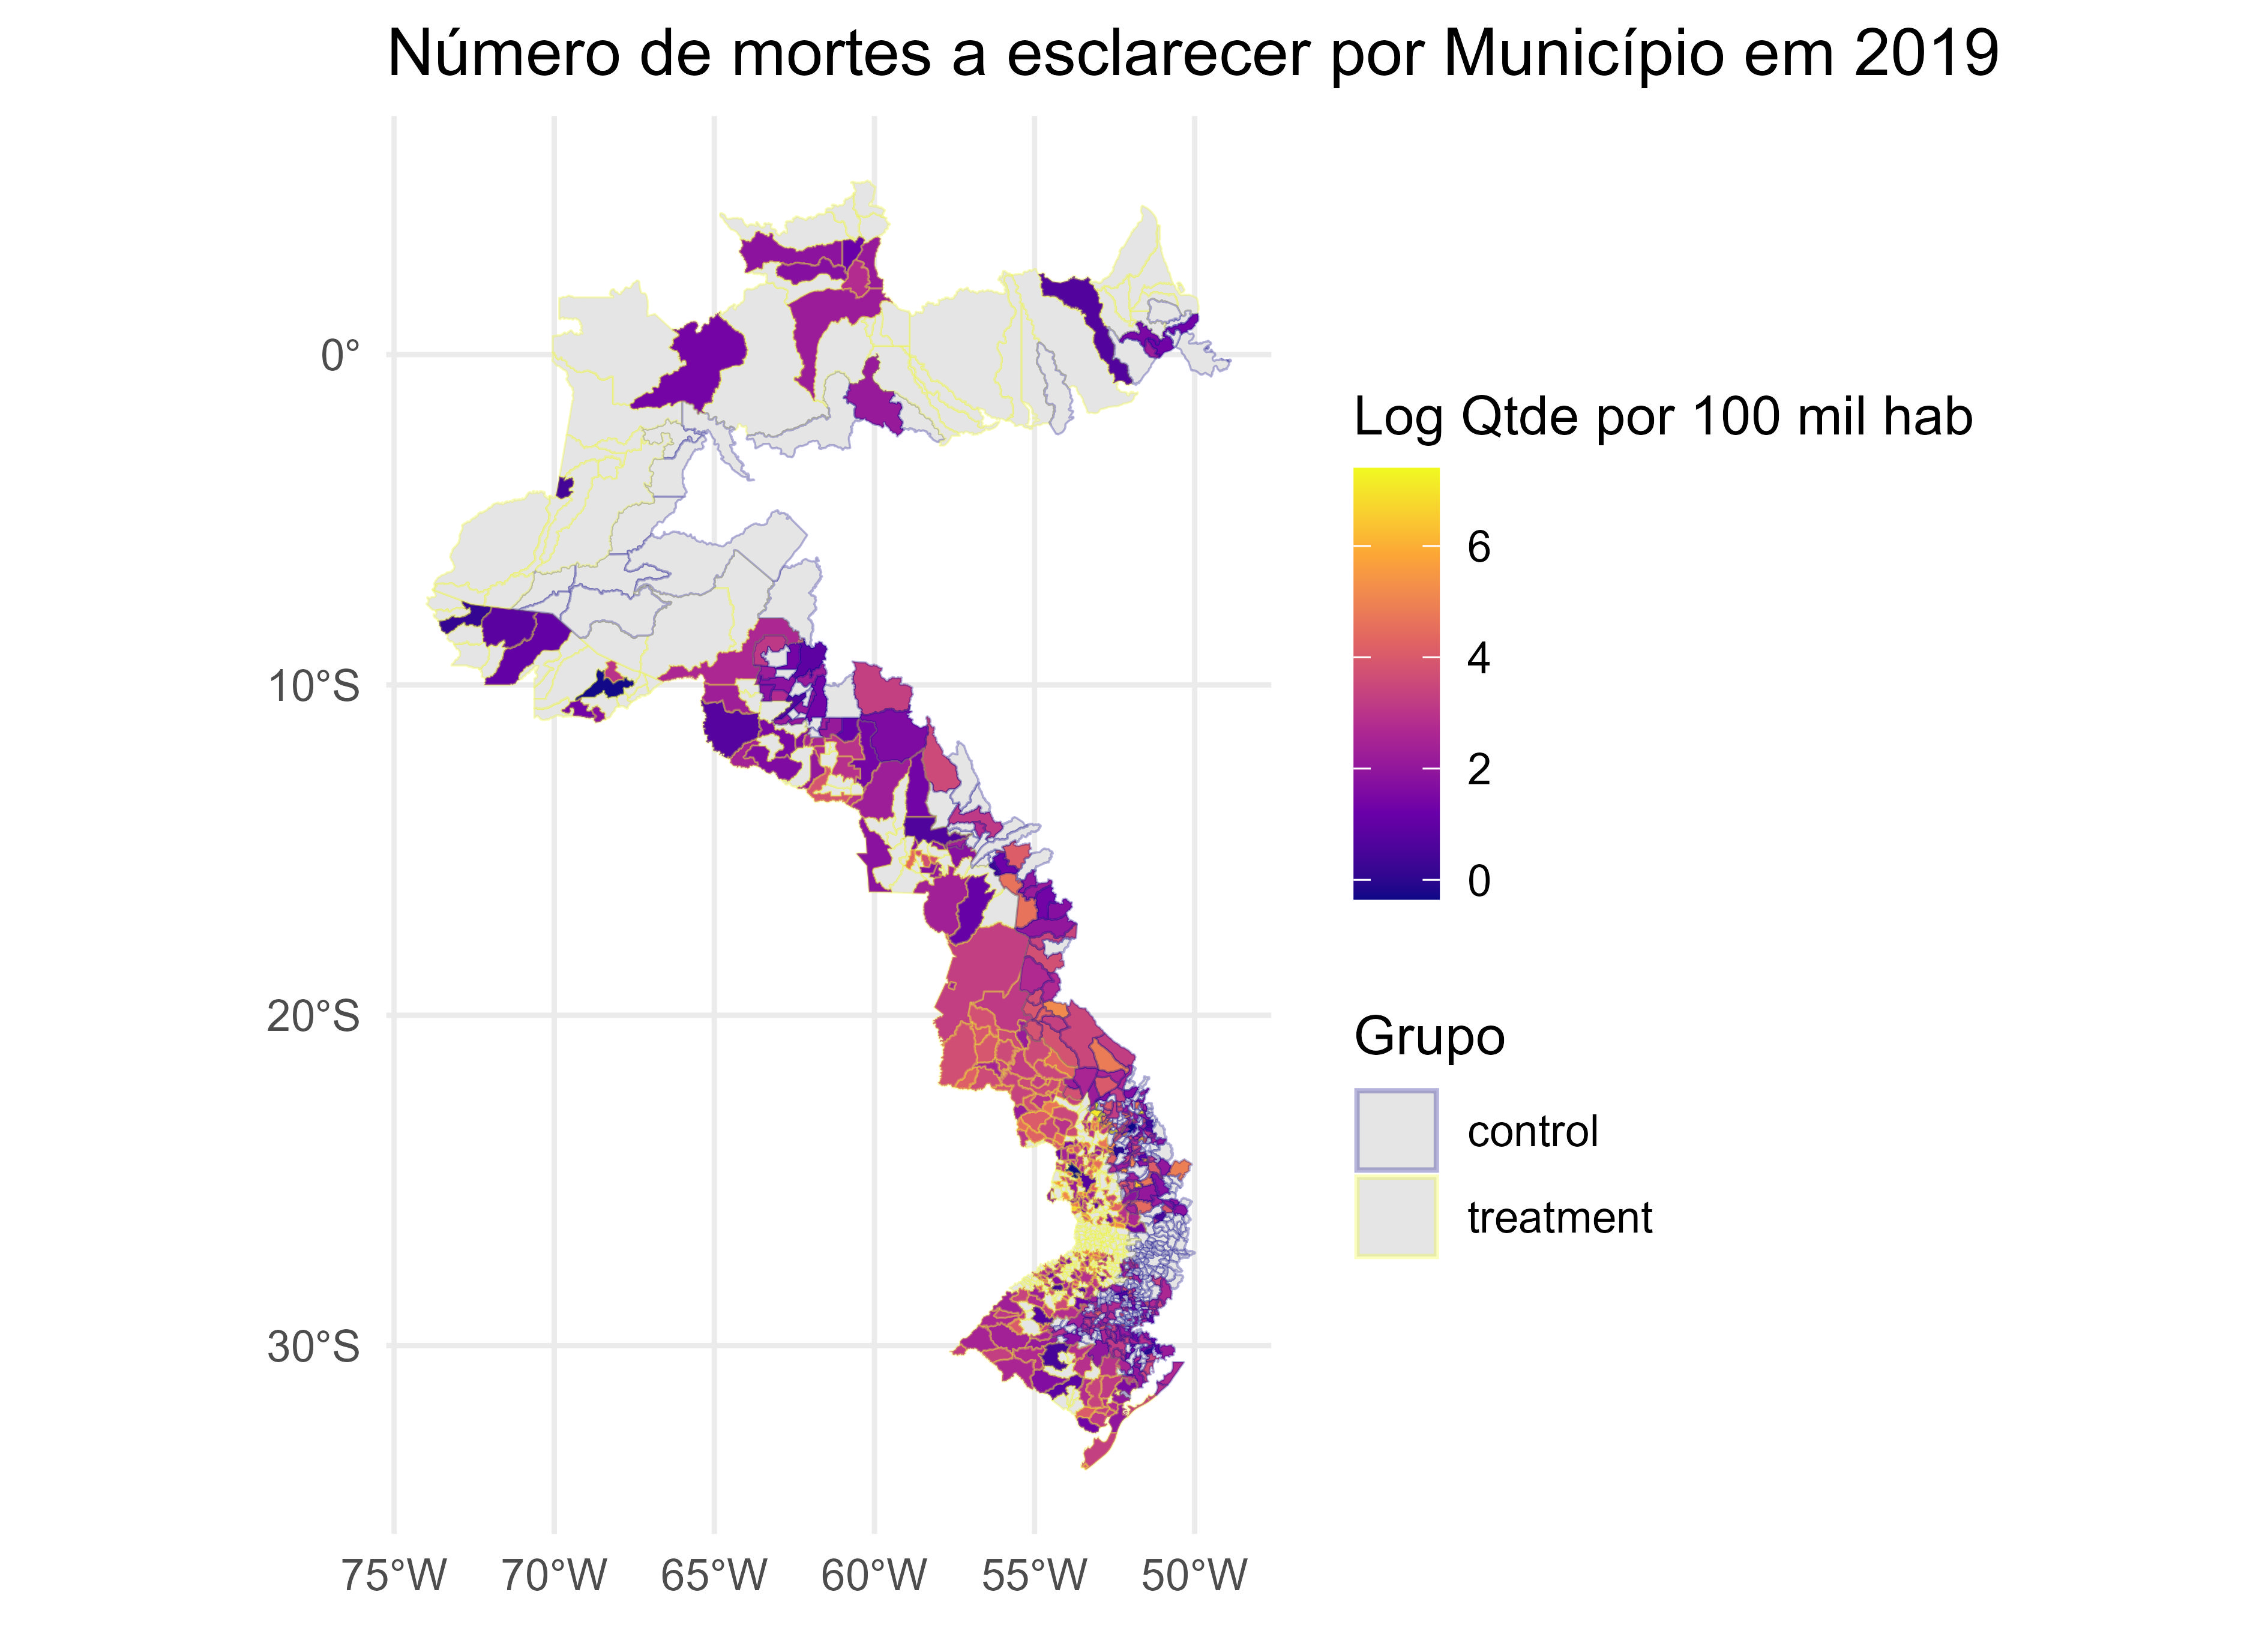
\includegraphics[width=1\linewidth]{figures/mapa_esclarecer}
		\label{fig:histoghom}
	\end{figure}
\end{frame}

\begin{frame}
	\begin{figure}
		\centering
		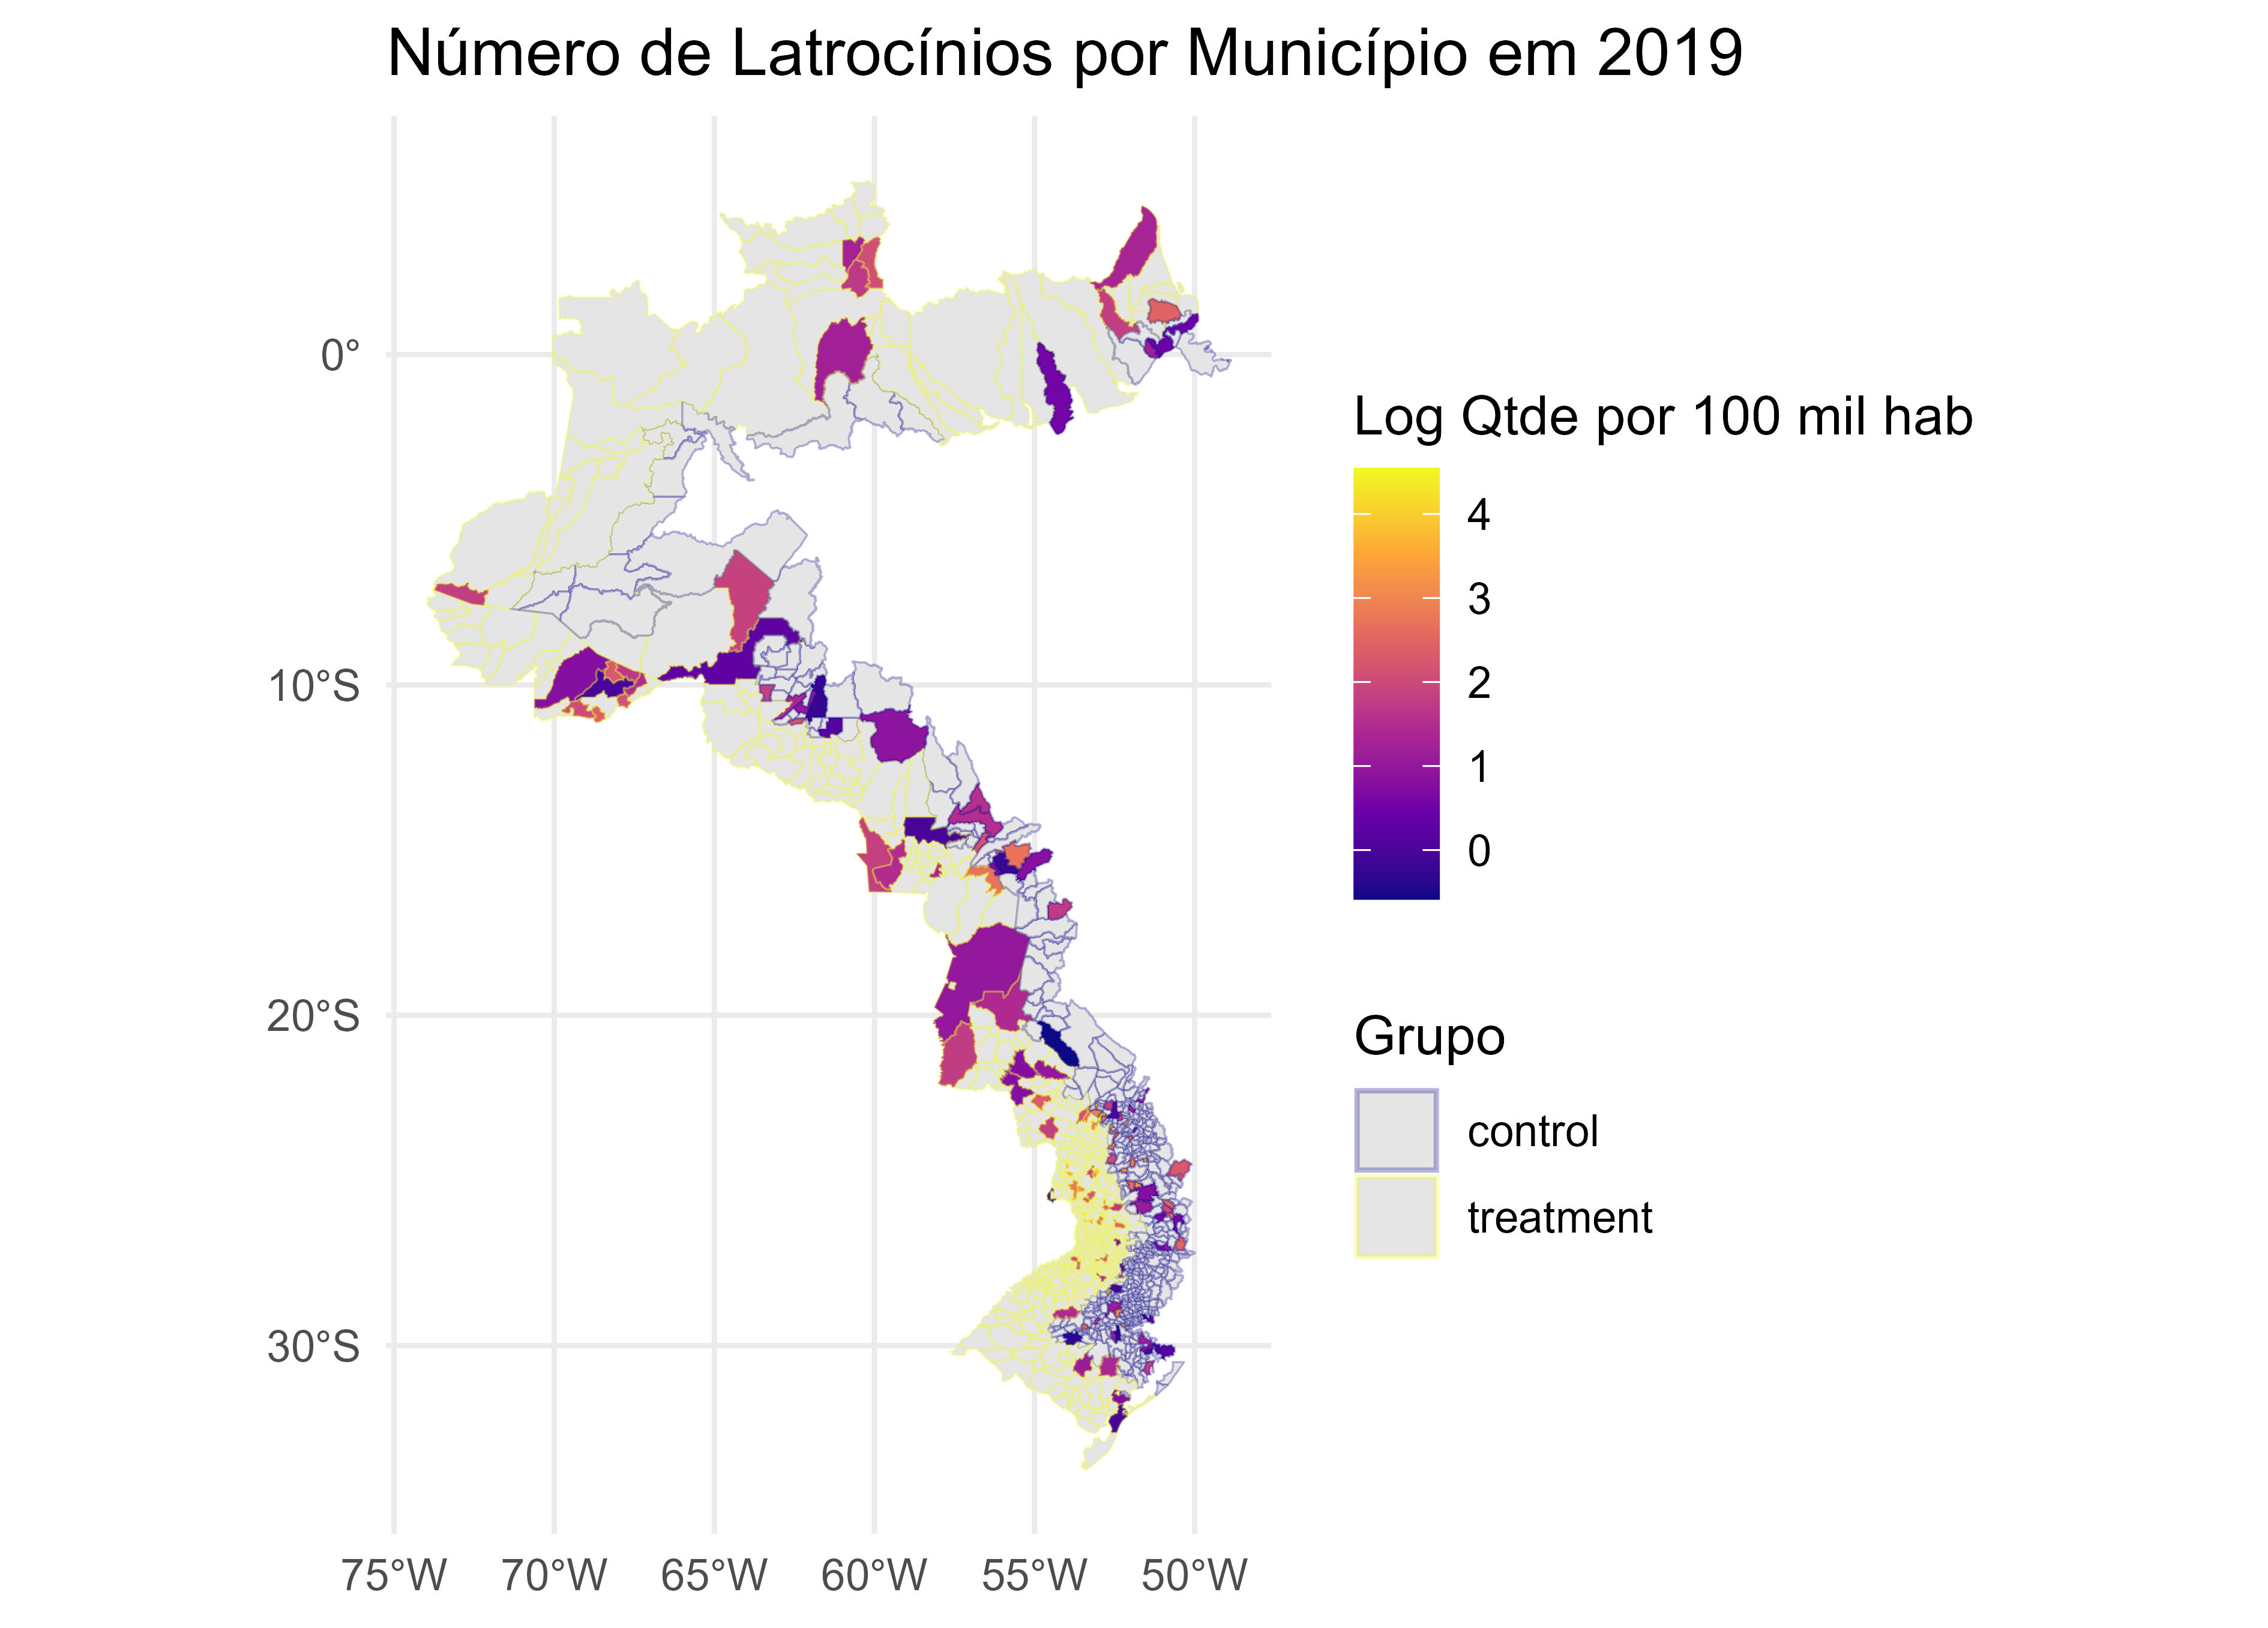
\includegraphics[width=1\linewidth]{figures/mapa_latrocinios}
		\label{fig:histoghom}
	\end{figure}
\end{frame}

\begin{frame}
	\begin{figure}
		\centering
		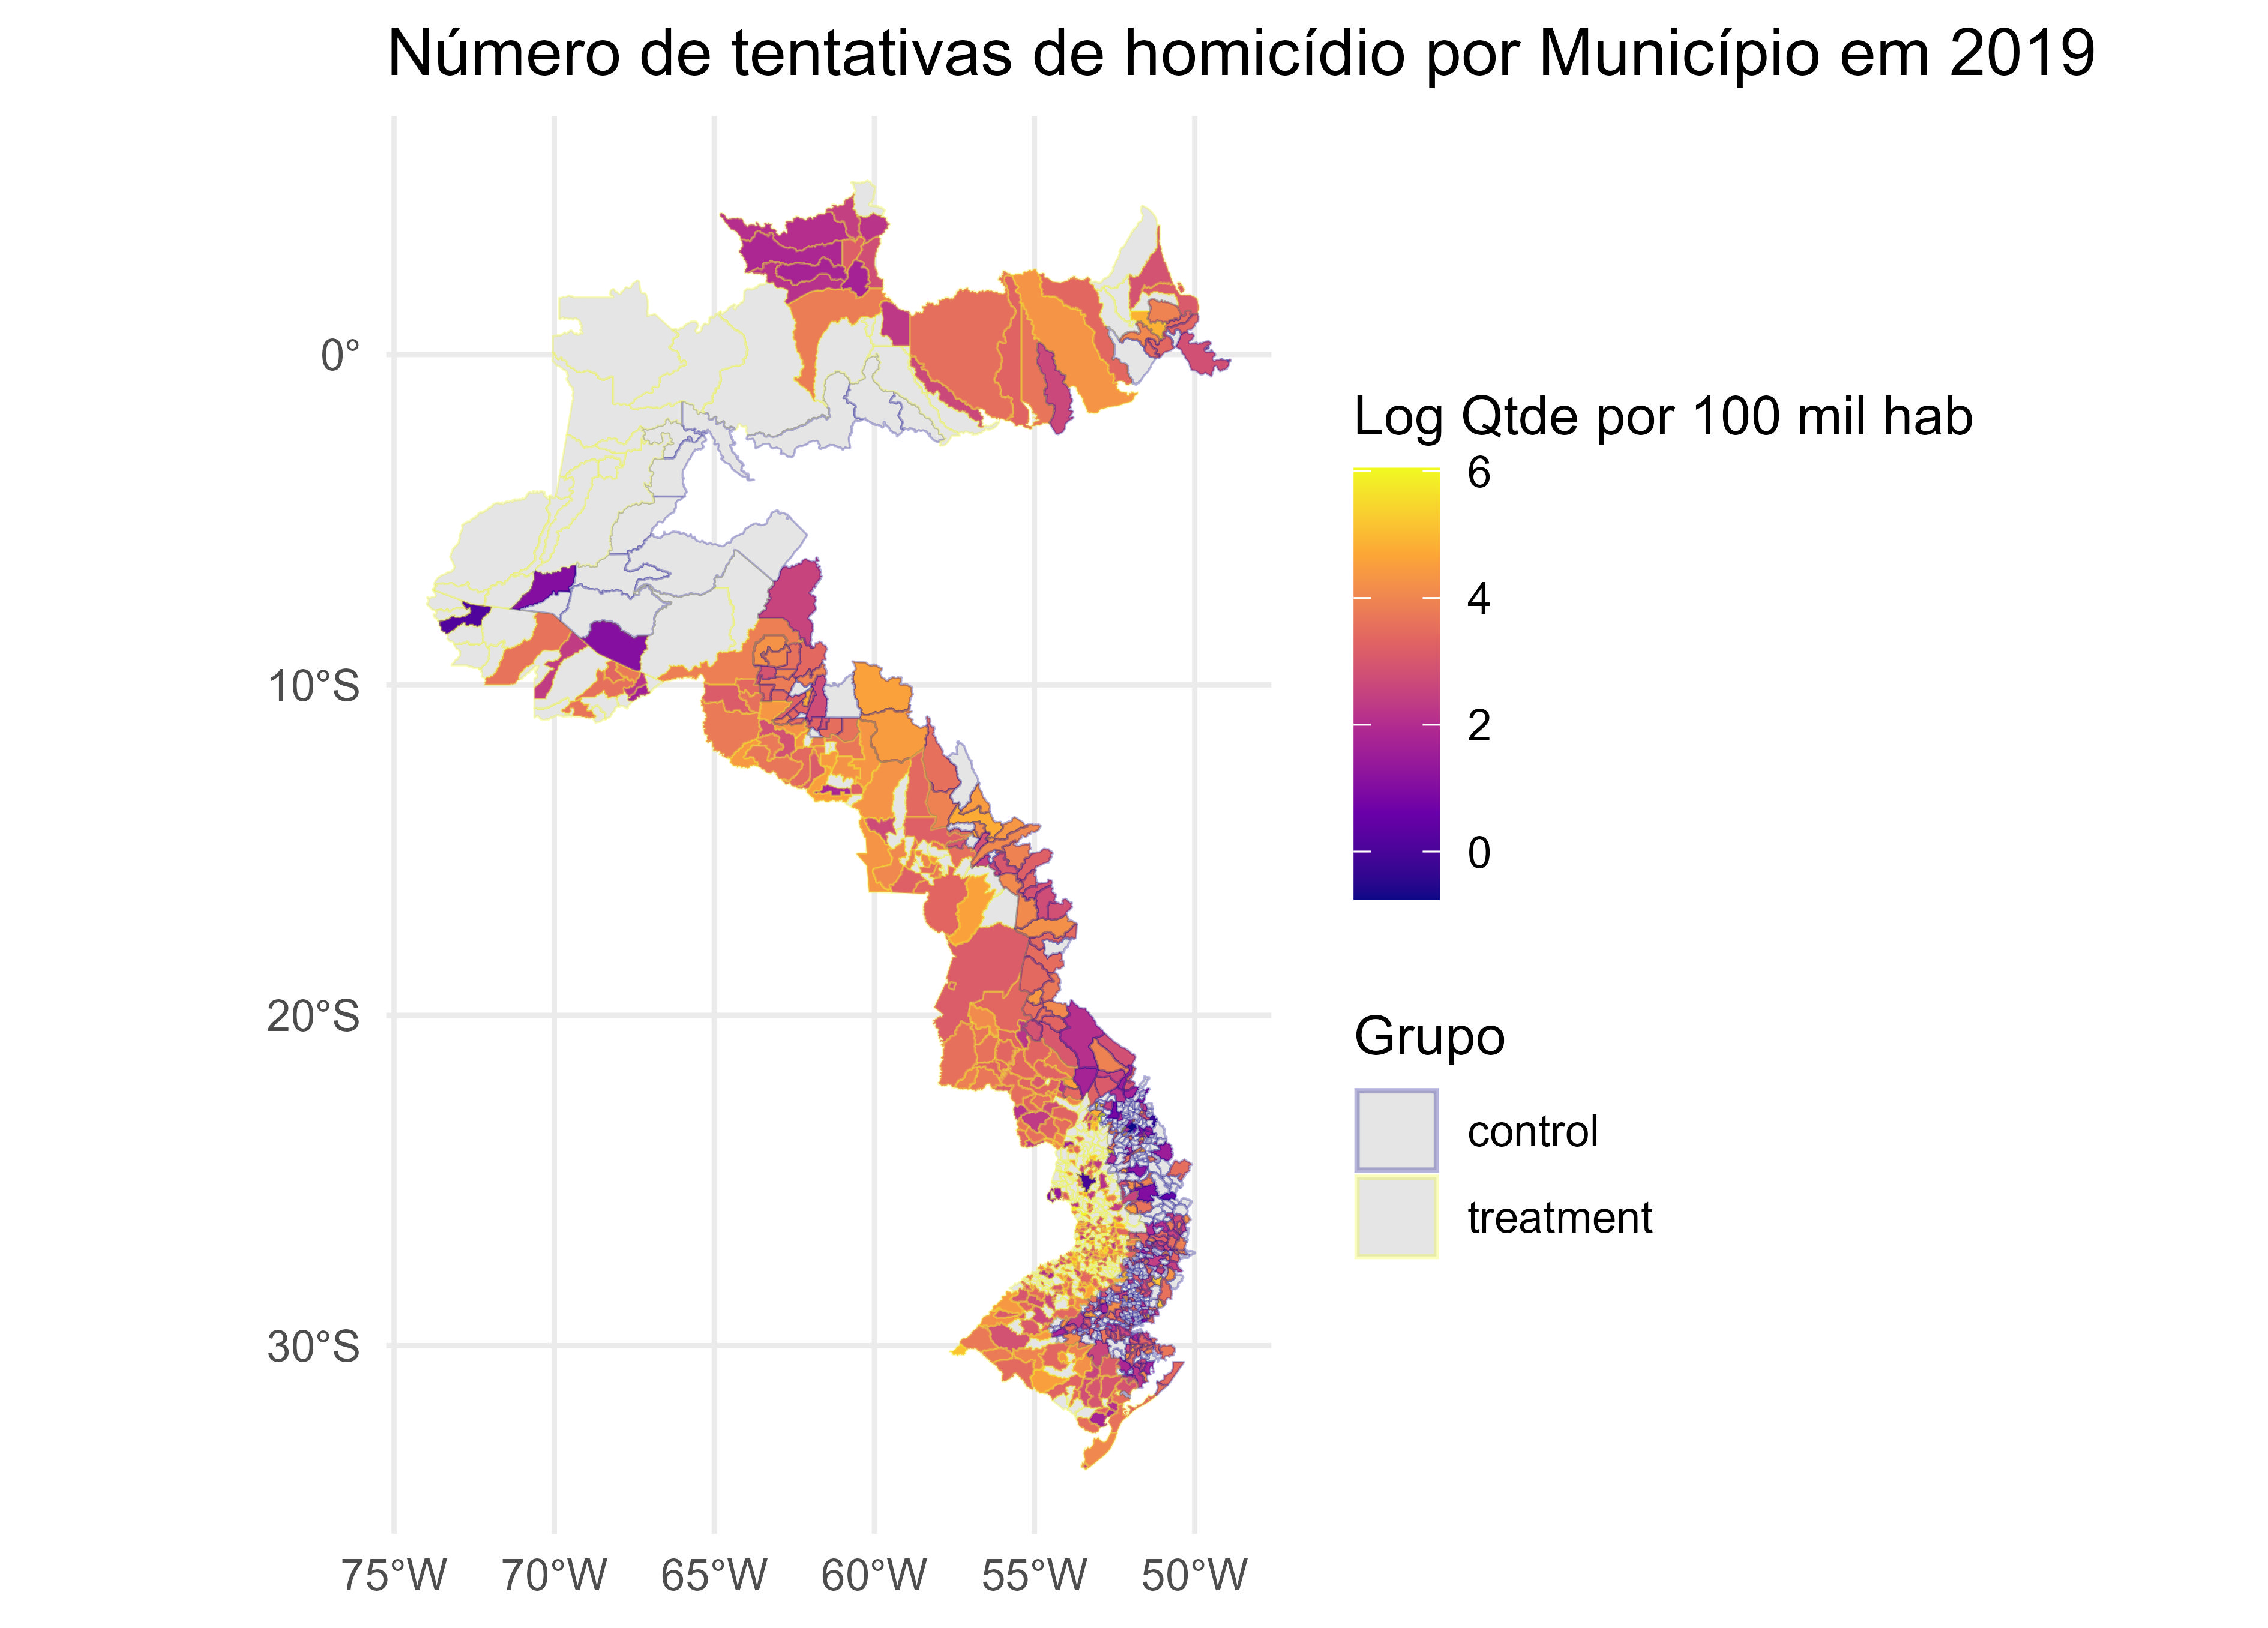
\includegraphics[width=1\linewidth]{figures/mapa_tentativas}
		\label{fig:histoghom}
	\end{figure}
\end{frame}

\begin{frame}{Homicídios}
	\begin{table}
	\tiny
\centering
\begin{talltblr}[         %% tabularray outer open
entry=none,label=none,
note{}={+ p < 0.1, * p < 0.05, ** p < 0.01, *** p < 0.001},
]                     %% tabularray outer close
{                     %% tabularray inner open
colspec={Q[]Q[]Q[]Q[]Q[]Q[]},
column{1}={halign=l,},
column{2}={halign=c,},
column{3}={halign=c,},
column{4}={halign=c,},
column{5}={halign=c,},
column{6}={halign=c,},
hline{6}={1,2,3,4,5,6}{solid, 0.05em, black},
}                     %% tabularray inner close
\toprule
& logit hom 2010 & ln hom 2011 & ln hom 2012 & ln hom 2013 & ln hom 2014 \\ \midrule %% TinyTableHeader
(Intercept) & \num{0.422}*** & \num{24.703}*** & \num{24.867}*** & \num{25.000}*** & \num{25.130}*** \\
& (\num{0.088})  & (\num{0.923})   & (\num{1.031})   & (\num{1.075})   & (\num{0.976})   \\
treatedTRUE & \num{0.158}    & \num{-1.213}    & \num{2.528}+    & \num{1.017}     & \num{1.547}     \\
& (\num{0.123})  & (\num{1.278})   & (\num{1.409})   & (\num{1.474})   & (\num{1.348})   \\
Num.Obs.    & \num{1131}     & \num{662}       & \num{694}       & \num{705}       & \num{717}       \\
R2          &                 & \num{0.001}     & \num{0.005}     & \num{0.001}     & \num{0.002}     \\
R2 Adj.     &                 & \num{0.000}     & \num{0.003}     & \num{-0.001}    & \num{0.000}     \\
AIC         & \num{1500.7}   & \num{5588.8}    & \num{6024.0}    & \num{6195.0}    & \num{6186.0}    \\
BIC         & \num{1510.8}   & \num{5602.3}    & \num{6037.6}    & \num{6208.6}    & \num{6199.8}    \\
Log.Lik.    &                 & \num{-2791.405} & \num{-3009.009} & \num{-3094.483} & \num{-3090.014} \\
F           & \num{1.654}    & \num{0.901}     & \num{3.220}     & \num{0.476}     & \num{1.317}     \\
RMSE        & \num{0.48}     & \num{16.41}     & \num{18.48}     & \num{19.50}     & \num{18.01}     \\
\bottomrule
\end{talltblr}
\end{table}

\end{frame}

\begin{frame}{Homicídios}
	\begin{table}
	\tiny
\centering
\begin{talltblr}[         %% tabularray outer open
entry=none,label=none,
note{}={+ p < 0.1, * p < 0.05, ** p < 0.01, *** p < 0.001},
]                     %% tabularray outer close
{                     %% tabularray inner open
colspec={Q[]Q[]Q[]Q[]Q[]Q[]},
column{1}={halign=l,},
column{2}={halign=c,},
column{3}={halign=c,},
column{4}={halign=c,},
column{5}={halign=c,},
column{6}={halign=c,},
hline{6}={1,2,3,4,5,6}{solid, 0.05em, black},
}                     %% tabularray inner close
\toprule
& ln hom 2015 & ln hom 2016 & ln hom 2017 & ln hom 2018 & ln hom 2019 \\ \midrule %% TinyTableHeader
(Intercept) & \num{3.029}*** & \num{3.076}*** & \num{3.094}*** & \num{2.969}*** & \num{2.972}*** \\
& (\num{0.037})  & (\num{0.039})  & (\num{0.037})  & (\num{0.039})  & (\num{0.038})  \\
treatedTRUE & \num{0.018}    & \num{0.060}    & \num{0.118}*   & \num{0.069}    & \num{0.032}    \\
& (\num{0.052})  & (\num{0.054})  & (\num{0.051})  & (\num{0.053})  & (\num{0.052})  \\
Num.Obs.    & \num{713}      & \num{728}      & \num{749}      & \num{737}      & \num{700}      \\
R2          & \num{0.000}    & \num{0.002}    & \num{0.007}    & \num{0.002}    & \num{0.001}    \\
R2 Adj.     & \num{-0.001}   & \num{0.000}    & \num{0.006}    & \num{0.001}    & \num{-0.001}   \\
AIC         & \num{1501.5}   & \num{1597.3}   & \num{1586.5}   & \num{1616.8}   & \num{1476.2}   \\
BIC         & \num{1515.3}   & \num{1611.1}   & \num{1600.4}   & \num{1630.6}   & \num{1489.9}   \\
Log.Lik.    & \num{-747.772} & \num{-795.667} & \num{-790.257} & \num{-805.398} & \num{-735.105} \\
F           & \num{0.127}    & \num{1.241}    & \num{5.351}    & \num{1.692}    & \num{0.362}    \\
RMSE        & \num{0.69}     & \num{0.72}     & \num{0.69}     & \num{0.72}     & \num{0.69}     \\
\bottomrule
\end{talltblr}
\end{table}

\end{frame}

\begin{frame}{Homicídios x estados}
	\begin{table}
	\tiny
\centering
\begin{adjustbox}{width=0.5\textwidth,center}
\begin{talltblr}[         %% tabularray outer open
entry=none,label=none,
note{}={+ p < 0.1, * p < 0.05, ** p < 0.01, *** p < 0.001},
]                     %% tabularray outer close
{                     %% tabularray inner open
colspec={Q[]Q[]Q[]Q[]Q[]Q[]},
column{1}={halign=l,},
column{2}={halign=c,},
column{3}={halign=c,},
column{4}={halign=c,},
column{5}={halign=c,},
column{6}={halign=c,},
hline{28}={1,2,3,4,5,6}{solid, 0.05em, black},
}                     %% tabularray inner close
\toprule
& ln hom 2010 & ln hom 2011 & ln hom 2012 & ln hom 2013 & ln hom 2014 \\ \midrule %% TinyTableHeader
(Intercept)      & \num{2.685}*** & \num{3.009}*** & \num{2.839}*** & \num{3.085}*** & \num{2.808}*** \\
& (\num{0.178})  & (\num{0.164})  & (\num{0.162})  & (\num{0.158})  & (\num{0.160})  \\
treatedTRUE      & \num{0.067}    & \num{-0.020}   & \num{0.133}*   & \num{0.033}    & \num{0.062}    \\
& (\num{0.053})  & (\num{0.053})  & (\num{0.054})  & (\num{0.052})  & (\num{0.052})  \\
abbrev\_stateAM & \num{-0.213}   & \num{-0.457}*  & \num{-0.298}   & \num{-0.393}+  & \num{-0.286}   \\
& (\num{0.224})  & (\num{0.205})  & (\num{0.208})  & (\num{0.203})  & (\num{0.204})  \\
abbrev\_stateAP & \num{0.548}*   & \num{0.131}    & \num{0.406}+   & \num{0.167}    & \num{0.575}*   \\
& (\num{0.260})  & (\num{0.236})  & (\num{0.239})  & (\num{0.245})  & (\num{0.242})  \\
abbrev\_stateMS & \num{0.368}+   & \num{0.171}    & \num{0.324}+   & \num{-0.016}   & \num{0.247}    \\
& (\num{0.192})  & (\num{0.181})  & (\num{0.178})  & (\num{0.173})  & (\num{0.176})  \\
abbrev\_stateMT & \num{0.563}**  & \num{0.244}    & \num{0.369}*   & \num{0.268}    & \num{0.650}*** \\
& (\num{0.198})  & (\num{0.186})  & (\num{0.186})  & (\num{0.182})  & (\num{0.182})  \\
abbrev\_statePA & \num{-0.492}   & \num{-0.621}+  & \num{0.205}    & \num{-0.525}   & \num{-0.303}   \\
& (\num{0.347})  & (\num{0.364})  & (\num{0.374})  & (\num{0.333})  & (\num{0.315})  \\
abbrev\_statePR & \num{0.442}*   & \num{0.184}    & \num{0.320}*   & \num{-0.016}   & \num{0.238}    \\
& (\num{0.178})  & (\num{0.165})  & (\num{0.162})  & (\num{0.158})  & (\num{0.160})  \\
abbrev\_stateRO & \num{0.554}**  & \num{0.050}    & \num{0.201}    & \num{-0.039}   & \num{0.524}**  \\
& (\num{0.200})  & (\num{0.187})  & (\num{0.186})  & (\num{0.180})  & (\num{0.183})  \\
abbrev\_stateRR & \num{0.336}    & \num{-0.025}   & \num{0.312}    & \num{0.270}    & \num{0.575}*   \\
& (\num{0.248})  & (\num{0.235})  & (\num{0.243})  & (\num{0.232})  & (\num{0.241})  \\
abbrev\_stateRS & \num{0.103}    & \num{-0.241}   & \num{-0.099}   & \num{-0.147}   & \num{0.083}    \\
& (\num{0.178})  & (\num{0.166})  & (\num{0.163})  & (\num{0.159})  & (\num{0.161})  \\
abbrev\_stateSC & \num{-0.075}   & \num{-0.454}*  & \num{-0.214}   & \num{-0.490}** & \num{-0.112}   \\
& (\num{0.187})  & (\num{0.177})  & (\num{0.176})  & (\num{0.170})  & (\num{0.171})  \\
abbrev\_stateSP & \num{-0.034}   & \num{-0.579}   & \num{-0.023}   & \num{-0.609}   & \num{-0.326}   \\
& (\num{0.351})  & (\num{0.368})  & (\num{0.345})  & (\num{0.416})  & (\num{0.374})  \\
Num.Obs.         & \num{705}      & \num{662}      & \num{694}      & \num{705}      & \num{717}      \\
R2               & \num{0.112}    & \num{0.129}    & \num{0.110}    & \num{0.078}    & \num{0.108}    \\
R2 Adj.          & \num{0.097}    & \num{0.113}    & \num{0.094}    & \num{0.062}    & \num{0.093}    \\
AIC              & \num{1466.7}   & \num{1340.4}   & \num{1454.2}   & \num{1442.4}   & \num{1487.1}   \\
BIC              & \num{1530.6}   & \num{1403.4}   & \num{1517.8}   & \num{1506.2}   & \num{1551.1}   \\
Log.Lik.         & \num{-719.373} & \num{-656.222} & \num{-713.108} & \num{-707.187} & \num{-729.532} \\
F                & \num{7.278}    & \num{8.044}    & \num{6.996}    & \num{4.909}    & \num{7.091}    \\
RMSE             & \num{0.67}     & \num{0.65}     & \num{0.68}     & \num{0.66}     & \num{0.67}     \\
\bottomrule
\end{adjustbox}
\end{talltblr}
\end{table}

\end{frame}

\begin{frame}{Homicídios x estados}
	\begin{table}
	\tiny
\centering
\begin{adjustbox}{width=0.5\textwidth,center}
\begin{talltblr}[         %% tabularray outer open
entry=none,label=none,
note{}={+ p < 0.1, * p < 0.05, ** p < 0.01, *** p < 0.001},
]                     %% tabularray outer close
{                     %% tabularray inner open
colspec={Q[]Q[]Q[]Q[]Q[]Q[]},
column{1}={halign=l,},
column{2}={halign=c,},
column{3}={halign=c,},
column{4}={halign=c,},
column{5}={halign=c,},
column{6}={halign=c,},
hline{28}={1,2,3,4,5,6}{solid, 0.05em, black},
}                     %% tabularray inner close
\toprule
& ln hom 2015 & ln hom 2016 & ln hom 2017 & ln hom 2018 & ln hom 2019 \\ \midrule %% TinyTableHeader
(Intercept)      & \num{2.949}*** & \num{3.334}***  & \num{3.568}***  & \num{3.444}***  & \num{3.228}***  \\
& (\num{0.155})  & (\num{0.163})   & (\num{0.154})   & (\num{0.170})   & (\num{0.159})   \\
treatedTRUE      & \num{0.002}    & \num{0.043}     & \num{0.089}+    & \num{0.019}     & \num{-0.007}    \\
& (\num{0.052})  & (\num{0.053})   & (\num{0.051})   & (\num{0.052})   & (\num{0.053})   \\
abbrev\_stateAM & \num{-0.386}+  & \num{-0.641}**  & \num{-0.719}*** & \num{-0.486}*   & \num{-0.160}    \\
& (\num{0.198})  & (\num{0.206})   & (\num{0.196})   & (\num{0.210})   & (\num{0.199})   \\
abbrev\_stateAP & \num{0.427}+   & \num{0.045}     & \num{-0.139}    & \num{-0.264}    & \num{0.090}     \\
& (\num{0.233})  & (\num{0.247})   & (\num{0.237})   & (\num{0.241})   & (\num{0.235})   \\
abbrev\_stateMS & \num{0.109}    & \num{-0.162}    & \num{-0.377}*   & \num{-0.399}*   & \num{-0.281}    \\
& (\num{0.173})  & (\num{0.180})   & (\num{0.171})   & (\num{0.187})   & (\num{0.177})   \\
abbrev\_stateMT & \num{0.462}*   & \num{0.066}     & \num{-0.164}    & \num{-0.115}    & \num{0.112}     \\
& (\num{0.180})  & (\num{0.190})   & (\num{0.177})   & (\num{0.192})   & (\num{0.184})   \\
abbrev\_statePA & \num{-0.104}   & \num{-0.769}*   & \num{-0.809}**  & \num{-1.226}*** & \num{-0.149}    \\
& (\num{0.335})  & (\num{0.321})   & (\num{0.310})   & (\num{0.306})   & (\num{0.312})   \\
abbrev\_statePR & \num{0.144}    & \num{-0.155}    & \num{-0.450}**  & \num{-0.432}*   & \num{-0.253}    \\
& (\num{0.156})  & (\num{0.163})   & (\num{0.155})   & (\num{0.171})   & (\num{0.160})   \\
abbrev\_stateRO & \num{0.315}+   & \num{0.011}     & \num{-0.305}+   & \num{-0.432}*   & \num{-0.163}    \\
& (\num{0.180})  & (\num{0.186})   & (\num{0.177})   & (\num{0.194})   & (\num{0.183})   \\
abbrev\_stateRR & \num{0.442}+   & \num{0.104}     & \num{-0.224}    & \num{0.430}+    & \num{0.328}     \\
& (\num{0.232})  & (\num{0.240})   & (\num{0.231})   & (\num{0.240})   & (\num{0.234})   \\
abbrev\_stateRS & \num{0.014}    & \num{-0.302}+   & \num{-0.440}**  & \num{-0.459}**  & \num{-0.240}    \\
& (\num{0.157})  & (\num{0.164})   & (\num{0.155})   & (\num{0.171})   & (\num{0.160})   \\
abbrev\_stateSC & \num{-0.126}   & \num{-0.745}*** & \num{-0.913}*** & \num{-0.910}*** & \num{-0.644}*** \\
& (\num{0.168})  & (\num{0.175})   & (\num{0.165})   & (\num{0.181})   & (\num{0.171})   \\
abbrev\_stateSP & \num{-0.569}   & \num{-0.882}*   & \num{-1.003}**  & \num{-1.060}**  & \num{-0.565}+   \\
& (\num{0.370})  & (\num{0.381})   & (\num{0.336})   & (\num{0.383})   & (\num{0.317})   \\
Num.Obs.         & \num{713}      & \num{728}       & \num{749}       & \num{737}       & \num{700}       \\
R2               & \num{0.073}    & \num{0.108}     & \num{0.098}     & \num{0.113}     & \num{0.076}     \\
R2 Adj.          & \num{0.057}    & \num{0.093}     & \num{0.083}     & \num{0.098}     & \num{0.060}     \\
AIC              & \num{1469.6}   & \num{1537.7}    & \num{1536.5}    & \num{1552.0}    & \num{1442.9}    \\
BIC              & \num{1533.5}   & \num{1602.0}    & \num{1601.1}    & \num{1616.4}    & \num{1506.6}    \\
Log.Lik.         & \num{-720.776} & \num{-754.847}  & \num{-754.235}  & \num{-761.999}  & \num{-707.461}  \\
F                & \num{4.600}    & \num{7.185}     & \num{6.676}     & \num{7.697}     & \num{4.737}     \\
RMSE             & \num{0.66}     & \num{0.68}      & \num{0.66}      & \num{0.68}      & \num{0.66}      \\
\bottomrule
\end{adjustbox}
\end{talltblr}
\end{table}

\end{frame}

\begin{frame}{Outros crimes}
	\begin{table}
	\tiny
\centering
\begin{talltblr}[         %% tabularray outer open
entry=none,label=none,
note{}={+ p < 0.1, * p < 0.05, ** p < 0.01, *** p < 0.001},
]                     %% tabularray outer close
{                     %% tabularray inner open
colspec={Q[]Q[]Q[]Q[]Q[]},
column{1}={halign=l,},
column{2}={halign=c,},
column{3}={halign=c,},
column{4}={halign=c,},
column{5}={halign=c,},
hline{6}={1,2,3,4,5}{solid, 0.05em, black},
}                     %% tabularray inner close
\toprule
& ln feminicidio & ln hom doloso & ln lesao & ln mandado \\ \midrule %% TinyTableHeader
(Intercept) & \num{1.797}*** & \num{3.173}*** & \num{1.736}*** & \num{4.636}*** \\
& (\num{0.144})  & (\num{0.062})  & (\num{0.237})  & (\num{0.068})  \\
treatedTRUE & \num{-0.398}*  & \num{-0.180}*  & \num{-0.026}   & \num{-0.052}   \\
& (\num{0.194})  & (\num{0.085})  & (\num{0.355})  & (\num{0.091})  \\
Num.Obs.    & \num{155}      & \num{623}      & \num{72}       & \num{626}      \\
R2          & \num{0.027}    & \num{0.007}    & \num{0.000}    & \num{0.001}    \\
R2 Adj.     & \num{0.020}    & \num{0.006}    & \num{-0.014}   & \num{-0.001}   \\
AIC         & \num{990.6}    & \num{5682.8}   & \num{514.8}    & \num{7711.0}   \\
BIC         & \num{999.7}    & \num{5696.1}   & \num{521.6}    & \num{7724.4}   \\
Log.Lik.    & \num{-247.646} & \num{-920.847} & \num{-130.240} & \num{-967.972} \\
F           & \num{4.201}    & \num{4.462}    & \num{0.005}    & \num{0.327}    \\
RMSE        & \num{1.20}     & \num{1.06}     & \num{1.48}     & \num{1.14}     \\
\bottomrule
\end{talltblr}
\end{table}

\end{frame}

\begin{frame}{Outros crimes}
	\begin{table}
	\tiny
\centering
\begin{talltblr}[         %% tabularray outer open
entry=none,label=none,
note{}={+ p < 0.1, * p < 0.05, ** p < 0.01, *** p < 0.001},
]                     %% tabularray outer close
{                     %% tabularray inner open
colspec={Q[]Q[]Q[]Q[]Q[]},
column{1}={halign=l,},
column{2}={halign=c,},
column{3}={halign=c,},
column{4}={halign=c,},
column{5}={halign=c,},
hline{6}={1,2,3,4,5}{solid, 0.05em, black},
}                     %% tabularray inner close
\toprule
& ln transito & ln esclarecer & ln latrocinio & ln tentativa \\ \midrule %% TinyTableHeader
(Intercept) & \num{3.091}*** & \num{3.120}*** & \num{1.816}*** & \num{3.339}*** \\
& (\num{0.061})  & (\num{0.078})  & (\num{0.141})  & (\num{0.058})  \\
treatedTRUE & \num{-0.234}** & \num{-0.249}*  & \num{-0.046}   & \num{-0.012}   \\
& (\num{0.086})  & (\num{0.110})  & (\num{0.213})  & (\num{0.080})  \\
Num.Obs.    & \num{587}      & \num{532}      & \num{136}      & \num{571}      \\
R2          & \num{0.013}    & \num{0.010}    & \num{0.000}    & \num{0.000}    \\
R2 Adj.     & \num{0.011}    & \num{0.008}    & \num{-0.007}   & \num{-0.002}   \\
AIC         & \num{5208.2}   & \num{4948.2}   & \num{934.9}    & \num{5374.2}   \\
BIC         & \num{5221.3}   & \num{4961.0}   & \num{943.6}    & \num{5387.2}   \\
Log.Lik.    & \num{-855.702} & \num{-878.376} & \num{-220.270} & \num{-781.120} \\
F           & \num{7.437}    & \num{5.153}    & \num{0.047}    & \num{0.023}    \\
RMSE        & \num{1.04}     & \num{1.26}     & \num{1.22}     & \num{0.95}     \\
\bottomrule
\end{talltblr}
\end{table}

\end{frame}

\begin{frame}{Outros crimes x estados}
	\begin{table}
	\tiny
\centering
\begin{adjustbox}{width=0.5\textwidth,center}
\begin{talltblr}[         %% tabularray outer open
entry=none,label=none,
note{}={+ p < 0.1, * p < 0.05, ** p < 0.01, *** p < 0.001},
]                     %% tabularray outer close
{                     %% tabularray inner open
colspec={Q[]Q[]Q[]Q[]Q[]},
column{1}={halign=l,},
column{2}={halign=c,},
column{3}={halign=c,},
column{4}={halign=c,},
column{5}={halign=c,},
hline{28}={1,2,3,4,5}{solid, 0.05em, black},
}                     %% tabularray inner close
\toprule
& ln feminicidio & ln hom doloso & ln lesao & ln mandado \\ \midrule %% TinyTableHeader
(Intercept)      & \num{1.398}**  & \num{3.273}*** & \num{1.252}    & \num{4.797}***  \\
& (\num{0.429})  & (\num{0.255})  & (\num{1.040})  & (\num{0.204})   \\
treatedTRUE      & \num{-0.205}   & \num{-0.156}+  & \num{0.276}    & \num{0.079}     \\
& (\num{0.192})  & (\num{0.085})  & (\num{0.359})  & (\num{0.073})   \\
abbrev\_stateAP & \num{-0.960}   & \num{0.037}    & \num{0.355}    & \num{-0.553}    \\
& (\num{0.760})  & (\num{0.366})  & (\num{1.226})  & (\num{0.337})   \\
abbrev\_stateMS & \num{-0.393}   & \num{-0.252}   & \num{0.198}    & \num{0.173}     \\
& (\num{0.472})  & (\num{0.282})  & (\num{1.134})  & (\num{0.221})   \\
abbrev\_stateMT & \num{-0.215}   & \num{0.041}    & \num{0.036}    & \num{-0.223}    \\
& (\num{0.502})  & (\num{0.294})  & (\num{1.209})  & (\num{0.250})   \\
abbrev\_statePA & \num{-0.161}   & \num{-0.407}   &                 & \num{-1.184}**  \\
& (\num{1.169})  & (\num{0.482})  &                 & (\num{0.404})   \\
abbrev\_statePR & \num{1.057}*   & \num{0.287}    & \num{1.206}    & \num{1.090}***  \\
& (\num{0.436})  & (\num{0.256})  & (\num{1.040})  & (\num{0.213})   \\
abbrev\_stateRO & \num{-0.856}   & \num{-0.193}   & \num{0.009}    & \num{-0.481}*   \\
& (\num{0.590})  & (\num{0.286})  & (\num{1.226})  & (\num{0.230})   \\
abbrev\_stateRR & \num{-0.066}   & \num{-0.045}   & \num{-0.039}   & \num{-1.931}*** \\
& (\num{0.736})  & (\num{0.364})  & (\num{1.381})  & (\num{0.362})   \\
abbrev\_stateRS & \num{0.182}    & \num{-0.319}   & \num{-0.685}   & \num{-0.949}*** \\
& (\num{0.421})  & (\num{0.256})  & (\num{1.050})  & (\num{0.204})   \\
abbrev\_stateSC & \num{0.817}    & \num{-0.556}*  & \num{-0.263}   & \num{-0.158}    \\
& (\num{0.513})  & (\num{0.283})  & (\num{1.381})  & (\num{0.208})   \\
abbrev\_stateAM &                 & \num{-1.007}*  & \num{-0.179}   & \num{-1.182}*** \\
&                 & (\num{0.393})  & (\num{1.393})  & (\num{0.251})   \\
abbrev\_stateSP &                 & \num{-1.077}*  &                 & \num{0.678}*    \\
&                 & (\num{0.489})  &                 & (\num{0.323})   \\
Num.Obs.         & \num{155}      & \num{623}      & \num{72}       & \num{626}       \\
R2               & \num{0.253}    & \num{0.100}    & \num{0.259}    & \num{0.425}     \\
R2 Adj.          & \num{0.201}    & \num{0.082}    & \num{0.138}    & \num{0.413}     \\
AIC              & \num{967.6}    & \num{5643.9}   & \num{511.1}    & \num{7387.5}    \\
BIC              & \num{1004.1}   & \num{5705.9}   & \num{538.5}    & \num{7449.6}    \\
Log.Lik.         & \num{-227.151} & \num{-890.379} & \num{-119.432} & \num{-795.195}  \\
F                & \num{4.874}    & \num{5.626}    & \num{2.137}    & \num{37.681}    \\
RMSE             & \num{1.05}     & \num{1.01}     & \num{1.27}     & \num{0.86}      \\
\bottomrule
\end{adjustbox}
\end{talltblr}
\end{table}

\end{frame}

\begin{frame}{Outros crimes x estados}
	\begin{table}
	\tiny
\centering
\begin{adjustbox}{width=0.4\textwidth,center}
\begin{talltblr}[         %% tabularray outer open
entry=none,label=none,
note{}={+ p < 0.1, * p < 0.05, ** p < 0.01, *** p < 0.001},
]                     %% tabularray outer close
{                     %% tabularray inner open
colspec={Q[]Q[]Q[]Q[]Q[]},
column{1}={halign=l,},
column{2}={halign=c,},
column{3}={halign=c,},
column{4}={halign=c,},
column{5}={halign=c,},
hline{28}={1,2,3,4,5}{solid, 0.05em, black},
}                     %% tabularray inner close
\toprule
& ln transito & ln esclarecer & ln latrocinio & ln tentativa \\ \midrule %% TinyTableHeader
(Intercept)      & \num{2.909}*** & \num{1.331}**  & \num{1.612}*** & \num{2.670}*** \\
& (\num{0.267})  & (\num{0.448})  & (\num{0.440})  & (\num{0.317})  \\
treatedTRUE      & \num{-0.155}+  & \num{-0.227}*  & \num{-0.018}   & \num{0.022}    \\
& (\num{0.087})  & (\num{0.103})  & (\num{0.215})  & (\num{0.080})  \\
abbrev\_stateAM & \num{-1.179}*  & \num{0.124}    & \num{0.230}    & \num{-1.126}+  \\
& (\num{0.567})  & (\num{0.797})  & (\num{0.858})  & (\num{0.616})  \\
abbrev\_stateAP & \num{-0.188}   & \num{0.159}    & \num{-0.164}   & \num{0.944}*   \\
& (\num{0.387})  & (\num{0.727})  & (\num{0.632})  & (\num{0.436})  \\
abbrev\_stateMS & \num{-0.144}   & \num{2.314}*** & \num{-0.459}   & \num{0.631}+   \\
& (\num{0.292})  & (\num{0.461})  & (\num{0.528})  & (\num{0.329})  \\
abbrev\_stateMT & \num{-0.077}   & \num{1.104}*   & \num{-0.231}   & \num{1.014}**  \\
& (\num{0.312})  & (\num{0.493})  & (\num{0.500})  & (\num{0.344})  \\
abbrev\_statePA & \num{-1.480}** &                 & \num{-1.068}   & \num{0.579}    \\
& (\num{0.564})  &                 & (\num{1.171})  & (\num{0.464})  \\
abbrev\_statePR & \num{0.493}+   & \num{2.246}*** & \num{1.022}*   & \num{0.566}+   \\
& (\num{0.270})  & (\num{0.448})  & (\num{0.434})  & (\num{0.323})  \\
abbrev\_stateRO & \num{-0.079}   & \num{0.872}+   & \num{-0.672}   & \num{0.980}**  \\
& (\num{0.308})  & (\num{0.484})  & (\num{0.591})  & (\num{0.339})  \\
abbrev\_stateRR & \num{-0.560}   & \num{0.873}    & \num{-0.035}   & \num{-0.314}   \\
& (\num{0.437})  & (\num{0.642})  & (\num{0.665})  & (\num{0.414})  \\
abbrev\_stateRS & \num{0.195}    & \num{1.592}*** & \num{-0.283}   & \num{0.692}*   \\
& (\num{0.266})  & (\num{0.447})  & (\num{0.455})  & (\num{0.316})  \\
abbrev\_stateSC & \num{-0.012}   &                 & \num{-0.528}   & \num{0.648}*   \\
& (\num{0.284})  &                 & (\num{0.642})  & (\num{0.326})  \\
abbrev\_stateSP & \num{-0.228}   & \num{0.991}    & \num{-0.322}   & \num{-0.500}   \\
& (\num{0.490})  & (\num{0.650})  & (\num{1.171})  & (\num{0.492})  \\
Num.Obs.         & \num{587}      & \num{532}      & \num{136}      & \num{571}      \\
R2               & \num{0.092}    & \num{0.188}    & \num{0.287}    & \num{0.084}    \\
R2 Adj.          & \num{0.073}    & \num{0.173}    & \num{0.218}    & \num{0.064}    \\
AIC              & \num{5181.1}   & \num{4860.2}   & \num{910.9}    & \num{5346.3}   \\
BIC              & \num{5242.3}   & \num{4911.6}   & \num{951.6}    & \num{5407.2}   \\
Log.Lik.         & \num{-831.140} & \num{-825.400} & \num{-197.266} & \num{-756.183} \\
F                & \num{4.836}    & \num{12.100}   & \num{4.131}    & \num{4.246}    \\
RMSE             & \num{1.00}     & \num{1.14}     & \num{1.03}     & \num{0.91}     \\
\bottomrule
\end{talltblr}
\end{adjustbox}
\end{table}

\end{frame}

\begin{frame}{Efeitos marginais no modelo Logit: homicídios em 2019}
	\begin{tiny}
		logitmfx(formula = `valor-2019` ~ treated + abbrev state, data = df rdd3)
		
		Marginal Effects: \\
		dF/dx Std. Err.       z     P>|z|    \\
		treatedTRUE    -0.053197  0.030011 -1.7725   0.07630 . \\ 
		abbrev stateAM -0.172346  0.220765 -0.7807   0.43499    \\
		abbrev stateAP  0.052374  0.273576  0.1914   0.84818    \\
		abbrev stateMS -0.236153  0.194370 -1.2150   0.22438    \\
		abbrev stateMT -0.312723  0.180691 -1.7307   0.08350 .  \\
		abbrev statePA -0.139558  0.327589 -0.4260   0.67010    \\
		abbrev statePR -0.411885  0.160189 -2.5712   0.01013 *  \\
		abbrev stateRO -0.170666  0.207871 -0.8210   0.41164    \\
		abbrev stateRR  0.073823  0.262651  0.2811   0.77866    \\
		abbrev stateRS -0.539566  0.135978 -3.9680 7.246e-05 *** \\
		abbrev stateSC -0.522341  0.119584 -4.3680 1.254e-05 ***\\
		abbrev stateSP -0.517981  0.106387 -4.8689 1.122e-06 ***\\
		---
		Signif. codes:  0 ‘***’ 0.001 ‘**’ 0.01 ‘*’ 0.05 ‘.’ 0.1 ‘ ’ 1\\
		
		dF/dx is for discrete change for the following variables:
		
		[1] "treatedTRUE"    "abbrev_stateAM" "abbrev_stateAP" "abbrev_stateMS"\\
		[5] "abbrev_stateMT" "abbrev_statePA" "abbrev_statePR" "abbrev_stateRO"\\
		[9] "abbrev_stateRR" "abbrev_stateRS" "abbrev_stateSC" "abbrev_stateSP"\\
	\end{tiny}
\end{frame}

\begin{frame}{Efeitos marginais no modelo Logit: feminicídio}
	\begin{tiny}
logitmfx(formula = feminicidio_pc ~ treated + abbrev_state, data = df_rdd3)

Marginal Effects:\\
dF/dx   Std. Err.       z  P>|z|\\
treatedTRUE     0.00077599  0.02016223  0.0385 0.9693\\
abbrev_stateAM -0.12173647  1.29786668 -0.0938 0.9253\\
abbrev_stateAP -0.04299474  0.88357972 -0.0487 0.9612\\
abbrev_stateMS -0.03394544  0.68790326 -0.0493 0.9606\\
abbrev_stateMT -0.03731372  0.75905669 -0.0492 0.9608\\
abbrev_statePA -0.05479633  1.14153841 -0.0480 0.9617\\
abbrev_statePR -0.07277392  1.45622032 -0.0500 0.9601\\
abbrev_stateRO -0.06334246  1.31853476 -0.0480 0.9617\\
abbrev_stateRR -0.04317265  0.88739169 -0.0487 0.9612\\
abbrev_stateRS -0.08877745  1.73758430 -0.0511 0.9593\\
abbrev_stateSC -0.08269575  1.70274814 -0.0486 0.9613\\
abbrev_stateSP -0.09301673  1.67232474 -0.0556 0.9556\\

dF/dx is for discrete change for the following variables:

[1] "treatedTRUE"    "abbrev_stateAM" "abbrev_stateAP" "abbrev_stateMS"\\
[5] "abbrev_stateMT" "abbrev_statePA" "abbrev_statePR" "abbrev_stateRO"\\
[9] "abbrev_stateRR" "abbrev_stateRS" "abbrev_stateSC" "abbrev_stateSP"\\
\end{tiny}
\end{frame}

\begin{frame}{Efeitos marginais no modelo Logit: homicídio doloso}
	\begin{tiny}
logitmfx(formula = hom_doloso_pc ~ treated + abbrev_state, data = df_rdd3)

Marginal Effects:\\
dF/dx Std. Err.       z     P>|z|    \\
treatedTRUE    -0.015842  0.031921 -0.4963 0.6196926    \\
abbrev_stateAM -0.446614  0.082314 -5.4257 5.772e-08 ***\\
abbrev_stateAP  0.231801  0.190925  1.2141 0.2247110    \\
abbrev_stateMS -0.095675  0.155587 -0.6149 0.5386033    \\
abbrev_stateMT -0.147840  0.154205 -0.9587 0.3377004    \\
abbrev_statePA  0.064543  0.282128  0.2288 0.8190471    \\
abbrev_statePR -0.239790  0.134895 -1.7776 0.0754685 .  \\
abbrev_stateRO  0.160652  0.147638  1.0882 0.2765272    \\
abbrev_stateRR  0.236599  0.187406  1.2625 0.2067728    \\
abbrev_stateRS -0.427372  0.115966 -3.6853 0.0002284 ***\\
abbrev_stateSC -0.461700  0.089885 -5.1366 2.798e-07 ***\\
abbrev_stateSP -0.354482  0.139175 -2.5470 0.0108648 *  \\
---
Signif. codes:  0 ‘***’ 0.001 ‘**’ 0.01 ‘*’ 0.05 ‘.’ 0.1 ‘ ’ 1

dF/dx is for discrete change for the following variables:\\

[1] "treatedTRUE"    "abbrev_stateAM" "abbrev_stateAP" "abbrev_stateMS"\\
[5] "abbrev_stateMT" "abbrev_statePA" "abbrev_statePR" "abbrev_stateRO"\\
[9] "abbrev_stateRR" "abbrev_stateRS" "abbrev_stateSC" "abbrev_stateSP"\\
\end{tiny}
\end{frame}

\begin{frame}{Efeitos marginais no modelo Logit: lesão}
	\begin{tiny}
logitmfx(formula = lesao_pc ~ treated + abbrev_state, data = df_rdd3)

Marginal Effects:\\
dF/dx  Std. Err.       z  P>|z|\\
treatedTRUE    -0.0175434  0.1484350 -0.1182 0.9059\\
abbrev_stateAM -0.0190945  0.1666577 -0.1146 0.9088\\
abbrev_stateAP  0.0732503  0.5790519  0.1265 0.8993\\
abbrev_stateMS -0.0058122  0.0585650 -0.0992 0.9209\\
abbrev_stateMT -0.0172280  0.1501973 -0.1147 0.9087\\
abbrev_statePA -0.0467362  0.3280809 -0.1425 0.8867\\
abbrev_statePR -0.0064639  0.0625423 -0.1034 0.9177\\
abbrev_stateRO -0.0138404  0.1217282 -0.1137 0.9095\\
abbrev_stateRR  0.0215073  0.1887734  0.1139 0.9093\\
abbrev_stateRS -0.0402723  0.3423881 -0.1176 0.9064\\
abbrev_stateSC -0.0488055  0.4236650 -0.1152 0.9083\\
abbrev_stateSP -0.0498048  0.2654572 -0.1876 0.8512\\

dF/dx is for discrete change for the following variables:

[1] "treatedTRUE"    "abbrev_stateAM" "abbrev_stateAP" "abbrev_stateMS"\\
[5] "abbrev_stateMT" "abbrev_statePA" "abbrev_statePR" "abbrev_stateRO"\\
[9] "abbrev_stateRR" "abbrev_stateRS" "abbrev_stateSC" "abbrev_stateSP"\\
\end{tiny}
\\\end{frame}

\begin{frame}{Efeitos marginais no modelo Logit: mandado}
	\begin{tiny}
logitmfx(formula = mandado_pc ~ treated + abbrev_state, data = df_rdd3)

Marginal Effects:\\
dF/dx   Std. Err.       z     P>|z|    \\
treatedTRUE     0.00060792  0.03202285  0.0190  0.984854    \\
abbrev_stateAM -0.18921777  0.30718852 -0.6160  0.537917    \\
abbrev_stateAP -0.49867070  0.47588907 -1.0479  0.294698    \\
abbrev_stateMS  0.00019357  0.27215860  0.0007  0.999433    \\
abbrev_stateMT -0.57540814  0.59238226 -0.9713  0.331376    \\
abbrev_statePA -0.30305977  0.33479697 -0.9052  0.365357    \\
abbrev_statePR -0.72135501  0.25247819 -2.8571  0.004275 ** \\
abbrev_stateRO -0.05919034  0.29342153 -0.2017  0.840132    \\
abbrev_stateRR -0.55801462  0.65224470 -0.8555  0.392258    \\
abbrev_stateRS -0.68744174  0.16852938 -4.0791 4.522e-05 ***\\
abbrev_stateSC -0.25222677  0.27304853 -0.9237  0.355620    \\
abbrev_stateSP  0.39033307  0.01986744 19.6469 < 2.2e-16 ***\\
---
Signif. codes:  0 ‘***’ 0.001 ‘**’ 0.01 ‘*’ 0.05 ‘.’ 0.1 ‘ ’ 1

dF/dx is for discrete change for the following variables:

[1] "treatedTRUE"    "abbrev_stateAM" "abbrev_stateAP" "abbrev_stateMS"\\
[5] "abbrev_stateMT" "abbrev_statePA" "abbrev_statePR" "abbrev_stateRO"\\
[9] "abbrev_stateRR" "abbrev_stateRS" "abbrev_stateSC" "abbrev_stateSP"\\
\end{tiny}
\end{frame}

\begin{frame}{Efeitos marginais no modelo Logit: trânsito}
	\begin{tiny}
logitmfx(formula = transito_pc ~ treated + abbrev_state, data = df_rdd3)

Marginal Effects:\\
dF/dx Std. Err.        z     P>|z|    \\
treatedTRUE    -0.060723  0.031214  -1.9454  0.051728 .  \\
abbrev_stateAM -0.486768  0.041459 -11.7409 < 2.2e-16 ***\\
abbrev_stateAP  0.073032  0.194894   0.3747  0.707864    \\
abbrev_stateMS -0.018626  0.138528  -0.1345  0.893042    \\
abbrev_stateMT -0.190279  0.124513  -1.5282  0.126466    \\
abbrev_statePA -0.184155  0.201676  -0.9131  0.361177    \\
abbrev_statePR -0.257837  0.112756  -2.2867  0.022215 *  \\
abbrev_stateRO -0.112785  0.136654  -0.8253  0.409182    \\
abbrev_stateRR -0.203175  0.153440  -1.3241  0.185457    \\
abbrev_stateRS -0.270968  0.113488  -2.3876  0.016958 *  \\
abbrev_stateSC -0.295676  0.102492  -2.8849  0.003916 ** \\
abbrev_stateSP -0.279100  0.140643  -1.9845  0.047205 *  \\
---
Signif. codes:  0 ‘***’ 0.001 ‘**’ 0.01 ‘*’ 0.05 ‘.’ 0.1 ‘ ’ 1

dF/dx is for discrete change for the following variables:

[1] "treatedTRUE"    "abbrev_stateAM" "abbrev_stateAP" "abbrev_stateMS"\\
[5] "abbrev_stateMT" "abbrev_statePA" "abbrev_statePR" "abbrev_stateRO"\\
[9] "abbrev_stateRR" "abbrev_stateRS" "abbrev_stateSC" "abbrev_stateSP"\\
\end{tiny}
\end{frame}

\begin{frame}{Efeitos marginais no modelo Logit: esclarecer}
	\begin{tiny}
logitmfx(formula = esclarecer_pc ~ treated + abbrev_state, data = df_rdd3)

Marginal Effects:\\
dF/dx  Std. Err.       z  P>|z|\\
treatedTRUE    -0.0030027  0.1026236 -0.0293 0.9767\\
abbrev_stateAM -0.0829964  3.0804033 -0.0269 0.9785\\
abbrev_stateAP -0.0224400  0.7838715 -0.0286 0.9772\\
abbrev_stateMS  0.6714224  4.4398650  0.1512 0.8798\\
abbrev_stateMT  0.0752940  2.3302253  0.0323 0.9742\\
abbrev_statePA -0.1151767  4.2702776 -0.0270 0.9785\\
abbrev_statePR  0.1450836  4.3467282  0.0334 0.9734\\
abbrev_stateRO  0.1727144  4.6533661  0.0371 0.9704\\
abbrev_stateRR  0.0383949  1.2429247  0.0309 0.9754\\
abbrev_stateRS  0.0726645  2.3746845  0.0306 0.9756\\
abbrev_stateSC -0.4967346  2.3177188 -0.2143 0.8303\\
abbrev_stateSP  0.0903027  2.7199554  0.0332 0.9735\\

dF/dx is for discrete change for the following variables:

[1] "treatedTRUE"    "abbrev_stateAM" "abbrev_stateAP" "abbrev_stateMS"\\
[5] "abbrev_stateMT" "abbrev_statePA" "abbrev_statePR" "abbrev_stateRO"\\
[9] "abbrev_stateRR" "abbrev_stateRS" "abbrev_stateSC" "abbrev_stateSP"\\
\end{tiny}
\end{frame}

\begin{frame}{Efeitos marginais no modelo Logit: tentativa de homicídio}
	\begin{tiny}
logitmfx(formula = tentativa_hom_pc ~ treated + abbrev_state, 
data = df_rdd3)

Marginal Effects:
dF/dx Std. Err.       z  P>|z|    \\
treatedTRUE    -0.028986  0.032950 -0.8797 0.3790    \\
abbrev_stateAM -0.402695  0.267183 -1.5072 0.1318    \\
abbrev_stateAP  0.167406  0.165564  1.0111 0.3120    \\
abbrev_stateMS  0.461360  0.428749  1.0761 0.2819    \\
abbrev_stateMT  0.240505  0.172972  1.3904 0.1644    \\
abbrev_statePA  0.484959  0.017259 28.0991 <2e-16 ***\\
abbrev_statePR -0.081702  0.113592 -0.7193 0.4720    \\
abbrev_stateRO  0.373998  0.318249  1.1752 0.2399    \\
abbrev_stateRR  0.286079  0.235415  1.2152 0.2243    \\
abbrev_stateRS  0.057843  0.111407  0.5192 0.6036    \\
abbrev_stateSC  0.134237  0.117806  1.1395 0.2545    \\
abbrev_stateSP  0.061511  0.177217  0.3471 0.7285    \\
---
Signif. codes:  0 ‘***’ 0.001 ‘**’ 0.01 ‘*’ 0.05 ‘.’ 0.1 ‘ ’ 1

dF/dx is for discrete change for the following variables:

[1] "treatedTRUE"    "abbrev_stateAM" "abbrev_stateAP" "abbrev_stateMS"\\
[5] "abbrev_stateMT" "abbrev_statePA" "abbrev_statePR" "abbrev_stateRO"\\
[9] "abbrev_stateRR" "abbrev_stateRS" "abbrev_stateSC" "abbrev_stateSP"\\
\end{tiny}
\end{frame}

\begin{frame}{Efeitos marginais no modelo Logit: latrocínio}
	\begin{tiny}
logitmfx(formula = latrocinio_pc ~ treated + abbrev_state, data = df_rdd3)

Marginal Effects:\\
dF/dx Std. Err.       z     P>|z|    \\
treatedTRUE    -0.050512  0.018590 -2.7172 0.0065842 ** \\
abbrev_stateAM -0.096262  0.013513 -7.1236 1.051e-12 ***\\
abbrev_stateAP -0.031168  0.046803 -0.6659 0.5054524    \\
abbrev_stateMS -0.081882  0.018513 -4.4229 9.739e-06 ***\\
abbrev_stateMT -0.057584  0.026419 -2.1796 0.0292844 *  \\
abbrev_statePA -0.074654  0.031607 -2.3620 0.0181790 *  \\
abbrev_statePR -0.098205  0.029335 -3.3478 0.0008147 ***\\
abbrev_stateRO -0.083289  0.017627 -4.7251 2.300e-06 ***\\
abbrev_stateRR -0.034331  0.046080 -0.7450 0.4562502    \\
abbrev_stateRS -0.180235  0.037248 -4.8387 1.307e-06 ***\\
abbrev_stateSC -0.133052  0.015339 -8.6742 < 2.2e-16 ***\\
abbrev_stateSP -0.092524  0.015018 -6.1610 7.228e-10 ***\\
---
Signif. codes:  0 ‘***’ 0.001 ‘**’ 0.01 ‘*’ 0.05 ‘.’ 0.1 ‘ ’ 1

dF/dx is for discrete change for the following variables:

[1] "treatedTRUE"    "abbrev_stateAM" "abbrev_stateAP" "abbrev_stateMS"\\
[5] "abbrev_stateMT" "abbrev_statePA" "abbrev_statePR" "abbrev_stateRO"\\
[9] "abbrev_stateRR" "abbrev_stateRS" "abbrev_stateSC" "abbrev_stateSP"\\
\end{tiny}
\end{frame}

\end{document}
